\documentclass[12pt,a4paper,oneside]{book}
\usepackage[margin=2.5cm]{geometry}
\usepackage{graphicx}
\usepackage{setspace}
\onehalfspacing

% McGill template chapter header style: Big and fat chapter enumeration
\usepackage{fix-cm}
\usepackage[table]{xcolor}
\usepackage[bf,rm,medium,compact]{titlesec}
\definecolor{gray75}{gray}{0.75}
\newcommand{\hsp}{\hspace{20pt}}
\titleformat{\chapter}[display]{\filleft\Huge\bfseries}{\fontsize{100}{100}\selectfont\textcolor{gray75}\thechapter}{1ex}{}[]

\usepackage[provide=*,spanish]{babel}
\usepackage[T1]{fontenc}
\usepackage[utf8]{inputenc}
\usepackage[export]{adjustbox}
\usepackage{tikz}
\usetikzlibrary{positioning,arrows.meta,calc,shapes.geometric}
\usepackage{pgfplots}
\pgfplotsset{compat=1.18}
\usepackage{amssymb}
\usepackage{url}
\usepackage{caption}
\usepackage{float}
\usepackage{listingsutf8}
\usepackage[framemethod=default]{mdframed}
\usepackage{needspace}

\usepackage{algorithm}
\usepackage{algorithmicx}
\usepackage{algpseudocode}

% --- Paletas de Colores de la Tesis ---
% 1. Paleta Categórica: Dinámica del Entorno
\definecolor{catVerdeMenta}{HTML}{A8E6CF}
\definecolor{catMelocoton}{HTML}{FFD3B6}
\definecolor{catRosaSalmon}{HTML}{FFAAA5}
\definecolor{catAzulCielo}{HTML}{A4C8F0}
\definecolor{catLilaSuave}{HTML}{CBAACB}

% 2. Paleta Secuencial: Mapas de Calor y Señales
\definecolor{seqNivelUno}{HTML}{F9E076}
\definecolor{seqNivelDos}{HTML}{F3B87A}
\definecolor{seqNivelTres}{HTML}{E28F8E}
\definecolor{seqNivelCuatro}{HTML}{B9749F}
\definecolor{seqNivelCinco}{HTML}{7A5C96}

% 3. Paleta Divergente y Comparativa: Rendimiento de Políticas
\definecolor{divBaseline}{HTML}{D9D9D9}
\definecolor{divAltUno}{HTML}{99D5CA}
\definecolor{divAltDos}{HTML}{A0AEC1}
\definecolor{divPropuesto}{HTML}{F2A68D}
% --------------------------------------

% --- Paleta Semántica por Dominio ---
\colorlet{colVehiculo}{catAzulCielo!80!black}
\colorlet{colConflicto}{catRosaSalmon!80!black}
\colorlet{colFlujoLibre}{catVerdeMenta!80!black}
\colorlet{colSeparacionEsp}{catRosaSalmon!80!black}
\colorlet{colSeparacionTmp}{catVerdeMenta!80!black}

\colorlet{colSemaforoRojo}{catRosaSalmon!80!white}
\colorlet{colSemaforoAmarillo}{seqNivelUno!80!white}
\colorlet{colSemaforoVerde}{catVerdeMenta!80!white}

\colorlet{colEntorno}{catAzulCielo}
\colorlet{colInterfaz}{catVerdeMenta}
\colorlet{colAgente}{catRosaSalmon}

\colorlet{colDatoPrimario}{catAzulCielo!80!black}

\colorlet{colTaxonomiaNivelUno}{catAzulCielo!40}
\colorlet{colTaxonomiaNivelDos}{catMelocoton!40}
\colorlet{colTaxonomiaNivelTres}{catVerdeMenta!40}
% --------------------------------------

\definecolor{LightGray}{gray}{0.9}
\usepackage[spanish]{babelbib}
\addto\captionsspanish{\renewcommand{\tablename}{Tabla}}
\addto\captionsspanish{\renewcommand{\listtablename}{Índice de tablas}}
\definecolor{codegreen}{rgb}{0,0.6,0}
\definecolor{codegray}{rgb}{0.5,0.5,0.5}
\definecolor{codepurple}{rgb}{0.58,0,0.82}
\definecolor{backcolour}{rgb}{0.95,0.95,0.92}
\lstdefinestyle{codigo}{
    backgroundcolor= \color{backcolour},   
    commentstyle=\color{codegreen},
    keywordstyle=\color{magenta},
    numberstyle=\tiny\color{codegray},
    stringstyle=\color{codepurple},
    basicstyle=\scriptsize\normalfont\sffamily,  
    breakatwhitespace=false,         
    breaklines=true,                 
    captionpos=t,                 
    keepspaces=true,
    numbers=left,                   
    numbersep=5pt,  
    showspaces=false,                
    showstringspaces=false,
    showtabs=false,                  
    tabsize=2,
    frame=single,
    framexleftmargin=15pt,
    framexrightmargin=5pt,
    framexbottommargin=5pt,
    framextopmargin=5pt,
    inputencoding=utf8,
    extendedchars=true,
    literate = {¬}{{$\neg$}}1
}

% Paquete para compuestos químicos
\usepackage[version=4,arrows=pgf-filled,
textfontname=sffamily,
mathfontname=mathsf]{mhchem}

\renewcommand{\lstlistingname}{Código}
\renewcommand{\lstlistlistingname}{Índice de códigos}

\usepackage[many]{tcolorbox}  
\newtcolorbox{boxB}{
    boxrule = 1.5pt,
    colframe = white,
    rounded corners,
    arc = 5pt
}

\definecolor{mygreen}{rgb}{0,0.6,0}
\definecolor{mygray}{rgb}{0.5,0.5,0.5}
\definecolor{mymauve}{rgb}{0.58,0,0.82}
\definecolor{terminalbgcolor}{HTML}{330033}
\definecolor{terminalrulecolor}{HTML}{000099}

\lstdefinestyle{terminal}
{
    backgroundcolor=\color{black},
	basicstyle=\scriptsize\color{white}\ttfamily,
	breaklines=true,
	captionpos=t,
	extendedchars=true,
	showspaces=false,
	showstringspaces=false,
	frame=single,
    framexleftmargin=5pt,
    framexrightmargin=5pt,
    framexbottommargin=5pt,
    framextopmargin=5pt,
    breakindent=0pt,
    breakautoindent=false,
    literate={\$}{{\$}}1 
         {:}{{:}}1
         {¬}{{$\neg$}}1
         {~}{{\textasciitilde}}1,
}

% Hyperlinks configuration (McGill template clean style)
\usepackage[hidelinks,hypertexnames=false]{hyperref}

% comment commands
\newcommand {\JM}[1]{{\color{blue} {\textbf{Juan Martín: #1}}}}
\newcommand {\PJV}[1]{{\color{green} {\textbf{Pablo: #1}}}}
\newcommand {\ACO}[1]{{\color{red} {\textbf{Caro: #1}}}}

\usepackage[acronym,nonumberlist]{glossaries}
\loadglsentries{glosario.tex}
\loadglsentries{glosario_abreviaturas.tex}
\makeglossaries

\title{Semáforos Inteligentes: Un enfoque con Aprendizaje por Refuerzo Multi Agente}
\author{Juan Martín Morales}
\date{\today}

\begin{document}

% TITLE PAGE (McGill style)
\begin{onehalfspacing}
\pagestyle{empty}
\begin{titlepage}
\singlespacing
\centering
\definecolor{uncuyocian}{RGB}{0, 159, 227}
\definecolor{uncuyoazul}{RGB}{15, 45, 95}
\definecolor{darkcharcoal}{RGB}{25, 30, 36}
\definecolor{lightbg}{RGB}{246, 248, 252}

% --- Encabezado Institucional ---
\vspace*{-0.6cm}

\includegraphics[width=0.74\textwidth]{imagenes/UNCUYO-FI.png}

\vspace{0.45cm}
{\color{uncuyoazul}\rule{\textwidth}{1.8pt}}\par\vspace{-0.55em}
{\color{uncuyocian}\rule{\textwidth}{0.8pt}}

\vspace*{\stretch{1.3}}

% --- Título y Subtítulo ---
{\fontsize{30}{36}\selectfont \bfseries \color{darkcharcoal} Semáforos Inteligentes}\par

\vspace{0.5cm}
{\fontsize{15}{20}\selectfont \bfseries \color{uncuyoazul} Un Enfoque con Aprendizaje por Refuerzo Multiagente}\par

\vspace{0.75cm}
{\color{uncuyocian}\rule{3.5cm}{1.2pt}}\par

\vspace{0.85cm}
% --- Grado Académico ---
{\large \textsc{Tesina}}\\[0.35em]
{\Large \textbf{Licenciatura en Ciencias de la Computación}}\par

\vspace*{\stretch{1.5}}

% --- Autor y Directora ---
\begin{minipage}[t]{0.40\textwidth}
    \centering
    {\small\bfseries\color{uncuyoazul}\textsc{Autor}}\\[0.35em]
    {\large\bfseries\color{darkcharcoal} Juan Martín Morales}
\end{minipage}%
\hspace{0.6cm}%
{\color{uncuyocian!60}\vrule width 0.9pt height 2.4em depth 0.6em}%
\hspace{0.6cm}%
\begin{minipage}[t]{0.44\textwidth}
    \centering
    {\small\bfseries\color{uncuyoazul}\textsc{Directora}}\\[0.35em]
    {\large\bfseries\color{darkcharcoal} Dra. Ana Carolina Olivera}
\end{minipage}\par

\vspace*{\stretch{1.3}}

% --- Pie de Página Institucional ---
{\color{uncuyocian}\rule{\textwidth}{0.8pt}}\par\vspace{-0.55em}
{\color{uncuyoazul}\rule{\textwidth}{1.8pt}}\par

\vspace{0.4cm}
{\normalsize \textsc{Ciudad de Mendoza, Argentina}}\\[0.25em]
{\normalsize \textbf{2026}}
\vspace*{-0.3cm}

\end{titlepage}
\cleardoublepage
\end{onehalfspacing}

% FRONTMATTER (Roman numbering)
\pagenumbering{roman}
\pagestyle{plain}

\chapter*{Resumen}
\label{resumen}
En este trabajo se aborda el problema de la congestión vehicular en áreas urbanas mediante un sistema de control semafórico basado en el \gls{acr-marl} cooperativo. Se analiza la evolución del parque automotor en Argentina, se describen las limitaciones del control semafórico tradicional y se formula el problema como una tarea de decisión secuencial en la que las intersecciones actúan como agentes. El objetivo es desarrollar y evaluar políticas coordinadas que reduzcan las demoras y mejoren las condiciones de operación de la red. La espera acumulada por carril se codifica mediante una transformación logarítmico-lineal acotada y discretizada, con mayor resolución para demoras bajas. Esta codificación agrupa situaciones de espera semejantes y puede facilitar el tratamiento de variaciones pequeñas, mientras limita los valores extremos. También se estudia el uso de políticas compartidas o diferenciadas ante la heterogeneidad de las intersecciones. La propuesta se evalúa como parte del sistema completo mediante simulaciones microscópicas en escenarios sintéticos y en una red vial que representa el microcentro de la Ciudad de Mendoza, comparando algoritmos independientes y cooperativos con métricas de tránsito y de aprendizaje.

\chapter*{Abstract}
\label{ch:abs}
This work addresses urban traffic congestion through a traffic-signal control system based on cooperative \acrshort{acr-marl}. It analyzes the growth of Argentina's vehicle fleet, describes the limitations of traditional signal control, and formulates the problem as a sequential decision task in which intersections act as agents. The objective is to develop and evaluate coordinated policies that reduce delays and improve network operating conditions. The system represents accumulated waiting time per lane using a bounded, discretized log-linear transformation with finer resolution for short delays. This encoding groups similar waiting situations and may facilitate the representation of small variations while limiting extreme values. The study also examines shared and differentiated policies for heterogeneous intersections. The approach is evaluated as part of the complete system through microscopic simulations of synthetic scenarios and an urban road network representing downtown Mendoza City, comparing independent and cooperative algorithms using traffic and learning metrics.

\cleardoublepage

\include{1-agradecimientos}
\cleardoublepage

\tableofcontents
\cleardoublepage

\listoffigures
\cleardoublepage

\listoftables
\cleardoublepage

\lstlistoflistings
\cleardoublepage

\glsaddall
\printglossary[type=\acronymtype,title=Glosario de Abreviaturas,toctitle=Glosario de Abreviaturas]
\cleardoublepage
\printglossary[title=Glosario,toctitle=Glosario]
\cleardoublepage

% MAIN BODY (Arabic numbering)
\pagenumbering{arabic}

\chapter{Introducción}\label{introduccion}

En las últimas décadas, el crecimiento del parque automotor y la urbanización sostenida han convertido a la congestión vehicular en uno de los principales desafíos para la movilidad urbana. Según los reportes de flota vehicular de Argentina elaborados por la \gls{acr-afac}, y tomando 2012 como línea base, el volumen de vehículos aumentó un 21,7\% en 2017. Esta tendencia continuó durante la última década y alcanzó un incremento acumulado del 44,4\% en 2025 (véase la figura \ref{fig:flota_circulante}) \cite{AFAC2018Flota,AFAC2026Flota}.

\begin{figure}[htbp]
    \centering
    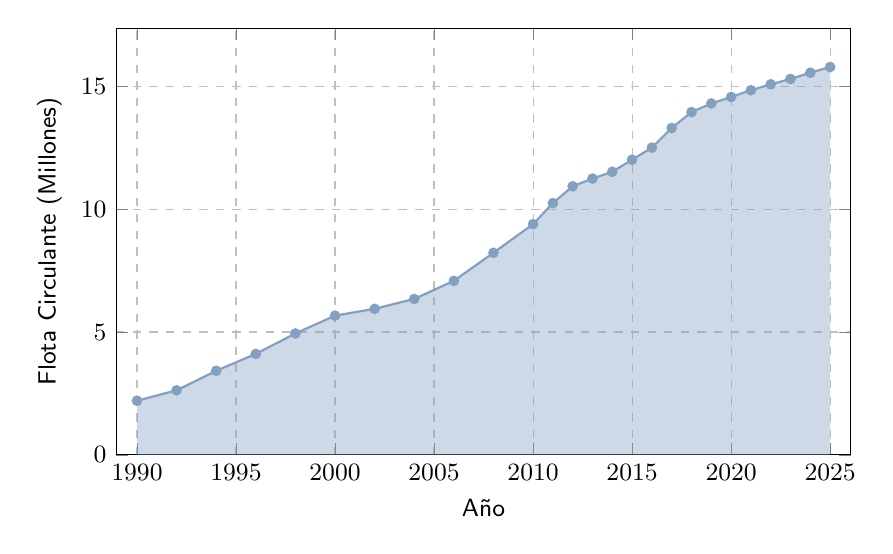
\begin{tikzpicture}[font=\sffamily\small]
    \begin{axis}[
        width=0.9\linewidth,
        height=7cm,
        xlabel={Año},
        ylabel={Flota Circulante (Millones)},
        ymin=0,
        xtick={1990, 1995, 2000, 2005, 2010, 2015, 2020, 2025},
        xticklabel style={/pgf/number format/1000 sep=},
        ymajorgrids=true,
        xmajorgrids=true,
        grid style=dashed,
        enlarge x limits=0.03
    ]
    % Área sombreada bajo la curva
    \addplot[fill=colDatoPrimario, fill opacity=0.4, draw=none] coordinates {
        (1990, 0)
        (1990, 2.203) (1992, 2.627) (1994, 3.420) (1996, 4.109)
        (1998, 4.941) (2000, 5.666) (2002, 5.943) (2004, 6.345)
        (2006, 7.081) (2008, 8.224) (2010, 9.389) (2011, 10.246)
        (2012, 10.930) (2013, 11.245) (2014, 11.520) (2015, 12.012)
        (2016, 12.503) (2017, 13.302) (2018, 13.950) (2019, 14.301)
        (2020, 14.564) (2021, 14.840) (2022, 15.079) (2023, 15.299)
        (2024, 15.552) (2025, 15.784)
        (2025, 0)
    };
    % Línea principal con marcadores
    \addplot[color=colDatoPrimario, thick, mark=*, mark options={fill=colDatoPrimario, draw=colDatoPrimario}, mark size=1.5pt] coordinates {
        (1990, 2.203) (1992, 2.627) (1994, 3.420) (1996, 4.109)
        (1998, 4.941) (2000, 5.666) (2002, 5.943) (2004, 6.345)
        (2006, 7.081) (2008, 8.224) (2010, 9.389) (2011, 10.246)
        (2012, 10.930) (2013, 11.245) (2014, 11.520) (2015, 12.012)
        (2016, 12.503) (2017, 13.302) (2018, 13.950) (2019, 14.301)
        (2020, 14.564) (2021, 14.840) (2022, 15.079) (2023, 15.299)
        (2024, 15.552) (2025, 15.784)
    };
    \end{axis}
    \end{tikzpicture}
    \caption{Evolución de la flota vehicular circulante estimada en Argentina entre 1990 y 2025, expresada en millones de vehículos. La línea y los marcadores representan los valores anuales disponibles; el área sombreada facilita la lectura de su magnitud. Elaboración propia a partir de reportes de \acrshort{acr-afac}.}\label{fig:flota_circulante}
\end{figure}

Como refleja la figura \ref{fig:flota_circulante}, la flota vehicular activa en Argentina experimentó una expansión sostenida entre 1990 y 2025, pasando de aproximadamente 2,2 millones a 15,78 millones de unidades operativas \cite{AFAC2018Flota,AFAC2026Flota}. En los reportes de \acrshort{acr-afac}, la flota circulante comprende automóviles y vehículos comerciales livianos y pesados en condiciones de circular, excluyendo acoplados y remolques; representa una estimación del parque activo bajo esa definición, no el total histórico de unidades patentadas ni la cantidad de viajes realizados. Este incremento acumulado ejerce una presión creciente sobre redes viales consolidadas que poseen una capacidad física fija, agudizando la formación de colas y demoras en las intersecciones urbanas críticas.

Las congestiones vehiculares deterioran las condiciones de operación de la red e incrementan las demoras y las detenciones de los vehículos \cite{calymayor}. En el modelado microscópico, las emisiones de gases como el monóxido de carbono (\acrshort{acr-co}), el dióxido de carbono (\acrshort{acr-co2}), los óxidos de nitrógeno (\acrshort{acr-nox}) y los hidrocarburos no combustionados (\acrshort{acr-hc}) se estiman a partir de variables cinemáticas, entre ellas la velocidad, la aceleración y el tiempo en ralentí \cite{SUMO2026_SUMO}. Este problema es especialmente relevante en ciudades con alta densidad vehicular. En este trabajo se utilizan escenarios sintéticos y un escenario urbano restringido por datos: el microcentro de la Ciudad de Mendoza, delimitado por las avenidas San Martín, Colón, Belgrano y Las Heras.

Frente a la congestión, una alternativa que no requiere modificaciones importantes de la infraestructura consiste en optimizar la gestión del tránsito mediante sistemas de control semafórico adaptativos. Los enfoques tradicionales pueden presentar limitaciones para responder a variaciones en el flujo vehicular \cite{ite_handbook}. En este contexto, los avances en \gls{acr-ia} y en particular el \gls{acr-rl} permiten modelar los semáforos como agentes que aprenden políticas de control a partir de la interacción con el entorno. Las acciones corresponden a cambios de fase y la recompensa puede definirse, por ejemplo, como el negativo del tiempo de espera acumulado. Diversos estudios han mostrado la viabilidad de este enfoque, desde algoritmos tabulares aplicados a una sola intersección \cite{Wiering2000} hasta modelos de redes coordinadas basados en redes neuronales profundas y control multiagente \cite{WeiH2019ASTSCM}.

Sin embargo, la aplicación simultánea de este enfoque en múltiples intersecciones introduce desafíos adicionales. Un esquema centralizado puede resultar poco escalable, pues el espacio de acciones conjunto crece multiplicativamente con el número de intersecciones \cite{marlbook}. En una formulación de \gls{acr-marl} con \gls{acr-il}, cada semáforo optimiza su propia intersección sin considerar explícitamente el efecto de sus decisiones sobre el resto de la red \cite{Ault2022_MARL_Limitations}. Además, como todos los agentes aprenden y modifican sus políticas al mismo tiempo, cada uno observa un entorno no estacionario. Esto dificulta la convergencia de los algoritmos de agente único \cite{foerster2017}.

Por esta razón, este trabajo aborda el problema desde el marco del \gls{acr-marl} cooperativo. Cada controlador aprende a gestionar su propia intersección, pero sus decisiones también buscan evitar que las colas y las demoras se trasladen hacia las intersecciones vecinas. En lugar de asignar una única recompensa idéntica a todos los agentes, el sistema entrega a cada uno una señal que refleja tanto la evolución de la espera local como la de su entorno inmediato. Durante el entrenamiento de las variantes centralizadas, el crítico incorpora además información conjunta de la red. De este modo, cada controlador recibe una señal vinculada con su área de influencia, sin perder de vista el funcionamiento de la red vial en su conjunto.

En este contexto, el objetivo general de este trabajo es desarrollar y evaluar un sistema de control semafórico basado en aprendizaje por refuerzo multiagente para mejorar la operación del tránsito en redes urbanas. En particular, la investigación compara el desempeño de algoritmos de entrenamiento centralizado y ejecución descentralizada (\acrshort{acr-mappo} y \acrshort{acr-happo}) con esquemas de aprendizaje independiente (\acrshort{acr-ippo} e \acrshort{acr-idqn}) bajo condiciones controladas, con el fin de evaluar estrategias de coordinación cooperativa y de tratamiento de la heterogeneidad entre intersecciones. La evaluación empírica se lleva a cabo mediante simulaciones microscópicas en escenarios sintéticos de complejidad creciente y en la red vial modelada del microcentro de la Ciudad de Mendoza, utilizando el control de tiempo fijo como ancla operacional de referencia.

Uno de los aportes metodológicos de este trabajo es representar la espera acumulada por carril mediante una transformación logarítmico-lineal acotada y discretizada en $I$ categorías con resolución no uniforme. Las categorías ofrecen mayor detalle para demoras bajas, agrupan situaciones de espera semejantes y limitan los valores extremos; así, esta representación puede facilitar el tratamiento de variaciones pequeñas y mantener acotado el rango de la observación. El uso de distintas representaciones de estado en el control semafórico con aprendizaje por refuerzo cuenta con antecedentes \cite{genders2018representations}. En esta investigación, la codificación se evalúa como parte del sistema completo; determinar su contribución específica requeriría compararla con otras codificaciones.

Además, se examina si las políticas diferenciadas son adecuadas para intersecciones con geometrías, conjuntos de acciones o demandas distintos, frente a la alternativa de compartir una política. La implementación de \acrshort{acr-happo} adapta la secuencia de actualizaciones de actores, en la que se consideran los cambios previos, con ventajas individuales y señales de recompensa locales-vecinales; en las variantes centralizadas, el crítico es compartido. Esta secuencia distingue su procedimiento de actualización del de \acrshort{acr-mappo}, sin implicar una actualización nueva del crítico ni garantizar superioridad. La comparación con políticas compartidas y con los enfoques locales de \acrshort{acr-ippo} y \acrshort{acr-idqn} permite estudiar esta cuestión en los escenarios considerados.


\section{Motivación}\label{sec:motivacion}

La motivación de este trabajo se centra en estudiar cómo coordinar controladores que aprenden en una misma red vial. El control adaptativo basado en aprendizaje por refuerzo permite ajustar decisiones a las condiciones observadas \cite{MDPI_Infrastructures2025_RLReview}. En una red de múltiples intersecciones, interesa examinar cómo esa adaptación puede incorporar los efectos de las decisiones locales sobre los cruces vecinos.

Las diferencias de demanda, geometría y fases disponibles entre intersecciones motivan, además, el estudio de políticas que puedan adaptarse a esas condiciones. La comparación de \acrshort{acr-mappo} y \acrshort{acr-happo} con los esquemas independientes \acrshort{acr-ippo} e \acrshort{acr-idqn} permite examinar distintas formas de aprendizaje y coordinación bajo una misma formulación del problema.


\section{Organización del Documento}\label{sec:organizacion_documento}

El presente trabajo se estructura de la siguiente manera:

\begin{itemize}
    \item \textbf{Capítulo 1 -- Introducción:} contextualiza la problemática de la congestión vehicular urbana, define los objetivos del proyecto y expone las motivaciones que impulsan esta investigación.
    \item \textbf{Capítulo 2 -- Marco Teórico:} presenta los conceptos fundamentales de la ingeniería de tránsito, la teoría de procesos de decisión de Markov, las redes neuronales profundas y los paradigmas de aprendizaje por refuerzo multiagente.
    \item \textbf{Capítulo 3 -- Metodología:} detalla el diseño metodológico y experimental, la calibración de la demanda vial mediante el estadístico \gls{acr-geh}, el modelado del microcentro de la Ciudad de Mendoza en \gls{acr-sumo} y la formulación algorítmica de los controladores.
    \item \textbf{Capítulo 4 -- Resultados:} presenta la evaluación empírica y comparativa de los algoritmos de control sobre redes sintéticas y el escenario urbano restringido por datos.
    \item \textbf{Capítulo 5 -- Conclusiones:} sintetiza los hallazgos principales, discute las limitaciones del modelo y propone direcciones de investigación futuras.
    \item \textbf{Apéndice A -- Arquitectura de Software:} describe las especificaciones orientadas a objetos, los diagramas de clases \gls{acr-uml} y los patrones de diseño aplicados en el marco computacional \texttt{marlTLC}.
\end{itemize}

\chapter{Marco Teórico}\label{cap:marco_teorico}

\section{Ingeniería de Tránsito y Simulación}\label{sec:ingenieria_transito}

La ingeniería de tránsito se define como aquella fase de la ingeniería de transporte —disciplina que se enmarca tradicionalmente dentro de la ingeniería civil— que se ocupa de la planeación segura y eficiente, el proyecto geométrico y la operación del tránsito por calles y carreteras, sus redes, terminales, tierras adyacentes y su relación con otros modos de transporte \cite{calymayor}. Asimismo, el \textit{Traffic Engineering Handbook} la describe formalmente como la subdisciplina enfocada en la planificación, el diseño geométrico y la operación de redes viales \cite{ite_handbook}. En este trabajo, sus conceptos se abordan desde la perspectiva del modelado computacional y la gestión adaptativa: permiten describir el funcionamiento físico de la red vial, caracterizar la oferta y demanda de circulación, e identificar las variables operacionales sobre las cuales puede intervenir un sistema de control inteligente.

Históricamente, la práctica de la ingeniería de tránsito puso un fuerte énfasis en proveer y ampliar la capacidad física vial mediante la construcción de nuevas obras o el ensanche de calzadas \cite{ite_handbook}. Sin embargo, el crecimiento sostenido del parque automotor evidenció que la ampliación de la infraestructura no constituye una solución definitiva al problema de la congestión. En áreas urbanas consolidadas, además, modificar el trazado vial resulta costoso y geométricamente inviable \cite{calymayor}. Por ello, la práctica contemporánea complementa la infraestructura física con estrategias de control dinámico del tránsito, priorizando la optimización de los recursos existentes mediante dispositivos de control semafórico.

La operación de una red vial puede analizarse a partir de la relación entre la demanda vehicular y la capacidad disponible. La demanda vehicular ($D$) corresponde a la cantidad de vehículos que requieren desplazarse por un determinado sistema vial en un lapso dado, mientras que la oferta vial o capacidad ($c$) representa la cantidad máxima de vehículos que pueden circular por dicho espacio físico bajo determinadas condiciones de operación \cite{calymayor}. Cuando la demanda se aproxima a la capacidad, el tránsito se vuelve inestable; cuando la supera ($D > c$), se presentan condiciones de sobresaturación o flujo forzado, caracterizadas por detenciones frecuentes y grandes demoras. En este sentido, la congestión no se entiende solo como una percepción general de mal funcionamiento, sino como un fenómeno con manifestaciones físicas medibles: demoras, colas y detenciones \cite{fernandez}.

\subsection{Terminología de Tránsito}

Antes de introducir los mecanismos de control y su formulación computacional, conviene precisar algunos términos operativos que se utilizarán de manera recurrente en este documento. Esta aclaración inicial es habitual en manuales de temporización semafórica, donde se advierte que el término fase puede confundirse con movimiento si no se distingue la unidad de control del conjunto de trayectorias servidas \cite{fhwa_signal_timing_manual}, y en estudios de control semafórico basados en aprendizaje por refuerzo, donde los conceptos de movimientos, fases y señales se explicitan antes de formular el problema de decisión \cite{WeiH2019ASTSCM}.

En este contexto, se emplearán las siguientes nociones:

\begin{itemize}
    \item \textbf{Intersección, acceso y carril:} una intersección es el área física y operacional en la que confluyen dos o más corrientes de tránsito. Cada una de las calzadas de aproximación que ingresan a ella constituye un acceso \cite{ite_handbook}, organizándose internamente en uno o más carriles destinados a canalizar los flujos vehiculares \cite{calymayor}.
    \item \textbf{Movimiento vehicular y movimientos en conflicto:} un movimiento vehicular representa la trayectoria específica que describe un vehículo al cruzar la intersección hacia una salida determinada (e.g., giros o movimientos directos) \cite{WeiH2019ASTSCM}. Dos movimientos se consideran en conflicto o incompatibles cuando sus trayectorias se intersectan y generan puntos de conflicto en la intersección (véase la Figura \ref{fig:conflictos_interseccion}), lo que impide su servicio simultáneo por razones de seguridad \cite{fernandez}.
    \item \textbf{Fase, ciclo e intervalo:} una fase representa el estado operativo del semáforo que otorga el derecho de paso a un grupo de movimientos compatibles de manera simultánea \cite{ite_handbook}. La secuencia completa de fases requerida para servir a todos los movimientos de la intersección constituye el ciclo semafórico, mientras que un intervalo es la fracción temporal del ciclo durante la cual las indicaciones del semáforo no varían \cite{calymayor}.
\end{itemize}

La Figura \ref{fig:movimientos_fases_interseccion} muestra una representación típica de estos conceptos para una intersección de cuatro accesos. La convención utilizada por manuales de temporización como el de la FHWA asigna números impares a los giros izquierdos y números pares a los movimientos directos; los giros derechos suelen operar junto con el movimiento directo compatible, mientras que los cruces peatonales se sirven de manera concurrente con la corriente vehicular paralela \cite{fhwa_signal_timing_manual}. Esta representación no fija una geometría particular para el caso de estudio, sino que permite distinguir entre movimiento físico, fase semafórica y usuarios servidos por una misma indicación.

\begin{figure}[H]
    \centering
    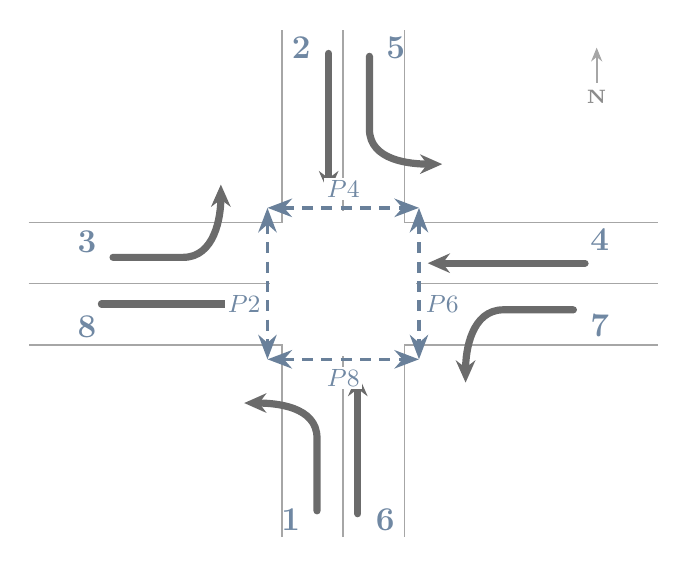
\begin{tikzpicture}[
        x=0.74cm,
        y=0.74cm,
        >=Stealth,
        font=\small,
        veh/.style={-{Stealth[length=8pt,width=7pt]}, line width=2.6pt, black!58, line cap=round},
        ped/.style={<->, dashed, dash pattern=on 4pt off 3pt, line width=1.3pt, colDatoPrimario!80!black},
        num/.style={font=\bfseries\large, colDatoPrimario!85!black},
        pnum/.style={font=\small, colDatoPrimario!85!black},
        road/.style={black!35, line width=0.65pt}
    ]
        % Geometría simplificada siguiendo la disposición de FHWA: calzadas y ejes.
        \draw[road] (-5.4,1.05) -- (-1.05,1.05) -- (-1.05,4.35);
        \draw[road] (1.05,4.35) -- (1.05,1.05) -- (5.4,1.05);
        \draw[road] (5.4,-1.05) -- (1.05,-1.05) -- (1.05,-4.35);
        \draw[road] (-1.05,-4.35) -- (-1.05,-1.05) -- (-5.4,-1.05);
        \draw[road] (-5.4,0) -- (-1.25,0);
        \draw[road] (1.25,0) -- (5.4,0);
        \draw[road] (0,-4.35) -- (0,-1.25);
        \draw[road] (0,1.25) -- (0,4.35);

        % Movimientos vehiculares: números impares para giros izquierdos y pares para directos.
        \draw[veh] (-0.25,3.95) -- (-0.25,1.55);
        \node[num] at (-0.72,4.05) {2};
        \draw[veh] (0.45,3.90) -- (0.45,2.65) to[out=-90,in=180] (1.70,2.05);
        \node[num] at (0.90,4.05) {5};

        \draw[veh] (4.15,0.35) -- (1.45,0.35);
        \node[num] at (4.40,0.75) {4};
        \draw[veh] (3.95,-0.45) -- (2.75,-0.45) to[out=180,in=90] (2.10,-1.70);
        \node[num] at (4.40,-0.72) {7};

        \draw[veh] (0.25,-3.95) -- (0.25,-1.55);
        \node[num] at (0.72,-4.05) {6};
        \draw[veh] (-0.45,-3.90) -- (-0.45,-2.65) to[out=90,in=0] (-1.70,-2.05);
        \node[num] at (-0.90,-4.05) {1};

        \draw[veh] (-4.15,-0.35) -- (-1.45,-0.35);
        \node[num] at (-4.40,-0.75) {8};
        \draw[veh] (-3.95,0.45) -- (-2.75,0.45) to[out=0,in=-90] (-2.10,1.70);
        \node[num] at (-4.40,0.72) {3};

        % Movimientos peatonales concurrentes.
        \draw[ped] (-1.30,1.30) -- (1.30,1.30);
        \draw[ped] (1.30,1.30) -- (1.30,-1.30);
        \draw[ped] (-1.30,-1.30) -- (1.30,-1.30);
        \draw[ped] (-1.30,1.30) -- (-1.30,-1.30);
        \node[pnum, fill=white, inner sep=1pt] at (0,1.62) {$P4$};
        \node[pnum, fill=white, inner sep=1pt] at (1.70,-0.35) {$P6$};
        \node[pnum, fill=white, inner sep=1pt] at (0,-1.62) {$P8$};
        \node[pnum, fill=white, inner sep=1pt] at (-1.70,-0.35) {$P2$};

        \draw[-{Stealth[length=5pt,width=4pt]}, black!35, line width=0.7pt] (4.35,3.45) -- (4.35,4.05);
        \node[font=\scriptsize\bfseries, black!45] at (4.35,3.20) {N};
    \end{tikzpicture}
    \caption{Convención esquemática de movimientos vehiculares, fases y cruces peatonales concurrentes en una intersección de cuatro accesos, adaptada conceptualmente del manual de temporización semafórica de FHWA \cite{fhwa_signal_timing_manual}.}
    \label{fig:movimientos_fases_interseccion}
\end{figure}

\begin{figure}[htp]
    \centering
    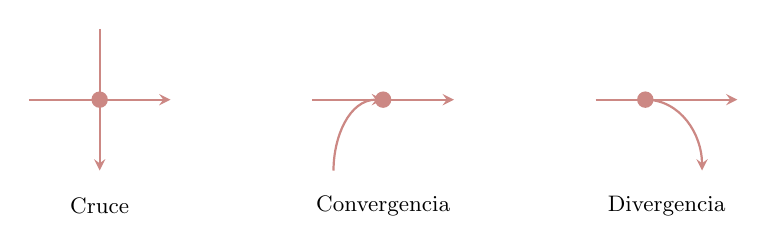
\begin{tikzpicture}[>=stealth, thick, font=\small, scale=0.9, transform shape]
        % Cruce
        \draw[->, colConflicto] (0, 0) -- (2, 0);
        \draw[->, colConflicto] (1, 1) -- (1, -1);
        \filldraw[colConflicto] (1, 0) circle (0.1);
        \node at (1, -1.5) {Cruce};

        % Convergencia
        \draw[->, colConflicto] (4, 0) -- (6, 0);
        \draw[->, colConflicto] (4.3, -1) to[out=90, in=180] (5, 0); 
        \filldraw[colConflicto] (5, 0) circle (0.1);
        \node at (5, -1.5) {Convergencia};

        % Divergencia
        \draw[->, colConflicto] (8, 0) -- (10, 0);
        \draw[->, colConflicto] (8.7, 0) to[out=0, in=90] (9.5, -1);
        \filldraw[colConflicto] (8.7, 0) circle (0.1);
        \node at (9, -1.5) {Divergencia};
    \end{tikzpicture}
    \caption{Representación esquemática de movimientos vehiculares y puntos de conflicto en una intersección semaforizada.}
    \label{fig:conflictos_interseccion}
\end{figure}

En arterias urbanas, el tránsito se desarrolla bajo condiciones de flujo interrumpido: los vehículos no avanzan únicamente por su interacción con otros vehículos, sino también por la presencia de intersecciones, señales y dispositivos de control de tránsito \cite{ite_handbook}. Las intersecciones son puntos críticos de la red porque allí confluyen distintos accesos y movimientos vehiculares de cruce, convergencia y divergencia que pueden resultar incompatibles entre sí. Por ello, su operación requiere ordenar estos movimientos y asignar la prioridad de paso de manera segura y eficiente.

El semáforo es uno de los dispositivos de control de tránsito utilizados para regular la circulación en intersecciones. Su función es asignar la prioridad de paso en forma alternada entre corrientes vehiculares incompatibles, evitando que distintos movimientos intenten ocupar simultáneamente el mismo espacio de cruce \cite{fernandez}. Desde el punto de vista del modelado algorítmico, esta capacidad de modificar la prioridad de paso convierte al semáforo en el actuador mediante el cual un sistema de control puede intervenir sobre la operación de la intersección y afectar, directa o indirectamente, las demoras y colas observadas en la red.

\subsection{Fundamentos de la Dinámica Vehicular}\label{subsec:fundamentos_dinamica_vehicular}

Para modelar y optimizar la operación de una red vial, es necesario caracterizar físicamente el movimiento de los vehículos. La ingeniería de tránsito estudia este fenómeno a partir de las características fundamentales de la corriente de tránsito, que permiten describir las condiciones de operación de una vía o intersección mediante magnitudes observables como el flujo, la velocidad y la densidad \cite{ite_handbook}. Cal y Mayor distingue estas magnitudes entre variables principales, que describen el comportamiento agregado del flujo vehicular, y variables asociadas, que expresan relaciones temporales y espaciales entre vehículos consecutivos \cite{calymayor}.

A nivel macroscópico, la corriente de tránsito se representa mediante variables agregadas como la tasa de flujo, la densidad y los promedios de velocidad. A nivel microscópico, se analizan magnitudes propias de vehículos individuales e interacciones entre pares consecutivos, como la velocidad puntual, el intervalo y el espaciamiento \cite{calymayor}. Esta separación entre escalas es fundamental para el modelado computacional: las variables macroscópicas resumen el estado operacional de los accesos de la red, mientras que las variables microscópicas describen el comportamiento de cada vehículo dentro del simulador \cite{fernandez}. La correspondencia y las relaciones de conversión entre las variables de ambas escalas se resumen en la Tabla \ref{tab:variables_transito}.

En el nivel macroscópico, las variables principales de la corriente de tránsito son:
\begin{itemize}
    \item \textbf{Flujo o tasa de flujo ($q$):} representa la cantidad de vehículos que atraviesan una sección transversal de la vía por unidad de tiempo. Si el período de observación es menor a una hora, se proyecta como una tasa horaria equivalente en vehículos por hora (veh/h), calculada como $q = N/T$, donde $N$ es el número de vehículos observados y $T$ es la duración del intervalo de medición expresado en horas \cite{calymayor}.
    \item \textbf{Densidad o concentración ($k$):} indica el número de vehículos que ocupan simultáneamente una longitud específica de vía, expresada en vehículos por kilómetro (veh/km), calculada como $k = N/d$, donde $d$ representa la longitud del tramo de vía analizado \cite{calymayor}. En la práctica, se suele estimar indirectamente a través del porcentaje de ocupación temporal registrado por detectores inductivos \cite{ite_handbook}.
    \item \textbf{Velocidad media espacial ($v_s$):} es la velocidad media de los vehículos que ocupan un tramo de vía en un instante determinado. Corresponde al promedio armónico de las velocidades puntuales de los vehículos individuales y representa la magnitud de velocidad consistente con la dinámica del flujo espacial \cite{calymayor}.
    \item \textbf{Velocidad media temporal ($v_t$):} representa el promedio aritmético de las velocidades de los vehículos que cruzan una sección transversal fija de la vía durante un período de tiempo determinado \cite{calymayor}.
\end{itemize}

En el nivel microscópico, las variables asociadas describen el movimiento del vehículo individual y la separación entre vehículos consecutivos (véase la Figura \ref{fig:variables_microscopicas}):
\begin{itemize}
    \item \textbf{Velocidad puntual ($v_i$):} es la velocidad instantánea a la que un vehículo individual ($i$) atraviesa una sección transversal específica de la vía.
    \item \textbf{Intervalo temporal ($h$):} es el tiempo transcurrido entre el paso de dos vehículos consecutivos por una sección fija de la calzada, medido respecto a puntos homólogos (e.g., parachoques delanteros) \cite{calymayor}. El intervalo promedio en segundos ($h_{\text{prom}}$) se relaciona con la tasa de flujo como $h_{\text{prom}} = 3600/q$.
    \item \textbf{Espaciamiento simple ($s$):} es la distancia física entre puntos homólogos de dos vehículos consecutivos en un instante de tiempo \cite{calymayor}. El espaciamiento promedio en metros ($s_{\text{prom}}$) se relaciona de forma inversa con la densidad de la corriente de tránsito como $s_{\text{prom}} = 1000/k$.
\end{itemize}

\begin{table}[H]
\centering
\caption{Comparación y correspondencia de variables de tránsito en escalas macroscópica y microscópica.}
\label{tab:variables_transito}
\setlength{\tabcolsep}{4pt}
\begin{tabular}{|p{2.3cm}|p{4.0cm}|p{5.4cm}|}
\hline
\textbf{Escala} & \textbf{Variable Principal} & \textbf{Relación / Conversión} \\ \hline
Macroscópica & Flujo ($q$, veh/h) & $q = 3600 / h_{\text{prom}}$ \\ \cline{2-3}
 & Densidad ($k$, veh/km) & $k = 1000 / s_{\text{prom}}$ \\ \cline{2-3}
 & Velocidad media espacial ($v_s$, km/h) & $q = k \cdot v_s$ \\ \cline{2-3}
 & Velocidad media temporal ($v_t$, km/h) & $v_t = v_s + \frac{\sigma_s^2}{v_s}$ (Relación de Wardrop) \\ \hline
Microscópica & Velocidad puntual ($v_i$, km/h) & Variable individual de cada vehículo \\ \cline{2-3}
 & Intervalo temporal ($h$, s) & Tiempo entre pasos de vehículos sucesivos \\ \cline{2-3}
 & Espaciamiento simple ($s$, m) & Distancia espacial entre parachoques homólogos \\ \hline
\end{tabular}
\end{table}

\begin{figure}[H]
    \centering
    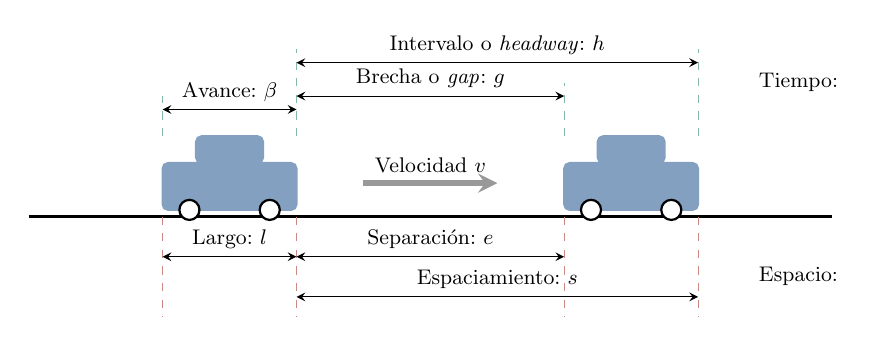
\begin{tikzpicture}[>=stealth, font=\small, scale=0.85, transform shape]
        % Eje de la calle
        \draw[thick] (0,0) -- (12,0);
        
        % Vehículo 1 (Atrás)
        \filldraw[fill=colVehiculo, draw=colVehiculo, thick, rounded corners=2pt] (2, 0.1) rectangle (4, 0.8);
        \filldraw[fill=colVehiculo, draw=colVehiculo, thick, rounded corners=2pt] (2.5, 0.8) rectangle (3.5, 1.2);
        \draw[thick, fill=white] (2.4, 0.1) circle (0.15);
        \draw[thick, fill=white] (3.6, 0.1) circle (0.15);
        
        % Vehículo 2 (Adelante)
        \filldraw[fill=colVehiculo, draw=colVehiculo, thick, rounded corners=2pt] (8, 0.1) rectangle (10, 0.8);
        \filldraw[fill=colVehiculo, draw=colVehiculo, thick, rounded corners=2pt] (8.5, 0.8) rectangle (9.5, 1.2);
        \draw[thick, fill=white] (8.4, 0.1) circle (0.15);
        \draw[thick, fill=white] (9.6, 0.1) circle (0.15);

        % Dirección
        \draw[->, thick, gray!80, line width=2pt] (5, 0.5) -- (7, 0.5) node[midway, above, text=black] {Velocidad $v$};

        % Líneas guía (Espacio)
        \draw[dashed, colSeparacionEsp] (2, 0) -- (2, -1.5); % Trasera V1
        \draw[dashed, colSeparacionEsp] (4, 0) -- (4, -1.5); % Delantera V1
        \draw[dashed, colSeparacionEsp] (8, 0) -- (8, -1.5); % Trasera V2
        \draw[dashed, colSeparacionEsp] (10, 0) -- (10, -1.5); % Delantera V2

        % Líneas guía (Tiempo)
        \draw[dashed, colSeparacionTmp] (4, 1.2) -- (4, 2.5); % Delantera V1 arriba
        \draw[dashed, colSeparacionTmp] (2, 1.2) -- (2, 1.8); % Trasera V1 arriba
        \draw[dashed, colSeparacionTmp] (8, 1.2) -- (8, 2.0); % Trasera V2 arriba
        \draw[dashed, colSeparacionTmp] (10, 1.2) -- (10, 2.5); % Delantera V2 arriba

        % Cotas Espacio (Abajo)
        \draw[<->] (2, -0.6) -- (4, -0.6) node[midway, above] {Largo: $l$};
        \draw[<->] (4, -0.6) -- (8, -0.6) node[midway, above] {Separación: $e$};
        \draw[<->] (4, -1.2) -- (10, -1.2) node[midway, above] {Espaciamiento: $s$};
        \node at (11.5, -0.9) {Espacio:};

        % Cotas Tiempo (Arriba)
        \draw[<->] (2, 1.6) -- (4, 1.6) node[midway, above] {Avance: $\beta$};
        \draw[<->] (4, 1.8) -- (8, 1.8) node[midway, above] {Brecha o \textit{gap}: $g$};
        \draw[<->] (4, 2.3) -- (10, 2.3) node[midway, above] {Intervalo o \textit{headway}: $h$};
        \node at (11.5, 2.0) {Tiempo:};
    \end{tikzpicture}
    \caption{Relaciones temporales y espaciales entre vehículos consecutivos de una corriente de tránsito: intervalo ($h$) y espaciamiento ($s$).}
    \label{fig:variables_microscopicas}
\end{figure}

Estas variables macroscópicas y agregadas se relacionan de manera directa a través de la ecuación fundamental del flujo de tránsito:
\begin{equation}
    q = k \cdot v_s
\end{equation}
donde $q$ es la tasa de flujo, $k$ es la densidad y $v_s$ es la velocidad media espacial. Cabe destacar que la velocidad media espacial ($v_s$) es la única físicamente consistente con esta ecuación fundamental. La velocidad media temporal ($v_t$) difiere de esta debido a que asigna mayor peso a los vehículos más rápidos que cruzan el punto de medición en un lapso dado. La vinculación analítica entre ambas variables se establece formalmente mediante la relación de Wardrop \cite{fernandez}:
\begin{equation}
    v_t = v_s + \frac{\sigma_s^2}{v_s}
\end{equation}
donde $\sigma_s^2$ representa la varianza de la distribución de las velocidades de los vehículos en el espacio. Dado que la varianza es siempre no negativa ($\sigma_s^2 \ge 0$), se cumple que $v_t \ge v_s$, igualándose únicamente en el caso hipotético en que todos los vehículos circulen exactamente a la misma velocidad. En intersecciones semaforizadas, esta relación dinámica permite modelar cómo las interrupciones del semáforo durante la luz roja detienen el flujo ($v_s \to 0$), provocando una acumulación de vehículos que eleva la densidad ($k \to k_{\max}$) y genera colas y demoras asociadas a condiciones de flujo forzado \cite{calymayor}.

\subsubsection{Métricas de Ineficiencia Operativa}

La interrupción del flujo causada por semáforos o saturación genera efectos adversos que los sistemas de control buscan mitigar. Siguiendo la terminología de la ingeniería de tránsito, las principales manifestaciones medibles de esta ineficiencia son las demoras, las colas y las detenciones \cite{fernandez}:
\begin{itemize}
    \item \textbf{Demoras:} Representan el tiempo adicional que un vehículo debe invertir para atravesar una intersección respecto del tiempo que le tomaría circular a velocidad de flujo libre. En intersecciones semaforizadas, una parte de esa demora aparece por la espera normal durante la luz roja. Otras demoras se producen cuando las llegadas de vehículos varían, cuando la demanda se acerca o supera la capacidad de la intersección, o cuando quedan colas sin disiparse al finalizar el verde, de modo que algunos vehículos deben esperar más de un ciclo para cruzar.
    \item \textbf{Colas:} Corresponden al número de vehículos acumulados detrás de una línea de detención a la espera de ser servidos. Esta medida espacial es especialmente relevante porque, cuando la cola supera la longitud del arco de aproximación, puede bloquear la intersección aguas arriba y propagar la congestión al resto de la red.
    \item \textbf{Detenciones:} Cuantifican la cantidad de veces que un vehículo debe reducir su velocidad hasta cero durante el recorrido. Una alta frecuencia de detenciones deteriora la continuidad operativa del flujo y suele asociarse con mayores procesos de aceleración y desaceleración.
\end{itemize}

\subsubsection{Descripción Probabilística del Flujo y Pelotones Vehiculares}

En el modelado de tránsito, las llegadas vehiculares no siempre pueden representarse adecuadamente como una secuencia determinista y constante. Para flujos vehiculares bajos y medios, y cuando las llegadas no están fuertemente condicionadas por semáforos previos, es habitual aproximar el número de vehículos que llega a una sección durante un intervalo de tiempo mediante un proceso de Poisson \cite{calymayor}.

Esta aproximación supone independencia estadística entre llegadas y permite describir la variabilidad observada en la demanda de acceso a una intersección \cite{calymayor}. La probabilidad discreta $P(X)$ de que lleguen exactamente $X$ vehículos en un intervalo de tiempo se define como:
\begin{equation}
    P(X) = \frac{m^X \cdot e^{-m}}{X!}
\end{equation}
donde $X \in \mathbb{N}_0$ es la variable aleatoria discreta que representa el número de arribos vehiculares, $m > 0$ representa el valor esperado o media de llegadas en dicho intervalo, y $e$ es la base del logaritmo natural. Bajo el mismo supuesto, los intervalos de tiempo continuos ($h$) medidos entre vehículos sucesivos se describen mediante una distribución de probabilidad exponencial negativa \cite{calymayor}:
\begin{equation}
    P(h \ge t) = e^{-\frac{q}{3600} \cdot t}
\end{equation}
donde $h$ es el intervalo temporal en segundos, $q$ es el flujo en veh/h, y $t$ es el umbral de tiempo analizado.

Esta representación probabilística asume independencia entre arribos sucesivos, siendo una aproximación válida únicamente para flujos vehiculares bajos o moderados bajo condiciones de flujo libre, donde no exista la influencia de semáforos cercanos aguas arriba \cite{calymayor}. Sin embargo, este supuesto de independencia decae en condiciones de congestión o en redes viales urbanas semaforizadas. En estos casos, la operación de los semáforos interrumpe periódicamente el flujo y agrupa a los vehículos en pelotones (\textit{platoons}), induciendo una fuerte dependencia espacio-temporal y correlación entre arribos consecutivos. La Figura \ref{fig:distribucion_intervalos} presenta una comparación conceptual de la distribución resultante de los intervalos temporales entre vehículos bajo estas dos condiciones operativas.

Esta limitación de los modelos analíticos tradicionales (como los de Poisson o teoría de colas clásica) justifica la necesidad de recurrir a la simulación microscópica de tránsito. En un simulador como SUMO, la formación, dispersión e interacción de pelotones vehiculares emergen de manera natural a partir de los modelos de seguimiento de vehículos y cambio de carril, permitiendo evaluar el control semafórico bajo flujos dinámicos realistas. Asimismo, incorporar arribos estocásticos no Poissonianos, perfiles de demanda variables y la inicialización de múltiples corridas con diferentes semillas aleatorias en el simulador es un procedimiento estándar para evaluar la robustez y capacidad de adaptación de cualquier esquema de control dinámico ante la incertidumbre operativa \cite{calymayor}; esto permite asegurar que los algoritmos sean capaces de responder ante fluctuaciones dinámicas del tráfico en tiempo real, en lugar de optimizarse para una secuencia de flujo determinista y artificial \cite{ite_handbook}.

\begin{figure}[H]
\centering
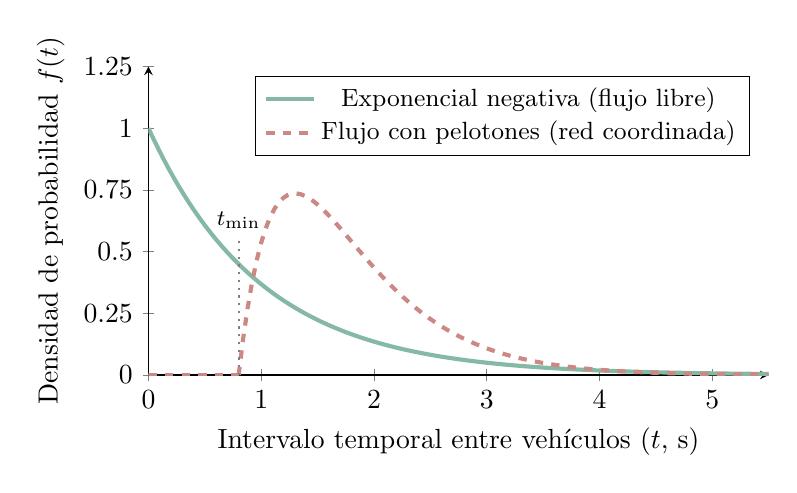
\begin{tikzpicture}
\begin{axis}[
  width=0.78\textwidth,
  height=5.5cm,
  xlabel={Intervalo temporal entre veh\'{i}culos ($t$, s)},
  ylabel={Densidad de probabilidad $f(t)$},
  xmin=0, xmax=5.5,
  ymin=0, ymax=1.25,
  xtick={0,1,2,3,4,5},
  ytick={0,0.25,0.50,0.75,1.00,1.25},
  legend style={at={(0.97,0.97)}, anchor=north east, font=\small},
  axis lines=left,
  every axis plot/.append style={line width=1.5pt}
]
  %% Curva 1: Exponencial negativa (flujo libre / Poisson)
  \addplot[color=colFlujoLibre, domain=0:5.5, samples=120]
    {exp(-x)};
  \addlegendentry{Exponencial negativa (flujo libre)}

  %% Curva 2: Gamma desplazada (flujo con pelotones)
  \addplot[color=colConflicto, dashed, domain=0:0.799, samples=5]
    {0};
  \addplot[color=colConflicto, dashed, domain=0.8:5.5, samples=120]
    {4*(x-0.8)*exp(-2*(x-0.8))};
  \addlegendentry{Flujo con pelotones (red coordinada)}

  %% Linea vertical en t_min
  \draw[dotted, thick, gray] (axis cs:0.8,0) -- (axis cs:0.8,0.55)
    node[above, font=\footnotesize, black] {$t_{\min}$};
\end{axis}
\end{tikzpicture}
\caption{Comparación esquemática de la distribución de intervalos temporales entre vehículos en flujo libre (exponencial negativa, consistente con el proceso de Poisson) y en flujo coordinado por semáforos (distribución desplazada con zona de exclusión física $t_{\min}$ y pico característico de pelotón).}
\label{fig:distribucion_intervalos}
\end{figure}

\subsection{Sistemas de Control de Tránsito}

Para mitigar los conflictos de tránsito e incrementar la seguridad en las intersecciones urbanas de flujo interrumpido, se emplean sistemas de control de tránsito \cite{ite_handbook}. El dispositivo de control por excelencia en estos nodos es el semáforo, definido como un dispositivo electrónico que regula la circulación de vehículos asignando el derecho de paso alternado mediante indicaciones luminosas rojas, amarillas y verdes \cite{calymayor}.

En el modelado algorítmico, los semáforos y sus parámetros de configuración constituyen los elementos actuadores de la red. La modificación de la duración del verde efectivo, la secuencia de fases y la sincronización entre nodos define el conjunto de intervenciones dinámicas mediante las cuales el sistema de control busca optimizar el paso vehicular.

Sobre esta base terminológica, la programación temporal de un semáforo se describe mediante la duración de las fases, la longitud de ciclo y la definición de los intervalos de transición y despeje. Estos parámetros determinan cuánto tiempo recibe prioridad cada conjunto de movimientos compatibles y condicionan directamente la capacidad de descarga, las demoras y la seguridad operacional de la intersección \cite{ite_handbook}.

En relación con los giros izquierdos, los manuales de temporización distinguen entre operación permisiva, protegida y protegida-permisiva. En una fase permisiva, el giro se ejecuta aprovechando brechas en la corriente opuesta; en una fase protegida, el giro recibe una indicación exclusiva y los movimientos conflictivos permanecen detenidos; en una fase protegida-permisiva, ambas condiciones se combinan durante distintos intervalos del ciclo \cite{fhwa_signal_timing_manual}. Para el presente trabajo, la distinción resulta útil porque muestra que una fase no es solo un color del semáforo, sino una regla operacional que habilita ciertos movimientos, impone cesión de paso en otros y restringe los movimientos en conflicto.

Para garantizar la seguridad vial, las transiciones entre fases no pueden ejecutarse de manera instantánea, sino que deben respetar intervalos de cambio y despeje ($t_{\text{amarillo}} + t_{\text{rojo\_todo}}$) \cite{ite_handbook}. En esta investigación, esos tiempos se consideran restricciones operativas de seguridad previamente definidas en la configuración del simulador y del sistema semafórico. En consecuencia, su determinación no forma parte del proceso de decisión del agente, cuyo control se limita a la selección o extensión de fases dentro de un esquema temporal compatible con dichas restricciones.

\subsubsection{Modelado de la Capacidad y el Verde Efectivo}

Desde el punto de vista operativo, la capacidad de descarga de un acceso semaforizado depende del tiempo efectivo de servicio que recibe cada fase y de la tasa con la que la fila puede disiparse cuando el movimiento tiene prioridad \cite{fernandez}. En la práctica, la descarga observada no depende solo de la duración nominal del verde, sino también de pérdidas de arranque, transiciones y otras restricciones temporales del control, como se ilustra conceptualmente en la Figura \ref{fig:verde_efectivo}. En este trabajo, estos efectos no se modelan mediante fórmulas analíticas de capacidad, sino mediante la dinámica microscópica del simulador y la configuración temporal del sistema semafórico, ya que esas interacciones determinan las colas, demoras y detenciones que el controlador busca mejorar.

\begin{figure}[H]
    \centering
    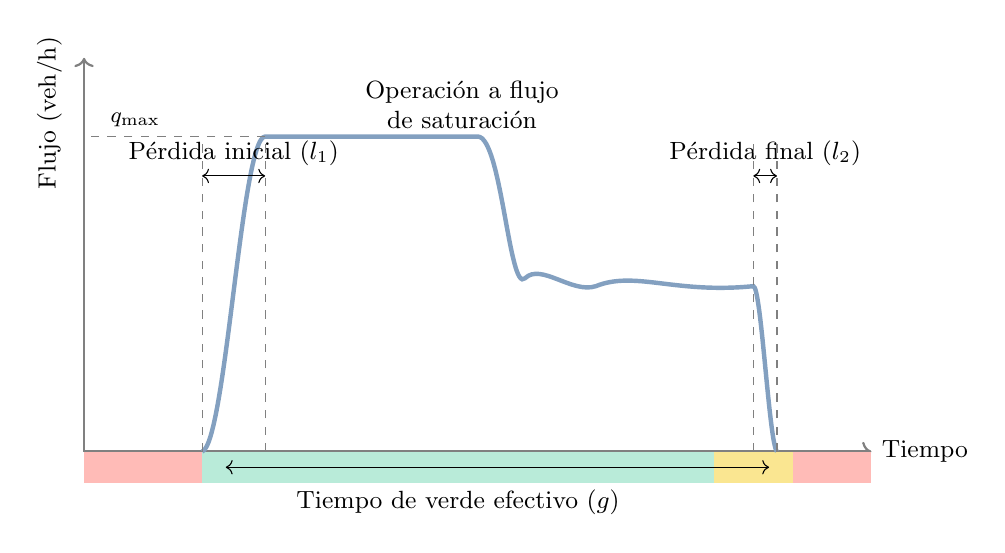
\begin{tikzpicture}[font=\small]
    % Ejes
    \draw[->, thick, gray] (0,0) -- (10,0) node[right, text=black] {Tiempo};
    \draw[->, thick, gray] (0,0) -- (0,5) node[above, text=black, rotate=90, anchor=south, yshift=1ex, xshift=-2em] {Flujo (veh/h)};

    % Fases semáforo (barra inferior)
    \filldraw[fill=colSemaforoRojo, draw=none] (0,-0.4) rectangle (1.5,0); % Rojo
    \filldraw[fill=colSemaforoVerde, draw=none] (1.5,-0.4) rectangle (8,0); % Verde
    \filldraw[fill=colSemaforoAmarillo, draw=none] (8,-0.4) rectangle (9,0); % Amarillo
    \filldraw[fill=colSemaforoRojo, draw=none] (9,-0.4) rectangle (10,0); % Rojo

    \node at (4.75, -0.65) {Tiempo de verde efectivo ($g$)};
    \draw[<->] (1.8, -0.2) -- (8.7, -0.2);

    % Curva de flujo
    \draw[color=colDatoPrimario, ultra thick] 
        (1.5, 0) .. controls (1.8, 0.1) and (2.0, 4.0) .. (2.3, 4.0) -- 
        (5.0, 4.0) .. controls (5.3, 4.0) and (5.4, 2.0) .. (5.6, 2.2) .. controls (5.8, 2.4) and (6.2, 2.0) .. (6.5, 2.1) .. controls (7.0, 2.3) and (7.5, 2.0) .. (8.5, 2.1) .. controls (8.6, 2.1) and (8.7, 0.1) .. (8.8, 0);

    % Etiquetas
    \draw[dashed, gray] (2.3, 4.0) -- (0, 4.0);
    \node[above, font=\footnotesize] at (0.65, 4.0) {$q_{\max}$};
    \node[align=center] at (4.8, 4.4) {Operación a flujo\\ de saturación};
    
    \draw[<->] (1.5, 3.5) -- (2.3, 3.5) node[midway, above] {Pérdida inicial ($l_1$)};
    \draw[dashed, gray] (1.5, 0) -- (1.5, 4);
    \draw[dashed, gray] (2.3, 0) -- (2.3, 4);

    \draw[<->] (8.5, 3.5) -- (8.8, 3.5) node[midway, above] {Pérdida final ($l_2$)};
    \draw[dashed, gray] (8.5, 0) -- (8.5, 4);
    \draw[dashed, gray] (8.8, 0) -- (8.8, 4);
    \end{tikzpicture}
    \caption{Distribución temporal de la tasa de descarga y pérdidas asociadas durante un intervalo de verde en una aproximación semaforizada.}
    \label{fig:verde_efectivo}
\end{figure}

\subsubsection{Clasificación de los Controladores de Semáforos}

De acuerdo con su mecanismo operativo y su grado de respuesta a la demanda vehicular, los controladores de semáforos se clasifican clásicamente en control de tiempo fijo y control accionado por el tránsito \cite{ite_handbook}. En el primero, los planes de señales se repiten de manera preprogramada a partir de datos históricos y no cambian en respuesta a la demanda instantánea. En el segundo, la intersección utiliza detectores en los accesos para variar dinámicamente el inicio o la duración de las fases según la demanda observada en tiempo real.

Incluso en los esquemas accionados, la operación permanece sujeta a parámetros límite de seguridad y funcionamiento, como el verde mínimo ($g_{\min}$) y el verde máximo ($g_{\max}$) \cite{ite_handbook}. Estos parámetros restringen cuánto puede sostenerse o finalizarse una fase y, en este trabajo, forman parte de las condiciones operativas dentro de las cuales el controlador toma decisiones.

\subsection{Simulación de Tránsito}

Debido a la densidad y complejidad de la red urbana moderna, la sincronización y optimización de los tiempos de semáforos no pueden resolverse adecuadamente con modelos estáticos bajo condiciones dinámicas, por lo que se recurre a aproximaciones computacionales basadas en simulación de tránsito \cite{ite_handbook}. De acuerdo con la taxonomía clásica \cite{fernandez}, estos modelos pueden organizarse en tres niveles de resolución. Los modelos macroscópicos describen el tránsito de manera agregada mediante variables como flujo, densidad y velocidad; los modelos mesoscópicos representan entidades intermedias, como grupos o pelotones de vehículos. Ambos niveles son útiles para estudiar fenómenos de red, pero no ofrecen el detalle necesario para observar cómo las decisiones semafóricas afectan, paso a paso, la formación de colas y la interacción local entre vehículos en una intersección.

Para el presente trabajo, el nivel de mayor interés es el microscópico, ya que representa explícitamente a cada vehículo, su ruta y su movimiento dentro de la red \cite{fernandez}. SUMO (\textit{Simulation of Urban MObility}) se ubica en esta categoría: es un simulador de tránsito microscópico, multimodal y de código abierto, diseñado para representar demandas vehiculares sobre redes viales y evaluar problemas de gestión del tránsito \cite{SUMO2018_SUMO,sumo-doc}. En SUMO, la evolución vehicular es continua en el espacio y discreta en el tiempo; además, el entorno permite modelar calles con múltiples carriles, cambios de carril, distintos tipos de vehículos, rutas individuales, semáforos y salidas de simulación a nivel de vehículo, carril, arco o detector \cite{sumo-doc}.
Esta granularidad vuelve a la simulación microscópica especialmente adecuada para estudiar control semafórico mediante aprendizaje por refuerzo. Las decisiones sobre fases y tiempos de servicio no se evalúan mediante una fórmula cerrada de demora, sino observando sus consecuencias sobre la dinámica simulada: colas, tiempos de espera, detenciones, ocupación de carriles y propagación de congestión. Por ello, la simulación microscópica constituye el puente natural entre el problema de tránsito y su formulación computacional, al permitir que el controlador interactúe con un entorno dinámico y medible durante la ejecución.

\subsubsection{Modelos Microscópicos de Comportamiento Vehicular}

En este contexto, el simulador de tránsito constituye el entorno operativo sobre el cual se formaliza el problema de control semafórico. En SUMO, una intersección semaforizada se estructura mediante tres componentes geométricos y lógicos principales bajo el sentido de circulación por la derecha (véase la Figura \ref{fig:sumo_intersection_elements}) \cite{sumo-doc}:
\begin{itemize}
    \item \textbf{Carriles entrantes ($L_{\text{in}}$) y salientes ($L_{\text{out}}$):} Los carriles entrantes conducen el flujo vehicular hacia la línea de detención de la intersección por la derecha de cada acceso, mientras que los carriles salientes reciben el flujo descargado tras cruzar el nodo.
    \item \textbf{Líneas de detención (\textit{stop lines}):} Delimitación física continua en color blanco en el límite de los carriles entrantes $L_{\text{in}}$ con el área interna de cruzamiento (\textit{junction}).
    \item \textbf{Enlaces de conexión (*links*):} Rutas internas que conectan un carril entrante especifico con un carril saliente de destino. A cada enlace se le asigna un estado semafórico instantáneo ($G$ para verde prioritario, $g$ para verde permisivo, y $r$ para rojo o detención). Como se ilustra en la Figura \ref{fig:sumo_intersection_elements}, mientras los movimientos directos se encuentran habilitados en verde ($G$), el giro a la izquierda en conflicto (representado por el enlace en rojo salmón) se mantiene retenido en luz roja ($r$) para prevenir colisiones.
\end{itemize}
Esta representación es compatible con la formulación algorítmica del problema, donde una acción consiste en seleccionar una fase que habilita un conjunto de enlaces compatibles mientras mantiene en rojo ($r$) los movimientos en conflicto.

\begin{figure}[H]
    \centering
    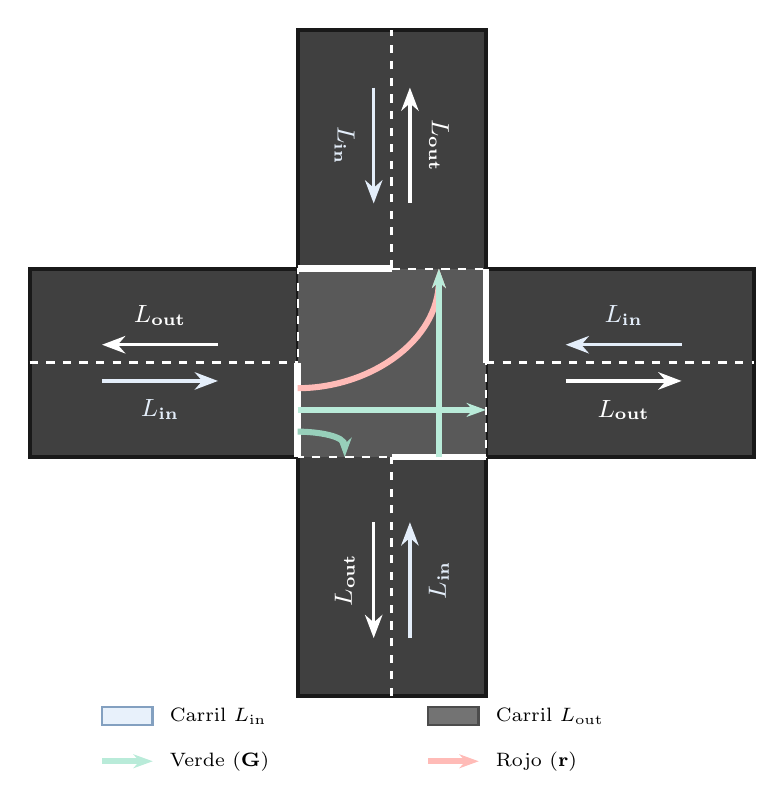
\begin{tikzpicture}[
        scale=0.92,
        font=\small,
        >=Stealth,
        % Estilos de Diseñador Gráfico Experto (Escala de Grises/Asfalto + Alto Contraste)
        roadAsphalt/.style={fill=black!75, draw=black!90, line width=1.4pt},
        laneInBg/.style={fill=colEntorno!25, draw=colEntorno!80!black, line width=1pt},
        laneOutBg/.style={fill=black!55, draw=black!40, line width=1pt},
        stopLine/.style={draw=white, line width=2.5pt},
        dashDivider/.style={draw=white, dashed, line width=1pt},
        % Conexiones de tráfico (Links) en tonos vibrantes
        linkStraight/.style={-{Stealth[length=7pt,width=5pt]}, line width=2.2pt, colSemaforoVerde},
        linkLeft/.style={-{Stealth[length=7pt,width=5pt]}, line width=2.2pt, colSemaforoRojo},
        linkRight/.style={-{Stealth[length=7pt,width=5pt]}, line width=2.2pt, colInterfaz!90!black}
    ]

        % 1. BASE DE CALZADA DE ASFALTO (Tránsito por la Derecha - RHT Argentina)
        \fill[roadAsphalt] (-5.0, -1.3) rectangle (5.0, 1.3);
        \fill[roadAsphalt] (-1.3, -4.6) rectangle (1.3, 4.6);

        % Área interna de cruzamiento (Junction Box)
        \fill[black!65] (-1.3, -1.3) rectangle (1.3, 1.3);
        \draw[white!40, dashed, line width=0.8pt] (-1.3, -1.3) rectangle (1.3, 1.3);

        % Líneas divisorias de carril (Líneas blancas discontinuas)
        \draw[dashDivider] (-5.0, 0) -- (-1.3, 0);
        \draw[dashDivider] (1.3, 0) -- (5.0, 0);
        \draw[dashDivider] (0, 1.3) -- (0, 4.6);
        \draw[dashDivider] (0, -4.6) -- (0, -1.3);

        % 2. LÍNEAS DE DETENCIÓN (Stop Lines en los carriles entrantes L_in)
        \draw[stopLine] (-1.3, -1.3) -- (-1.3, 0);   % Oeste L_in (carril inferior)
        \draw[stopLine] (1.3, 0) -- (1.3, 1.3);      % Este L_in (carril superior)
        \draw[stopLine] (-1.3, 1.3) -- (0, 1.3);     % Norte L_in (carril izquierdo)
        \draw[stopLine] (0, -1.3) -- (1.3, -1.3);    % Sur L_in (carril derecho)

        % 3. ETIQUETAS DE CARRILES Y SENTIDOS DE CIRCULACIÓN (Manejo por la Derecha / Argentina)
        % Acceso Oeste (y < 0 es L_in ingresando al Este; y > 0 es L_out saliendo al Oeste)
        \node[font=\small\bfseries, colEntorno!30] at (-3.2, -0.65) {$L_{\text{in}}$};
        \draw[->, colEntorno!30, line width=1.2pt] (-4.0, -0.25) -- (-2.4, -0.25);
        \node[font=\small\bfseries, white!85] at (-3.2, 0.65) {$L_{\text{out}}$};
        \draw[<-, white!80, line width=1.2pt] (-4.0, 0.25) -- (-2.4, 0.25);

        % Acceso Este (y > 0 es L_in ingresando al Oeste; y < 0 es L_out saliendo al Este)
        \node[font=\small\bfseries, colEntorno!30] at (3.2, 0.65) {$L_{\text{in}}$};
        \draw[<-, colEntorno!30, line width=1.2pt] (2.4, 0.25) -- (4.0, 0.25);
        \node[font=\small\bfseries, white!85] at (3.2, -0.65) {$L_{\text{out}}$};
        \draw[->, white!80, line width=1.2pt] (2.4, -0.25) -- (4.0, -0.25);

        % Acceso Norte (x < 0 es L_in ingresando al Sur; x > 0 es L_out saliendo al Norte)
        \node[font=\small\bfseries, colEntorno!30, rotate=-90] at (-0.65, 3.0) {$L_{\text{in}}$};
        \draw[->, colEntorno!30, line width=1.2pt] (-0.25, 3.8) -- (-0.25, 2.2);
        \node[font=\small\bfseries, white!85, rotate=-90] at (0.65, 3.0) {$L_{\text{out}}$};
        \draw[<-, white!80, line width=1.2pt] (0.25, 3.8) -- (0.25, 2.2);

        % Acceso Sur (x > 0 es L_in ingresando al Norte; x < 0 es L_out saliendo al Sur)
        \node[font=\small\bfseries, colEntorno!30, rotate=90] at (0.65, -3.0) {$L_{\text{in}}$};
        \draw[->, colEntorno!30, line width=1.2pt] (0.25, -3.8) -- (0.25, -2.2);
        \node[font=\small\bfseries, white!85, rotate=90] at (-0.65, -3.0) {$L_{\text{out}}$};
        \draw[<-, white!80, line width=1.2pt] (-0.25, -3.8) -- (-0.25, -2.2);

        % 4. ENLACES INTERNOS DE CRUZAMIENTO (SUMO Links para RHT)
        % Movimientos desde Oeste L_in (y = -0.65):
        \draw[linkStraight] (-1.3, -0.65) -- (1.3, -0.65); % Directo a Este (Verde G)
        \draw[linkLeft] (-1.3, -0.35) to[out=0, in=-90] (0.65, 1.3); % Giro Izquierda a Norte (Rojo r / Salmón)
        \draw[linkRight] (-1.3, -0.95) to[out=0, in=90] (-0.65, -1.3); % Giro Derecha a Sur (Verde Menta g)

        % Movimiento desde Sur L_in (x = 0.65):
        \draw[linkStraight] (0.65, -1.3) -- (0.65, 1.3); % Directo Sur a Norte (Verde G)

        % 5. LEYENDA ESPACIADA AL PIE (Textos ultra-cortos sin superposición)
        \begin{scope}[shift={(0, -5.4)}]
            % Fila 1: Carriles
            \draw[draw=colEntorno!80!black, fill=colEntorno!25, line width=1pt] (-4.0, 0.4) rectangle (-3.3, 0.65);
            \node[anchor=west, font=\scriptsize] at (-3.2, 0.52) {Carril $L_{\text{in}}$};

            \draw[draw=black!70, fill=black!55, line width=1pt] (0.5, 0.4) rectangle (1.2, 0.65);
            \node[anchor=west, font=\scriptsize] at (1.3, 0.52) {Carril $L_{\text{out}}$};

            % Fila 2: Enlaces semafóricos
            \draw[linkStraight] (-4.0, -0.1) -- (-3.3, -0.1);
            \node[anchor=west, font=\scriptsize] at (-3.2, -0.1) {Verde (\textbf{G})};

            \draw[linkLeft] (0.5, -0.1) -- (1.2, -0.1);
            \node[anchor=west, font=\scriptsize] at (1.3, -0.1) {Rojo (\textbf{r})};
        \end{scope}
    \end{tikzpicture}
    \caption{Elementos geométricos y conexiones de una intersección semaforizada en SUMO bajo sentido de circulación por la derecha (Argentina): carriles entrantes ($L_{\text{in}}$), salientes ($L_{\text{out}}$), líneas de detención y enlaces de cruzamiento (\textit{links}) en verde prioritario (\textbf{G}) y rojo retenido en conflicto (\textbf{r}).}
    \label{fig:sumo_intersection_elements}
\end{figure}

\subsubsection{Componentes y Configuración de SUMO}

Para la generación, edición y control en tiempo real de los escenarios de simulación microscópica, el entorno SUMO se complementa con un conjunto integrado de herramientas y librerías auxiliares \cite{SUMO2018_SUMO, sumo_doc_2025}:
\begin{itemize}
    \item \textbf{\textit{netedit}:} Herramienta gráfica que permite proyectar y editar la geometría y la lógica operacional de la red vial de forma interactiva. Facilita la creación y modificación bidireccional de nodos, accesos, carriles, restricciones de giro, conexiones internas (\textit{links}), sensores inductivos y programas de temporización semafórica.
    \item \textbf{\textit{osmwebwizard}:} Herramienta automatizada con interfaz web que permite importar áreas geográficas reales desde OpenStreetMap (OSM) y transformarlas al formato nativo de SUMO, extrayendo la topología urbana, los límites de velocidad y perfiles sintéticos de demanda vehicular.
    \item \textbf{\textit{TraCI} (\textit{Traffic Control Interface}):} Protocolo de comunicación cliente-servidor mediante sockets TCP que habilita la interacción dinámica a paso discreto entre la simulación y scripts externos de control \cite{sumo-doc}. A través de TraCI, los agentes de aprendizaje por refuerzo recolectan observaciones del estado del tránsito (colas, velocidades, ocupación) e imponen decisiones sobre las fases del semáforo.
\end{itemize}

Desde la perspectiva del modelado computacional, la ejecución de una simulación microscópica en SUMO requiere una especificación mínima de archivos de configuración en formato XML \cite{sumo_doc_2025}, cuyos componentes principales se resumen en la Tabla \ref{tab:sumo_input_files}:
\begin{itemize}
    \item \textbf{Archivo de red (\texttt{.net.xml}):} Define la estructura física e infraestructura de la red vial, incluyendo las coordenadas nodales, la geometría de arcos, los carriles por acceso, las conexiones de cruzamiento y la lógica de accionamiento semafórico.
    \item \textbf{Archivo de rutas (\texttt{.rou.xml}):} Especifica las características de la flota vehicular (dimensiones, aceleración, velocidad deseada y modelo de seguimiento) junto con los itinerarios o flujos de origen a destino.
    \item \textbf{Archivo TAZ (\texttt{.taz.xml}, \textit{Traffic Analysis Zones}):} Delimita las zonas de análisis de tráfico para asignar espacialmente las matrices de origen y destino de los desplazamientos.
    \item \textbf{Archivo de elementos adicionales (\texttt{.add.xml}):} Incorpora dispositivos de medición (como detectores de bucle inductivo E1 y E2), paradas de transporte público o programas semafóricos personalizados.
    \item \textbf{Archivo maestro de configuración (\texttt{.sumocfg}):} Integra las referencias a los archivos de red, rutas y adicionales, y fija los parámetros del horizonte temporal de simulación (duración del paso $\Delta t$, tiempos de inicio y fin, e indicadores de salida).
\end{itemize}

\begin{table}[H]
\centering
\caption{Requerimientos mínimos de archivos de configuración para la simulación en SUMO \cite{sumo_doc_2025}.}
\label{tab:sumo_input_files}
\setlength{\tabcolsep}{4pt}
\small
\begin{tabular}{|p{3.0cm}|p{2.5cm}|p{8.5cm}|}
\hline
\textbf{Archivo XML} & \textbf{Extensión} & \textbf{Función en el Modelo Computacional} \\ \hline
Red Vial & \texttt{.net.xml} & Topología física, accesos, carriles, enlaces y semáforos. \\ \hline
Rutas y Demanda & \texttt{.rou.xml} & Tipos de vehículos, modelos de seguimiento e itinerarios. \\ \hline
Zonas TAZ & \texttt{.taz.xml} & Zonas de origen y destino para matrices de demanda. \\ \hline
Elementos Adicionales & \texttt{.add.xml} & Sensores inductivos E1/E2, telemetría y programas auxiliares. \\ \hline
Configuración Maestra & \texttt{.sumocfg} & Unificación de archivos, resolución temporal ($\Delta t$) y registros. \\ \hline
\end{tabular}
\end{table}

\subsubsection{Métricas de Evaluación Operacional y Aprendizaje}

Para evaluar rigurosamente el impacto de las estrategias de control semafórico tanto desde la perspectiva de la ingeniería de tránsito como del aprendizaje automático, este trabajo distingue cuatro métricas fundamentales de evaluación:

\begin{itemize}
    \item \textbf{Emisión de Gases $\text{CO}_2$:} Cuantifica el impacto ambiental y la ineficiencia energética del flujo vehicular. En SUMO, las emisiones se estiman mediante modelos de emisión microscópicos (como HBEFA o PHEMlight \cite{sumo-doc}), relacionando instantáneamente la masa de $\text{CO}_2$ emitida en gramos con los perfiles de velocidad, aceleración y tiempo en ralentí (\textit{idling}) de cada vehículo. Una reducción en la masa total de $\text{CO}_2$ refleja mayor fluidez y menor frecuencia de detenciones.
    \item \textbf{Tiempo de Espera Promedio Global y por Agente:} Métrica operacional primaria en ingeniería de tránsito \cite{calymayor}. El tiempo de espera cuantifica la acumulación en segundos que un vehículo permanece detenido (velocidad $v < 0.1$ m/s) antes de cruzar la intersección. Se evalúa a nivel local por cada agente $i$ (intersección) y de forma agregada a nivel global de la red vial, permitiendo medir la reducción directa de la demora operacional.
    \item \textbf{Recompensa Acumulada Descontada:} Métrica interna de RL/MARL definida como el retorno episódico $G_0 = \sum_{t=0}^T \gamma^t R_t$. Expresa la capacidad del agente para maximizar de forma persistente su objetivo escalar proyectado en el tiempo \cite{suttonRL}.
    \item \textbf{Valores de Pérdida (\textit{Loss Values}):} Indicadores de diagnóstico durante el entrenamiento en DRL/MADRL \cite{yu2022surprising}. Incluyen la pérdida de política o actor ($\mathcal{L}^{\text{CLIP}}$), la pérdida de error cuadrático medio de la función de valor del crítico ($\mathcal{L}^{\text{VF}}$) y el término de entropía de la política ($S[\pi]$). Su seguimiento permite detectar inestabilidades del gradiente, monitorear la tasa de convergencia y prevenir el colapso prematuro de la política (\textit{policy collapse}).
\end{itemize}


\section{Aprendizaje por Refuerzo (RL)}

Dentro del aprendizaje automático suelen distinguirse tres paradigmas principales. En el aprendizaje supervisado, el modelo se entrena a partir de ejemplos etiquetados que indican la salida esperada para cada entrada. En el aprendizaje no supervisado, en cambio, se busca descubrir estructura en datos no etiquetados, por ejemplo mediante agrupamiento o reducción de dimensionalidad. El aprendizaje por refuerzo (\textit{Reinforcement Learning}, RL) aborda un problema distinto: una entidad que toma decisiones debe aprender, mediante interacción con un entorno, qué acciones elegir para maximizar una señal de recompensa acumulada a largo plazo \cite{suttonRL}.

Esta diferencia es central. En RL no existe, en general, un supervisor que indique cuál era la acción correcta en cada situación. El agente aprende por experiencia, ensayando acciones, observando sus consecuencias y ajustando su comportamiento a partir de las recompensas obtenidas. Además, las consecuencias relevantes de una acción no siempre se manifiestan de forma inmediata: una decisión puede producir una recompensa baja en el corto plazo, pero conducir a estados favorables en el futuro. Por este motivo, el aprendizaje por refuerzo se ocupa explícitamente del problema de la recompensa diferida y de la asignación de crédito a decisiones pasadas \cite{suttonRL}.

La formulación básica distingue entre el \textit{agente} (\textit{agent}), que aprende y toma decisiones, y el \textit{entorno} (\textit{environment}), que representa todo aquello externo al agente con lo cual este interactúa. En cada paso temporal, el agente observa una situación del entorno, selecciona una acción y recibe como respuesta una nueva situación junto con una recompensa. El comportamiento del agente está determinado por una \textit{política} (\textit{policy}), denotada por $\pi$, que especifica cómo se eligen las acciones a partir de los estados u observaciones disponibles. La \textit{señal de recompensa} (\textit{reward signal}) define el objetivo inmediato del problema, mientras que la \textit{función de valor} estima la conveniencia de estados o acciones en términos de recompensa futura esperada. Sutton y Barto también distinguen el \textit{modelo} del entorno, entendido como una descripción que permite predecir sus transiciones y recompensas; cuando dicho modelo no se conoce o no se utiliza explícitamente, se habla de métodos libres de modelo (\textit{model-free}).

Un aspecto característico de RL es el dilema entre exploración y explotación. El agente debe explotar acciones que, según su experiencia, producen buenos resultados, pero también debe explorar alternativas menos conocidas que podrían conducir a políticas superiores. Si explora demasiado, desperdicia oportunidades de obtener recompensa; si explota demasiado pronto, puede converger a comportamientos subóptimos. Este equilibrio es especialmente relevante en problemas de control, donde las acciones modifican la experiencia futura disponible para el aprendizaje \cite{suttonRL}.

\subsection{El Proceso de Decisión de Markov (MDP)}

El marco matemático estándar para estudiar problemas de aprendizaje por refuerzo de un solo agente es el Proceso de Decisión de Markov (\textit{Markov Decision Process}, MDP). En un MDP finito, el agente y el entorno interactúan en una secuencia de pasos temporales discretos $t = 0, 1, 2, \dots$. En cada instante $t$, el agente recibe una representación del estado del entorno $S_t \in \mathcal{S}$ y selecciona una acción $A_t \in \mathcal{A}(S_t)$. Como consecuencia de esa acción, el entorno emite una recompensa numérica $R_{t+1} \in \mathcal{R}$ y transita a un nuevo estado $S_{t+1}$ \cite{suttonRL}. Este ciclo se representa en la Figura \ref{fig:agent_env_interaction}.

\begin{figure}[H]
    \centering
    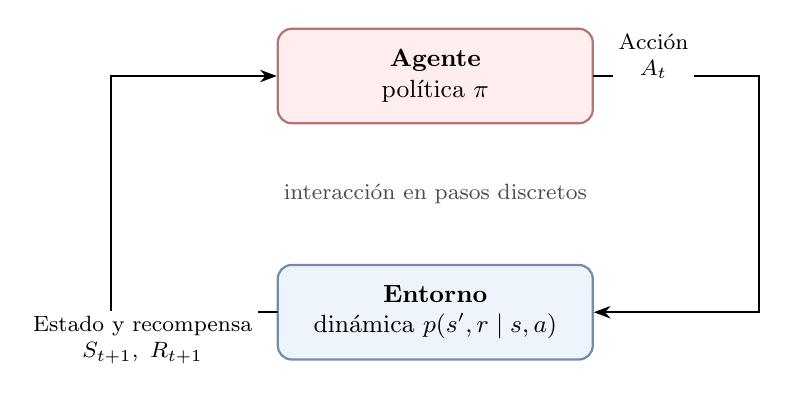
\begin{tikzpicture}[
        bloque/.style={rectangle, rounded corners=5pt, thick, align=center,
            minimum width=4.0cm, minimum height=1.2cm, font=\small},
        bloqueAgente/.style={bloque, draw=colAgente!70!black, fill=colAgente!20},
        bloqueEntorno/.style={bloque, draw=colEntorno!70!black, fill=colEntorno!20},
        flecha/.style={-{Stealth[length=6pt]}, thick, line cap=round},
        etiqueta/.style={font=\footnotesize, fill=white, inner sep=2pt, align=center}
    ]
        \node[bloqueAgente] (agente) at (0, 1.5) {\textbf{Agente}\\pol\'{i}tica $\pi$};
        \node[bloqueEntorno] (entorno) at (0, -1.5) {\textbf{Entorno}\\din\'{a}mica $p(s', r \mid s, a)$};

        \draw[flecha] (agente.east) -- ++(2.1, 0) |- (entorno.east);
        \node[etiqueta, anchor=west] at (2.25, 1.75) {Acci\'{o}n\\$A_t$};

        \draw[flecha] (entorno.west) -- ++(-2.1, 0) |- (agente.west);
        \node[etiqueta, anchor=east] at (-2.25, -1.85) {Estado y recompensa\\$S_{t+1},\ R_{t+1}$};

        \node[font=\footnotesize, text=black!70] at (0, 0) {interacci\'{o}n en pasos discretos};
    \end{tikzpicture}
    \caption{Interacción agente-entorno en un proceso de decisión de Markov \cite{suttonRL}.}
    \label{fig:agent_env_interaction}
\end{figure}

De forma compacta, un MDP finito queda caracterizado por la tupla $\langle \mathcal{S}, \mathcal{A}, P, R, \gamma \rangle$, donde $\mathcal{S}$ es el espacio de estados, $\mathcal{A}$ el espacio de acciones, $P$ la dinámica de transición probabilística, $R$ la función de recompensa y $\gamma \in [0,1)$ el factor de descuento.

La dinámica del entorno queda definida por la función $p(s', r \mid s, a)$, que especifica la probabilidad condicional conjunta de observar el próximo estado $s'$ y la recompensa $r$ al ejecutar la acción $a$ en el estado $s$:
\begin{equation}
p(s', r \mid s, a) \doteq \Pr\{S_{t+1} = s', R_{t+1} = r \mid S_t = s, A_t = a\}
\end{equation}
donde $S_t \in \mathcal{S}$ representa el estado en el instante $t$, $A_t \in \mathcal{A}$ es la acción seleccionada, $R_{t+1} \in \mathbb{R}$ es la recompensa escalar recibida y $S_{t+1} \in \mathcal{S}$ es el nuevo estado resultante.

La propiedad de Markov establece que, dado el estado y la acción actuales, la distribución del próximo estado y recompensa no depende explícitamente de la historia completa de estados y acciones anteriores. En otras palabras, el estado debe contener toda la información relevante del pasado para predecir la evolución futura del proceso \cite{suttonRL}.

Una suposición habitual del MDP es que el agente observa un estado suficientemente informativo del entorno. Sin embargo, en muchas aplicaciones reales el agente solo recibe observaciones parciales o ruidosas. En estos casos, el marco se generaliza a un Proceso de Decisión de Markov Parcialmente Observable (POMDP), donde el historial de observaciones puede ser necesario para inferir el estado subyacente \cite{marlbook}.

Para formalizar la meta de maximizar la recompensa a largo plazo se define el retorno descontado $G_t$, que incorpora un factor $\gamma \in [0,1)$ para ponderar la importancia de las recompensas futuras \cite{suttonRL}:
\begin{equation}
G_t \doteq R_{t+1} + \gamma R_{t+2} + \gamma^2 R_{t+3} + \dots = \sum_{k=0}^{\infty} \gamma^k R_{t+k+1}
\end{equation}
donde $G_t$ representa la suma acumulada descontada de recompensas futuras a partir del instante $t$, y $\gamma$ es el factor de descuento. Un valor de $\gamma$ cercano a cero prioriza recompensas inmediatas, mientras que un valor cercano a uno otorga un peso significativo a recompensas futuras de largo plazo \cite{marlbook}.

\subsection{Métodos Basados en Valor y Basados en Política}

Los algoritmos de RL pueden agruparse, a grandes rasgos, en métodos basados en valor y métodos basados en política. Esta distinción no agota la taxonomía del campo, pero permite introducir las familias de algoritmos más relevantes para este trabajo.

En los \textit{métodos basados en valor}, la estrategia consiste en estimar qué tan conveniente es encontrarse en un estado o ejecutar una acción determinada. Esto se formaliza mediante la \textit{función de valor de estado} $v_\pi(s) \doteq \mathbb{E}_\pi[G_t \mid S_t = s]$ y la \textit{función de valor de acción} $q_\pi(s, a) \doteq \mathbb{E}_\pi[G_t \mid S_t = s, A_t = a]$. Ambas funciones satisfacen ecuaciones recursivas conocidas como \textit{ecuaciones de Bellman}, que expresan la relación entre el valor de una situación actual y el valor esperado de sus posibles sucesores \cite{suttonRL}.

Cuando la dinámica del entorno no se conoce completamente, estas funciones pueden estimarse a partir de la experiencia. Los métodos de Diferencia Temporal (\textit{Temporal-Difference}, TD) combinan el muestreo de transiciones reales con actualizaciones basadas en estimaciones previas, mecanismo conocido como \textit{bootstrapping}. Un ejemplo central es \textit{Q-learning}, que actualiza la función de acción-valor hacia una estimación de la función óptima $q_*(s,a)$:
\begin{equation}
Q(S_t, A_t) \leftarrow Q(S_t, A_t) + \alpha \left[ R_{t+1} + \gamma \max_a Q(S_{t+1}, a) - Q(S_t, A_t) \right]
\end{equation}
donde $Q(S_t, A_t)$ es la estimación del valor de la acción $A_t$ en el estado $S_t$, $\alpha \in (0, 1]$ representa la tasa de aprendizaje (\textit{learning rate}), $R_{t+1}$ es la recompensa observada, $\gamma$ es el factor de descuento, y $\max_a Q(S_{t+1}, a)$ estima el valor máximo alcanzable en el siguiente estado $S_{t+1}$.

Por el contrario, los \textit{métodos basados en política} parametrizan directamente la política $\pi(a \mid s, \theta) = \Pr\{A_t = a \mid S_t = s, \theta_t = \theta\}$, donde $\theta \in \mathbb{R}^d$ representa el vector de parámetros ajustables (pesos neuronales). En lugar de derivar la acción exclusivamente de una función de valor, ajustan los parámetros $\theta$ para maximizar una medida de rendimiento escalar $J(\theta)$. Para ello aplican ascenso de gradiente sobre el rendimiento esperado:
\begin{equation}
\theta_{t+1} = \theta_t + \alpha \nabla J(\theta_t)
\end{equation}
donde $\nabla J(\theta_t)$ representa el gradiente de la función de rendimiento respecto a los parámetros de la política. El Teorema del Gradiente de Política (\textit{Policy Gradient Theorem}) proporciona la base teórica para estimar este gradiente sin derivar explícitamente la distribución de estados inducida por la política \cite{suttonRL}. En la práctica, muchos algoritmos modernos combinan ambas ideas mediante arquitecturas actor-crítico: un actor representa la política y un crítico estima valores para guiar sus actualizaciones.

\begin{figure}[H]
    \centering
    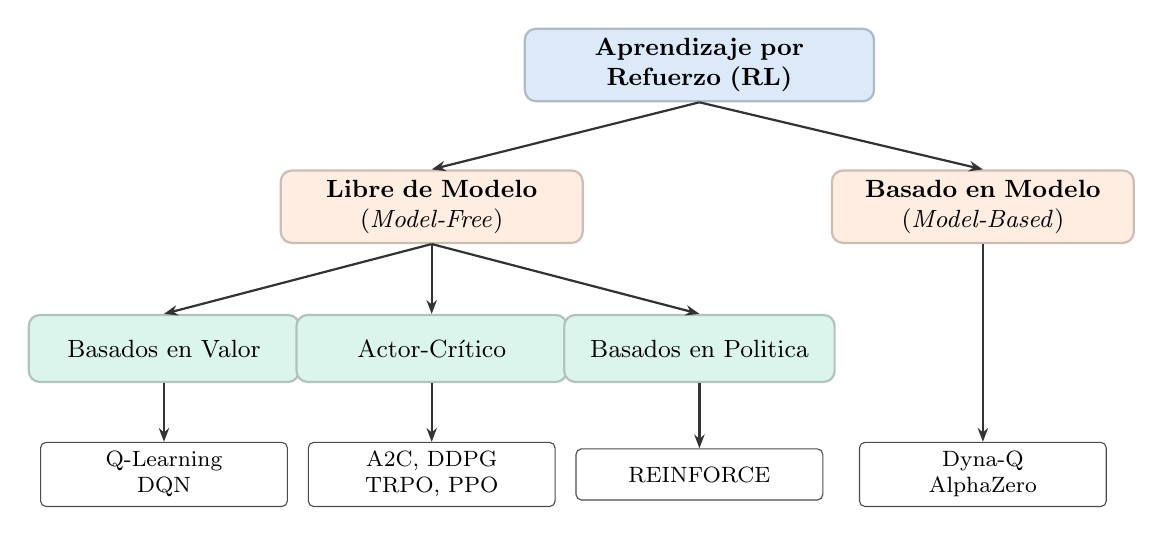
\begin{tikzpicture}[
        box/.style={draw, rounded corners=4pt, align=center, minimum height=0.85cm, font=\small, thick},
        cat1/.style={box, fill=colTaxonomiaNivelUno, draw=colTaxonomiaNivelUno!80!black, text width=4.2cm},
        cat2/.style={box, fill=colTaxonomiaNivelDos, draw=colTaxonomiaNivelDos!80!black, text width=3.6cm},
        cat3/.style={box, fill=colTaxonomiaNivelTres, draw=colTaxonomiaNivelTres!80!black, text width=3.2cm},
        alg/.style={draw=black!70, align=center, fill=white, text width=2.9cm, font=\footnotesize, minimum height=0.65cm, rounded corners=2pt},
        arr/.style={-{Stealth[length=5pt]}, thick, draw=black!80}
    ]

    % Nivel 1
    \node[cat1] (rl) at (0, 0) {\textbf{Aprendizaje por Refuerzo (RL)}};

    % Nivel 2
    \node[cat2] (mf) at (-3.4, -1.8) {\textbf{Libre de Modelo}\\(\textit{Model-Free})};
    \node[cat2] (mb) at (3.6, -1.8) {\textbf{Basado en Modelo}\\(\textit{Model-Based})};

    % Nivel 3 (Ramas de Model-Free)
    \node[cat3] (val) at (-6.8, -3.6) {Basados en Valor};
    \node[cat3] (ac) at (-3.4, -3.6) {Actor-Cr\'{i}tico};
    \node[cat3] (pol) at (0, -3.6) {Basados en Politica};

    % Nivel 4 (Algoritmos)
    \node[alg] (dqn) at (-6.8, -5.2) {Q-Learning\\DQN};
    \node[alg] (ppo) at (-3.4, -5.2) {A2C, DDPG\\TRPO, PPO};
    \node[alg] (reinf) at (0, -5.2) {REINFORCE};
    \node[alg] (alph) at (3.6, -5.2) {Dyna-Q\\AlphaZero};

    % Conexiones Nivel 1 -> Nivel 2
    \draw[arr] (rl.south) -- (mf.north);
    \draw[arr] (rl.south) -- (mb.north);

    % Conexiones Nivel 2 -> Nivel 3
    \draw[arr] (mf.south) -- (val.north);
    \draw[arr] (mf.south) -- (ac.north);
    \draw[arr] (mf.south) -- (pol.north);

    % Conexiones Nivel 3 -> Algoritmos
    \draw[arr] (val.south) -- (dqn.north);
    \draw[arr] (ac.south) -- (ppo.north);
    \draw[arr] (pol.south) -- (reinf.north);

    % Conexiones Nivel 2 -> Algoritmos (Model-Based)
    \draw[arr] (mb.south) -- (alph.north);

    \end{tikzpicture}
    \caption{Taxonomía de algoritmos de Aprendizaje por Refuerzo, enfocada en métodos \textit{Model-Free} (adaptada de OpenAI \textit{Spinning Up} \cite{spinningup}).}
    \label{fig:rl_taxonomy}
\end{figure}

\subsection{Aprendizaje Profundo y Redes Neuronales}

\subsubsection{La Unidad Neuronal y Redes \textit{Feedforward}}

En problemas de control complejos, los métodos tabulares se vuelven impracticables debido a las restricciones de memoria y cómputo que impone la maldición de la dimensionalidad \cite{suttonRL}. La aproximación de funciones soluciona esta limitación al representar funciones mediante una forma parametrizada, permitiendo que el aprendizaje en un estado se generalice a otros estados con características similares. El aprendizaje profundo (\textit{Deep Learning}) emplea redes neuronales artificiales como aproximadores de funciones continuas y no lineales \cite{marlbook}.

El componente básico de estas arquitecturas es la unidad neuronal individual. Computacionalmente, una neurona en una capa $k$ ejecuta dos operaciones secuenciales sobre el vector de características de entrada $\mathbf{x}$. Primero, calcula una combinación lineal utilizando un vector de pesos $\mathbf{w}$ y un sesgo (\textit{bias}) escalar $b$. Luego, el resultado se somete a una función de activación no lineal $g_k$:
\begin{equation}
    f_{k,u}(\mathbf{x}; \theta_k^u) = g_k(\mathbf{w}^\top \mathbf{x} + b)
\end{equation}
donde $\mathbf{x} \in \mathbb{R}^d$ es el vector de entrada, $\mathbf{w} \in \mathbb{R}^d$ representa los pesos asociativos, $b \in \mathbb{R}$ es el sesgo, y $g_k$ es la función de activación diferenciable. La inclusión de una función de activación no lineal es estrictamente necesaria; componer múltiples capas sin funciones no lineales resultaría analíticamente en una simple transformación lineal, anulando la capacidad de representación de la red \cite{marlbook}. Entre las opciones no lineales más comunes destacan ReLU (Unidad Lineal Rectificada, $g(z) = \max(0, z)$), \textit{leaky} ReLU ($g(z) = \max(\alpha z, z)$ con $\alpha \ll 1$) y Tanh (tangente hiperbólica, comprimiendo las salidas en $[-1, 1]$).

Las redes neuronales de propagación hacia adelante (\textit{feedforward} o perceptrones multicapa) estructuran estas unidades en secuencias de múltiples capas: una capa de entrada, capas intermedias u ocultas, y una capa de salida. La computación de una capa entera se puede vectorizar:
\begin{equation}
    \mathbf{h}_k = g_k(\mathbf{W}_k^\top \mathbf{x}_{k-1} + \mathbf{b}_k)
\end{equation}
donde $\mathbf{W}_k$ es la matriz de pesos de la capa $k$, $\mathbf{x}_{k-1}$ es la salida activada de la capa previa y $\mathbf{b}_k$ es el vector de sesgos. El Teorema de Aproximación Universal establece que una red con una única capa oculta suficientemente ancha puede aproximar cualquier función continua; sin embargo, arquitecturas más profundas logran una mejor generalización y una extracción jerárquica de características progresivamente más abstractas \cite{marlbook, suttonRL}.

\subsubsection{El Proceso de Optimización}

Dado que las redes neuronales carecen de una solución de forma cerrada, sus parámetros $\theta$ se ajustan utilizando métodos de optimización iterativa. El proceso se fundamenta en tres componentes técnicos \cite{marlbook}:

\begin{itemize}
    \item \textbf{Función de Pérdida (\textit{Loss Function}):} Un objetivo matemático diferenciable $\mathcal{L}(\theta)$ que cuantifica la discrepancia entre las predicciones de la red y los valores objetivo. Frecuentemente se emplea el Error Cuadrático Medio (MSE).
    \item \textbf{Descenso de Gradiente:} El optimizador actualiza los parámetros moviéndose en la dirección del gradiente negativo $-\nabla_\theta \mathcal{L}(\theta)$, ponderado por una tasa de aprendizaje $\alpha$. En la práctica se utiliza el Descenso de Gradiente por Mini-lotes (\textit{Mini-batch Gradient Descent}), que muestrea un subconjunto aleatorio de datos para ofrecer un equilibrio óptimo entre la estabilidad del gradiente y el costo computacional. Optimizadores modernos como Adam adaptan dinámicamente las tasas de aprendizaje para acelerar la convergencia.
    \item \textbf{Retropropagación (\textit{Backpropagation}):} Para que el descenso de gradiente sea posible en arquitecturas profundas, es necesario computar las derivadas parciales de la función de pérdida respecto a cada parámetro. El algoritmo de \textit{backpropagation} logra esto aplicando eficientemente la regla de la cadena de derivadas, propagando los gradientes desde la capa de salida hacia las capas de entrada.
\end{itemize}

\subsection{Aprendizaje por Refuerzo Profundo (DRL)}

El Aprendizaje por Refuerzo Profundo (DRL) combina los algoritmos de RL con la capacidad de generalización del aprendizaje profundo. Esta integración es fundamental cuando los espacios de estado son continuos o de alta dimensionalidad, donde es estadísticamente improbable que un agente visite el mismo estado múltiples veces. Sin embargo, el DRL exige aproximadores robustos capaces de procesar flujos de datos correlacionados temporalmente y de rastrear objetivos no estacionarios \cite{marlbook}.

\subsubsection{El Problema de la Tríada Mortal (\textit{Deadly Triad})}

La aplicación directa de redes neuronales al aprendizaje por refuerzo introduce vulnerabilidades analíticas. Sutton y Barto \cite{suttonRL} establecen que la inestabilidad de los parámetros y la divergencia de los valores están garantizadas matemáticamente si un algoritmo combina simultáneamente tres elementos fundamentales:

\begin{itemize}
    \item \textbf{Aproximación de Funciones:} Uso de aproximadores potentes y escalables, como las redes neuronales, que extienden el aprendizaje generalizando a través del espacio de estados.
    \item \textbf{\textit{Bootstrapping}:} La práctica de actualizar estimaciones de valor apoyándose en otras estimaciones aprendidas previamente (como en los métodos TD), en lugar de esperar la consecución de retornos reales completos.
    \item \textbf{Entrenamiento \textit{Off-Policy}:} Optimizar la función de valor utilizando una distribución de datos o transiciones generadas por una política de comportamiento distinta a la política objetivo que se desea evaluar o mejorar.
\end{itemize}

El análisis de la Tríada Mortal argumenta que es fácticamente imposible prescindir de cualquiera de estos tres vértices en sistemas de control escalables \cite{suttonRL}. Renunciar a la aproximación de funciones restringiría el control a problemas tabulares diminutos. Descartar el \textit{bootstrapping} mitigaría la inestabilidad, pero paralizaría la eficiencia de datos y la viabilidad computacional al requerir almacenar secuencias episódicas enteras. Finalmente, sacrificar el aprendizaje \textit{off-policy} anularía la capacidad del agente de aprender de forma concurrente múltiples modelos predictivos a partir de un único flujo de experiencia. Por consiguiente, resulta imperativo tolerar la Tríada Mortal e incorporar mitigaciones algorítmicas estructurales.

\subsubsection{\textit{Deep Q-Networks} (DQN)}

En los métodos basados en valor, DRL sustituye la tabla clásica por una red neuronal $Q(s, a; \theta)$. En espacios de acción discretos, el algoritmo \textit{Deep Q-Networks} (DQN) procesa el estado $s$ como vector de entrada y computa simultáneamente las estimaciones de valor para todas las acciones en su capa de salida \cite{marlbook, mnih2015}.

La inestabilidad descrita por la Tríada Mortal se manifiesta en DQN como el ``problema del blanco móvil'': al generalizar, una actualización que incrementa el valor de un estado modifica de forma inadvertida los valores de otros estados. Si además las secuencias de entrenamiento presentan una alta correlación temporal, la red sufre de olvido catastrófico, sobreajustándose a la experiencia más reciente. Para lograr convergencia, DQN introduce dos innovaciones estructurales imperativas \cite{marlbook}:

\begin{itemize}
    \item \textbf{Redes Objetivo (\textit{Target Networks}):} Se emplea una red neuronal secundaria separada cuyos parámetros $\theta^-$ se congelan temporalmente. Esta red se utiliza exclusivamente para calcular los valores objetivo en el error TD, amortiguando las oscilaciones y estabilizando el blanco de aprendizaje.
    \item \textbf{Búferes de Repetición (\textit{Replay Buffers}):} Se almacenan las transiciones históricas del agente $(s, a, r, s')$. El entrenamiento se realiza extrayendo mini-lotes aleatorios de esta memoria, lo cual destruye la correlación temporal intrínseca de los procesos de decisión de Markov y estabiliza la varianza del gradiente.
\end{itemize}

La función de pérdida minimizada por DQN es:
\begin{equation}
\mathcal{L}(\theta) = \mathbb{E}_{(s_j, a_j, r_j, s_{j+1}) \sim \mathcal{D}} \left[ \left( \underbrace{r_j + \gamma \max_{a'} \hat{Q}(s_{j+1}, a'; \theta^{-})}_{\text{Valor Objetivo de TD}} - \underbrace{Q(s_j, a_j; \theta)}_{\text{Predicción Actual}} \right)^2 \right]
\end{equation}
donde $\mathcal{D}$ es el búfer de repetición de experiencias, $(s_j, a_j, r_j, s_{j+1})$ representa una transición muestreada, $\theta$ indica los parámetros de la red $Q$ actual y $\theta^-$ representa los parámetros congelados de la red objetivo.

\begin{algorithm}[H]
\caption{Algoritmo \textit{Deep Q-Networks} (DQN) con \textit{Replay Buffer}}
\label{alg:dqn}
\begin{algorithmic}[1]
\State Inicializar la memoria de repetición $\mathcal{D}$ con capacidad $N$
\State Inicializar la red de acción-valor $Q$ con pesos aleatorios $\theta$
\State Inicializar la red objetivo $\hat{Q}$ con pesos $\theta^- = \theta$
\For{episodio $= 1$ hasta $M$}
    \State Inicializar secuencia y obtener estado inicial $s_1$
    \For{$t = 1$ hasta $T$}
        \State Seleccionar una acción $a_t$ mediante política $\epsilon$-greedy a partir de $Q(s_t, a; \theta)$
        \State Ejecutar acción $a_t$, observar recompensa $r_t$ y siguiente estado $s_{t+1}$
        \State Almacenar transición $(s_t, a_t, r_t, s_{t+1})$ en $\mathcal{D}$
        \State Muestrear un minilote aleatorio de transiciones $(s_j, a_j, r_j, s_{j+1})$ desde $\mathcal{D}$
        \State Calcular objetivo $y_j = \begin{cases} r_j & \text{si } s_{j+1} \text{ es terminal} \\ r_j + \gamma \max_{a'} \hat{Q}(s_{j+1}, a'; \theta^-) & \text{en otro caso} \end{cases}$
        \State Realizar un paso de descenso de gradiente respecto a la pérdida $(y_j - Q(s_j, a_j; \theta))^2$ para ajustar $\theta$
        \State Cada $C$ pasos, sincronizar la red objetivo: $\theta^- \leftarrow \theta$
    \EndFor
\EndFor
\end{algorithmic}
\end{algorithm}

\subsubsection{Aproximación de Políticas, Función de Ventaja y \textit{Policy Gradient}}

Como alternativa a derivar la política de forma indirecta a partir de una función de valor (como en DQN), DRL permite parametrizar directamente la política del agente mediante una red neuronal $\pi(a|s; \theta)$ \cite{marlbook}.

Para cuantificar el desempeño marginal de una acción tomada en un estado específico respecto a la expectativa promedio de la política, se define la \textbf{Función de Ventaja} (\textit{Advantage Function}) $A^\pi(s, a)$ \cite{suttonRL}:
\begin{equation}
    A^\pi(s, a) \doteq Q^\pi(s, a) - V^\pi(s)
\end{equation}
donde $Q^\pi(s, a)$ representa el retorno esperado al tomar la acción $a$ en el estado $s$ bajo la política $\pi$, y $V^\pi(s)$ es el valor promedio de estado. Conceptualmente, la ventaja mide cuánto mejor ($A^\pi(s, a) > 0$) o peor ($A^\pi(s, a) < 0$) resulta la acción $a$ en comparación con el desempeño medio del agente en el estado $s$.

En arquitecturas actor-crítico, la ventaja se estima habitualmente mediante la Estimación Generalizada de la Ventaja (\textit{Generalized Advantage Estimation}, GAE) desarrollada por Schulman et al. \cite{schulman2015high}:
\begin{equation}
    \hat{A}_t^{\text{GAE}(\gamma, \lambda)} \doteq \sum_{l=0}^{\infty} (\gamma \lambda)^l \delta_{t+l}^V
\end{equation}
donde $\delta_t^V = R_{t+1} + \gamma V(S_{t+1}) - V(S_t)$ representa el error de diferencia temporal (TD) estimado por la red del crítico $V$, $\gamma \in [0, 1)$ es el factor de descuento y $\lambda \in [0, 1]$ es el hiperparámetro de suavizado GAE que equilibra el sesgo y la varianza del estimador.

En lugar de minimizar un error cuadrático de predicción, la optimización paramétrica del actor se rige por el Teorema del Gradiente de Política (\textit{Policy Gradient Theorem}), que establece la actualización de los parámetros $\theta$ ascendiendo por el gradiente del rendimiento esperado \cite{suttonRL, schulman2015high}:
\begin{equation}
    \nabla_\theta J(\theta) = \hat{\mathbb{E}}_t \left[ \nabla_\theta \log \pi_\theta(A_t \mid S_t) \hat{A}_t \right]
\end{equation}
donde $\nabla_\theta J(\theta)$ representa el gradiente del desempeño esperado, $\pi_\theta(A_t \mid S_t)$ es la probabilidad otorgada a la acción ejecutada $A_t$ en el estado $S_t$, y $\hat{A}_t$ es la ventaja estimada. Esta formulación incrementa la probabilidad de elegir acciones con ventaja positiva ($\hat{A}_t > 0$) y reduce la probabilidad de aquellas con ventaja negativa.

\subsubsection{\textit{Proximal Policy Optimization} (PPO) y Mejora Monótona}

Una dificultad conocida de los métodos de gradiente de política tradicionales (como REINFORCE o A2C) es su sensibilidad a la tasa de aprendizaje: actualizaciones de parámetros con pasos demasiado grandes pueden modificar la distribución de la política de forma abrupta, provocando un colapso catastrófico del desempeño del cual el agente raramente se recupera.

Para resolver esta vulnerabilidad, Kakade y Langford \cite{kakade2002approximately} y Schulman et al. (TRPO \cite{schulman2015trust}) formalizaron el principio de \textbf{Mejora Monótona de la Política} (\textit{Monotonic Policy Improvement}). Este principio garantiza matemáticamente que en cada iteración de optimización $k$, el retorno esperado del agente es monótonamente no decreciente:
\begin{equation}
    J(\pi_{k+1}) \ge J(\pi_k)
\end{equation}
donde $J(\pi_k)$ representa el desempeño esperado de la política en la iteración $k$, y $J(\pi_{k+1})$ es el desempeño esperado tras actualizar sus parámetros. Mientras que TRPO logra esta garantía imponiendo una restricción severa sobre la divergencia Kullback-Leibler (KL) mediante optimización cuadrática de segundo orden, \textit{Proximal Policy Optimization} (PPO) \cite{schulman2017ppo} aproxima este comportamiento mediante un objetivo sustituto recortado (\textit{clipped surrogate objective}) computable mediante descenso de gradiente de primer orden.

Dada la razón de probabilidad entre la política actual y la anterior:
\begin{equation}
r_t(\theta) \doteq \frac{\pi_\theta(a_t \mid s_t)}{\pi_{\theta_{\text{old}}}(a_t \mid s_t)}
\end{equation}
donde $\pi_\theta(a_t \mid s_t)$ es la probabilidad de la acción $a_t$ bajo los nuevos parámetros $\theta$, y $\pi_{\theta_{\text{old}}}(a_t \mid s_t)$ es la probabilidad registrada durante la recolección del lote, PPO maximiza el siguiente objetivo recortado:
\begin{equation}
L^{\text{CLIP}}(\theta) = \hat{\mathbb{E}}_t \left[ \min\left( r_t(\theta) \hat{A}_t, \, \text{clip}(r_t(\theta), 1-\epsilon, 1+\epsilon) \hat{A}_t \right) \right]
\end{equation}
donde $\epsilon > 0$ es un hiperparámetro de recorte (típicamente $\epsilon \approx 0.1\text{--}0.2$), y $\text{clip}(r, 1-\epsilon, 1+\epsilon)$ acota la razón $r$ al intervalo $[1-\epsilon, 1+\epsilon]$. El operador $\min$ toma el valor más pesimista entre la ventaja ponderada simple y la ventaja recortada, eliminando el incentivo a realizar actualizaciones que modifiquen excesivamente la política si la ventaja es positiva, y acotando la penalización si la ventaja es negativa.

En la práctica, la función objetivo completa de PPO combina el término de política, la pérdida de ajuste del crítico y un término de entropía para favorecer la exploración:
\begin{equation}
\mathcal{L}^{\text{PPO}}(\theta, \phi) = \hat{\mathbb{E}}_t \left[ L^{\text{CLIP}}(\theta) - c_1 \left( V_\phi(s_t) - V_t^{\text{target}} \right)^2 + c_2 S[\pi_\theta](s_t) \right]
\end{equation}
donde $\phi$ representa los parámetros de la red del crítico $V_\phi$, $V_t^{\text{target}}$ son los retornos observados objetivo, $S[\pi_\theta]$ denota la entropía de la distribución de la política, y $c_1, c_2 > 0$ son coeficientes de ponderación escalar.

PPO es un algoritmo *on-policy* caracterizado por su estabilidad y simplicidad. En esta tesina, su importancia no se limita a su rol individual, sino que constituye la base algorítmica sobre la cual se estructuran tanto el *baseline* independiente (IPPO) como las extensiones cooperativas multi-agente (MAPPO y HAPPO).

\begin{algorithm}[H]
\caption{Algoritmo \textit{Proximal Policy Optimization} (PPO) - Variante \textit{Actor-Critic}}
\label{alg:ppo}
\begin{algorithmic}[1]
\State Inicializar parámetros de política (actor) $\theta$ y función de valor (crítico) $\phi$
\For{iteración $= 1, 2, \dots$}
    \State Recolectar un conjunto de trayectorias $\mathcal{D}_k = \{\tau_i\}$ ejecutando la política actual $\pi_{\theta}$ en el entorno
    \State Calcular los valores del crítico $V_\phi(s)$ y las estimaciones de ventaja $\hat{A}_t^{\text{GAE}}$
    \State Optimizar el objetivo $L^{\text{CLIP}}(\theta)$ respecto a $\theta$ durante $K$ épocas (\textit{epochs}) sobre minilotes de $\mathcal{D}_k$
    \State Optimizar la función de pérdida del crítico $L^{\text{VF}}(\phi) = (V_\phi(s_t) - \hat{V}_t)^2$ respecto a $\phi$
\EndFor
\end{algorithmic}
\end{algorithm}

\section[Aprendizaje por Refuerzo Multi-Agente (MARL)]{Aprendizaje por Refuerzo \\ Multi-Agente (MARL)}

El aprendizaje por refuerzo multi-agente (\textit{Multi-Agent Reinforcement Learning}, MARL) generaliza los principios del RL hacia sistemas donde múltiples entidades aprenden e interactúan simultáneamente en un entorno compartido \cite{marlbook}. A diferencia del caso individual, las acciones de cada agente modifican el estado global del sistema, lo que induce una dinámica no estacionaria desde la perspectiva local de cualquier participante. En el contexto de sistemas dinámicos cooperativos, múltiples controladores coordinan sus decisiones para optimizar un objetivo común.

\subsection{Fundamentos Teóricos: Juegos Estocásticos, Equilibrio de Nash y Dec-POMDP}

La formalización matemática de los entornos multi-agente requiere extender el MDP individual incorporando nociones de la Teoría de Juegos. El modelo matemático fundamental para representar decisiones secuenciales con múltiples participantes es el Juego Estocástico o Juego Markoviano (\textit{Stochastic Game} o \textit{Markov Game}), introducido por Shapley \cite{shapley1953stochastic} y adaptado al aprendizaje por refuerzo por Albrecht et al. \cite{marlbook}.

Un Juego Estocástico para $n$ agentes se define mediante la tupla:
\begin{equation}
    \langle \mathcal{N}, \mathcal{S}, \{ \mathcal{A}_i \}_{i=1}^n, P, \{ R_i \}_{i=1}^n, \gamma \rangle
\end{equation}
donde $\mathcal{N} = \{1, \dots, n\}$ representa el conjunto de agentes, $\mathcal{S}$ es el espacio de estados globales, $\mathcal{A}_i$ es el espacio de acciones del agente $i$, $P(s' \mid s, \mathbf{a})$ representa la función de transición de estados condicionada a la acción conjunta $\mathbf{a} = (a_1, \dots, a_n) \in \boldsymbol{\mathcal{A}} \equiv \mathcal{A}_1 \times \dots \times \mathcal{A}_n$, y $R_i(s, \mathbf{a})$ representa la función de recompensa asignada al agente $i$. En un entorno estrictamente cooperativo, todos los agentes comparten exactamente la misma señal de recompensa ($R_1 = R_2 = \dots = R_n = R$), de modo que el objetivo de cada agente es maximizar el retorno global esperado del sistema.

En el marco de la Teoría de Juegos, la solución teórica a la que aspiran los algoritmos de MARL es el \textbf{Equilibrio de Nash} \cite{marlbook}. Una política conjunta $\boldsymbol{\pi}^* = (\pi_1^*, \dots, \pi_n^*)$ constituye un Equilibrio de Nash si ningún agente $i \in \mathcal{N}$ puede incrementar unilateralmente su retorno esperado desviándose de su política $\pi_i^*$, asumiendo que los demás agentes mantienen sus políticas fijas en $\boldsymbol{\pi}_{-i}^*$:
\begin{equation}
    J(\pi_i, \boldsymbol{\pi}_{-i}^*) \le J(\pi_i^*, \boldsymbol{\pi}_{-i}^*), \quad \forall \pi_i \in \Pi_i, \quad \forall i \in \mathcal{N}
\end{equation}
donde $\boldsymbol{\pi}^* = (\pi_1^*, \dots, \pi_n^*)$ es la combinación de políticas individuales en equilibrio, $\pi_i$ representa cualquier política alternativa ejecutable por el agente $i$, $\Pi_i$ denota el espacio de políticas válidas del agente $i$, y $\boldsymbol{\pi}_{-i}^* = (\pi_1^*, \dots, \pi_{i-1}^*, \pi_{i+1}^*, \dots, \pi_n^*)$ es el vector de políticas fijas de todos los demás agentes excepto el agente $i$. En términos sencillos, un Equilibrio de Nash representa un punto de convergencia donde ninguna entidad tiene un incentivo individual para alterar unilateralmente su estrategia.

En escenarios reales de control distribuido, ningún agente dispone de visibilidad completa del estado global del sistema. Cada participante recopila información únicamente de sus sensores locales. Por consiguiente, los entornos cooperativos multi-agente con observabilidad parcial se formalizan matemáticamente mediante el marco de los Procesos de Decisión de Markov Parcialmente Observables Descentralizados (Dec-POMDP) \cite{marlbook, decpomdp-survey}.

Un Dec-POMDP para $n$ agentes se define como una tupla:
\begin{equation}
    \langle \mathcal{N}, \mathcal{S}, \{ \mathcal{A}_i \}_{i=1}^n, P, R, \{ \Omega_i \}_{i=1}^n, O, \gamma \rangle
\end{equation}
donde $\Omega_i$ denota el conjunto de observaciones individuales del agente $i$, regidas por la función de observación probabilística $O(o_1, \dots, o_n \mid s', \mathbf{a}) = \Pr\{O_1 = o_1, \dots, O_n = o_n \mid S' = s', \mathbf{A} = \mathbf{a}\}$. En este esquema, cada agente $i$ basa sus decisiones únicamente en su historial u observación local $o_i \in \Omega_i$, con el propósito de aprender una política descentralizada $\pi_i(a_i \mid o_i)$ que, al combinarse con las políticas de los demás agentes en la política conjunta $\boldsymbol{\pi} = (\pi_1, \dots, \pi_n)$, maximice el retorno acumulado conjunto del sistema \cite{decpomdp-survey}.

\begin{figure}[H]
    \centering
    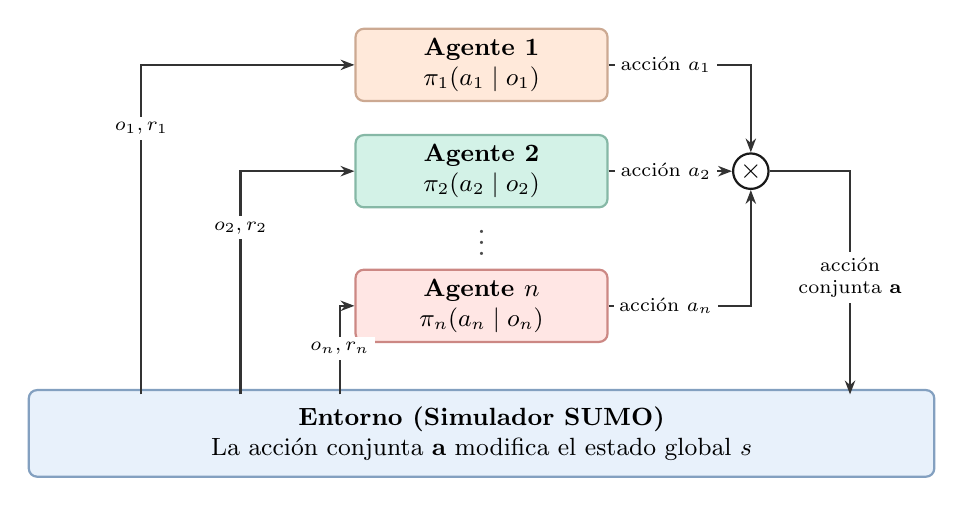
\begin{tikzpicture}[
        scale=0.9,
        bloque/.style={rectangle, thick, align=center, font=\small, draw=black!80, rounded corners=3pt},
        bloqueAg1/.style={bloque, fill=catMelocoton!50, draw=catMelocoton!80!black, minimum width=3.2cm, minimum height=0.9cm},
        bloqueAg2/.style={bloque, fill=colInterfaz!50, draw=colInterfaz!80!black, minimum width=3.2cm, minimum height=0.9cm},
        bloqueAgn/.style={bloque, fill=colAgente!30, draw=colAgente!80!black, minimum width=3.2cm, minimum height=0.9cm},
        bloqueEntorno/.style={bloque, fill=colEntorno!25, draw=colEntorno!80!black, minimum width=11.5cm, minimum height=1.1cm},
        flecha/.style={-{Stealth[length=5pt]}, thick, draw=black!80},
        etiquetaSinFondo/.style={font=\scriptsize, align=center, inner sep=2pt, fill=white},
        mixer/.style={circle, draw=black!90, thick, inner sep=0pt, minimum size=0.45cm}
    ]
        % Entorno
        \node[bloqueEntorno] (entorno) at (0, 0) {\textbf{Entorno (Simulador SUMO)}\\La acción conjunta $\mathbf{a}$ modifica el estado global $s$};

        % Agentes (Apilados verticalmente de forma compacta)
        \node[bloqueAgn] (agenten) at (0, 1.8) {\textbf{Agente $n$}\\$\pi_n(a_n \mid o_n)$};
        \node[font=\large, text=black!70] (dots) at (0, 2.8) {$\vdots$};
        \node[bloqueAg2] (agente2) at (0, 3.7) {\textbf{Agente 2}\\$\pi_2(a_2 \mid o_2)$};
        \node[bloqueAg1] (agente1) at (0, 5.2) {\textbf{Agente 1}\\$\pi_1(a_1 \mid o_1)$};
        
        % OBSERVACIONES (Salen del entorno y suben por la izquierda)
        \draw[flecha] (-4.8, 0.55) |- (agente1.west);
        \node[etiquetaSinFondo] at (-4.8, 4.3) {$o_1, r_1$};
        
        \draw[flecha] (-3.4, 0.55) |- (agente2.west);
        \node[etiquetaSinFondo] at (-3.4, 2.9) {$o_2, r_2$};

        \draw[flecha] (-2.0, 0.55) |- (agenten.west);
        \node[etiquetaSinFondo] at (-2.0, 1.2) {$o_n, r_n$};

        % ACCIONES (Salen de los agentes por la derecha hacia el mezclador)
        \node[mixer] (mix) at (3.8, 3.7) {$\times$};
        
        \draw[flecha] (agente1.east) -| (mix.north);
        \node[etiquetaSinFondo] at (2.6, 5.2) {acción $a_1$};

        \draw[flecha] (agente2.east) -- (mix.west);
        \node[etiquetaSinFondo] at (2.6, 3.7) {acción $a_2$};

        \draw[flecha] (agenten.east) -| (mix.south);
        \node[etiquetaSinFondo] at (2.6, 1.8) {acción $a_n$};

        % Acción conjunta al entorno
        \draw[flecha] (mix.east) -| (5.2, 0.55);
        \node[etiquetaSinFondo] at (5.2, 2.2) {acción\\conjunta $\mathbf{a}$};
    \end{tikzpicture}
    \caption{Interacción Agente-Entorno en un esquema MARL cooperativo. Cada semáforo emite una acción local ($a_i$) formando una acción conjunta ($\mathbf{a}$) que modifica el estado global del entorno de tráfico.}
    \label{fig:marl_interaction}
\end{figure}

\subsection{Desafíos Fundamentales en MARL}

La aplicación práctica de métodos de aprendizaje por refuerzo en escenarios multi-agente enfrenta obstáculos analíticos y computacionales significativos que no existen en el caso individual \cite{marlbook}. A medida que aumenta el número de agentes, el espacio de acciones conjunto $\boldsymbol{\mathcal{A}}$ crece de forma exponencial con el número de agentes ($|\boldsymbol{\mathcal{A}}| = \prod_{i=1}^n |\mathcal{A}_i|$), lo que se conoce como la maldición de la dimensionalidad multi-agente. Sin embargo, los desafíos teóricos más severos radican en la dinámica propia de la interacción:

\begin{itemize}
    \item \textbf{No Estacionariedad:} Desde la perspectiva de un agente individual $i$, las políticas de los demás agentes actúan como parte de la dinámica de transición del entorno. Como todos los agentes aprenden y adaptan sus pesos neuronales de manera concurrente, la función de transición efectiva percibida localmente por el agente $i$:
    \begin{equation}
        \mathcal{P}_i(s' \mid s, a_i) = \sum_{\mathbf{a}_{-i}} P(s' \mid s, a_i, \mathbf{a}_{-i}) \boldsymbol{\pi}_{-i}(\mathbf{a}_{-i} \mid s)
    \end{equation}
    cambia de forma continua a lo largo del entrenamiento. Aquí $\mathbf{a}_{-i}$ representa las acciones conjuntas del resto de los agentes y $\boldsymbol{\pi}_{-i}$ sus respectivas políticas. Esta co-adaptación rompe la Propiedad de Markov base desde la perspectiva local e invalida las garantías de convergencia de los algoritmos de agente único \cite{marlbook,foerster2017}.
    \item \textbf{Observabilidad Parcial:} Dado el modelo Dec-POMDP inherente, la falta de telemetría global restringe la visión de cada agente a variables puramente locales. Esto introduce estocasticidad e incertidumbre en la varianza de los gradientes evaluados, dificultando la estimación precisa de las funciones de valor.
    \item \textbf{Asignación de Crédito Multi-Agente (\textit{Credit Assignment}):} En juegos de recompensa común, resulta complejo discernir analíticamente la contribución o el demérito marginal que la acción de un agente aislado produjo sobre el desempeño sistémico global. Una decisión local subóptima podría recibir un refuerzo positivo si el resto del sistema operó de manera sumamente eficiente, sesgando las actualizaciones de la política \cite{marlbook}.
\end{itemize}

\subsection{Paradigmas de Entrenamiento y Ejecución}

Para abordar estas patologías en escenarios Dec-POMDP, la literatura clasifica los algoritmos en función de cómo fluye la información durante el proceso de optimización. Se distinguen fundamentalmente dos enfoques: el Aprendizaje Independiente (\textit{Independent Learning}, IL) y el Entrenamiento Centralizado con Ejecución Descentralizada (\textit{Centralized Training with Decentralized Execution}, CTDE) \cite{ctde_survey, marlbook}.

En el primero, los agentes se entrenan localmente utilizando métodos de agente único, tratando empíricamente al resto de los agentes como parte de la dinámica del entorno. En el segundo, durante la fase de entrenamiento simulado (\textit{offline}), los algoritmos explotan información global privilegiada (historiales conjuntos o concatenación de observaciones) para guiar y estabilizar la optimización de las funciones de valor. Una vez finalizado el entrenamiento, el componente centralizado se descarta y los actores ejecutan políticas condicionadas estrictamente a observaciones locales en tiempo real (\textit{online}).

\subsection{Multi-Agent Deep Reinforcement Learning (MADRL) y Algoritmos Baseline}

La integración de los formalismos Dec-POMDP con la capacidad de aproximación generalizada del aprendizaje profundo ha dado origen al campo del \textit{Multi-Agent Deep Reinforcement Learning} (MADRL) \cite{maddpg, marlbook}. Esta área agrupa los enfoques prevalentes para el control adaptativo de sistemas complejos a gran escala.

En esta investigación, para evaluar rigurosamente el desempeño de las arquitecturas de entrenamiento centralizado (MAPPO y HAPPO), resulta metodológicamente indispensable establecer \textbf{líneas de base} (\textit{baselines}) \textbf{de aprendizaje independiente (IL)}. En los algoritmos independientes, cada coordinador actúa como un agente aislado que ignora la presencia explícita de los demás participantes.

\subsubsection{Aprendizaje Independiente (IL): IDQN e IPPO como Algoritmos Baseline}

\begin{itemize}
    \item \textbf{\textit{Independent DQN} (IDQN) como Baseline Basado en Valor:} Representa la extensión multi-agente más directa de Q-Learning profundo \cite{tampuu2017multiagent}. Su principal vulnerabilidad metodológica radica en que, al ser un algoritmo \textit{off-policy}, depende críticamente del remuestreo de transiciones desde un \textit{Replay Buffer}. En un entorno MARL no estacionario, esas memorias corresponden a configuraciones históricas donde los demás agentes operaban bajo políticas pasadas. Entrenar sobre estos datos obsoletos agrava la inestabilidad descrita por la Tríada Mortal, provocando la divergencia del valor y el colapso del aprendizaje \cite{foerster2017}. En la evaluación experimental de este trabajo, IDQN sirve como \textit{baseline} representativo de los métodos basados en valor independientes.
    \item \textbf{\textit{Independent PPO} (IPPO) como Baseline Basado en Política:} Asigna una instancia del algoritmo PPO a cada agente. A diferencia de IDQN, la literatura ha demostrado empíricamente que IPPO exhibe una mayor robustez técnica frente a la no estacionariedad \cite{de2020independent}. Esta resiliencia se fundamenta en su naturaleza \textit{on-policy}: al descartar memorias pasadas y extraer gradientes únicamente de datos muestreados en proximidad temporal directa con la política conjunta actual, asegura que las actualizaciones respondan a la dinámica vigente del sistema. Adicionalmente, el recorte paramétrico ($\text{clip}$) previene saltos perjudiciales en el espacio de la política. IPPO constituye el \textit{baseline} independiente principal contra el cual se contrastan los algoritmos coordinados.
\end{itemize}

\begin{figure}[H]
    \centering
    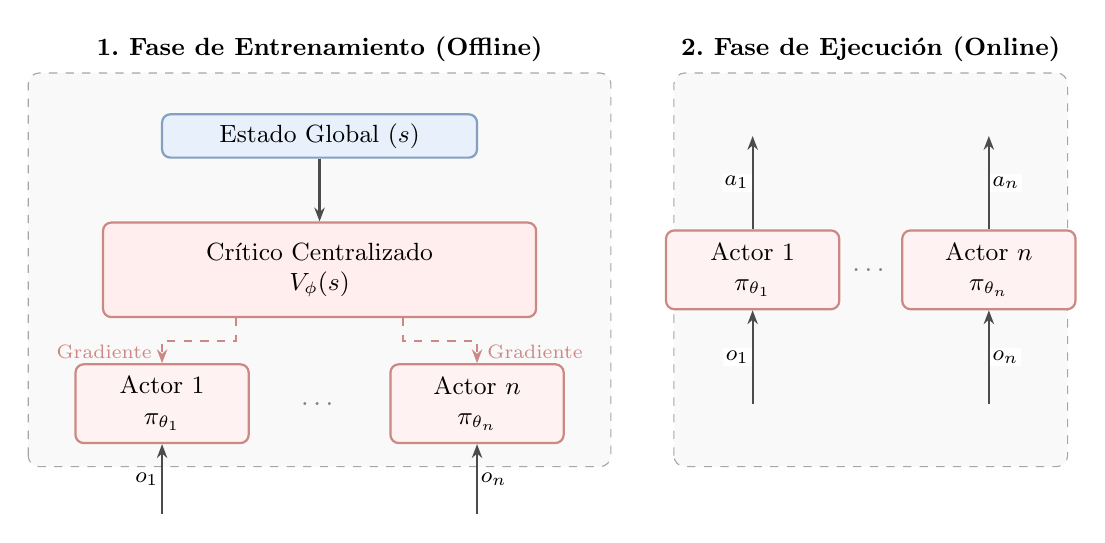
\begin{tikzpicture}[
        box/.style={draw, rounded corners=3pt, thick, align=center, font=\small, fill=white},
        actor/.style={box, draw=colAgente!80!black, fill=colAgente!15, minimum width=2.2cm, minimum height=1cm},
        critic/.style={box, draw=colConflicto, fill=catRosaSalmon!20, minimum width=5.5cm, minimum height=1.2cm},
        arr/.style={-{Stealth[length=5pt]}, thick, draw=black!70},
        lbl/.style={font=\footnotesize, fill=white, inner sep=1pt}
    ]
        % --- FASE DE ENTRENAMIENTO ---
        \node[font=\bfseries\small] at (-0.5, 4.3) {1. Fase de Entrenamiento (Offline)};
        \draw[dashed, draw=gray!70, rounded corners, fill=gray!5] (-4.2, -1) rectangle (3.2, 4.0);

        % Estado Global
        \node[box, fill=colEntorno!25, draw=colEntorno!80!black, minimum width=4cm] (estado) at (-0.5, 3.2) {Estado Global ($s$)};
        
        % Crítico Centralizado
        \node[critic] (critico) at (-0.5, 1.5) {Crítico Centralizado\\$V_\phi(s)$};
        
        % Actores
        \node[actor] (actor1) at (-2.5, -0.2) {Actor 1\\$\pi_{\theta_1}$};
        \node[actor] (actor2) at (1.5, -0.2) {Actor $n$\\$\pi_{\theta_n}$};
        \node[text=black!50] at (-0.5, -0.2) {$\dots$};

        % Conexiones Entrenamiento
        \draw[arr] (estado) -- (critico);
        \draw[arr, dashed, colConflicto] (critico.210) |- (-2.5, 0.6) -- node[left, font=\scriptsize, text=colConflicto] {Gradiente} (actor1.north);
        \draw[arr, dashed, colConflicto] (critico.330) |- (1.5, 0.6) -- node[right, font=\scriptsize, text=colConflicto] {Gradiente} (actor2.north);

        \draw[arr] (-2.5, -1.6) -- node[left, lbl] {$o_1$} (actor1);
        \draw[arr] (1.5, -1.6) -- node[right, lbl] {$o_n$} (actor2);

        % --- FASE DE EJECUCIÓN ---
        \node[font=\bfseries\small] at (6.5, 4.3) {2. Fase de Ejecución (Online)};
        \draw[dashed, draw=gray!70, rounded corners, fill=gray!5] (4.0, -1) rectangle (9.0, 4.0);

        \node[actor] (actor1_ex) at (5.0, 1.5) {Actor 1\\$\pi_{\theta_1}$};
        \node[actor] (actor2_ex) at (8.0, 1.5) {Actor $n$\\$\pi_{\theta_n}$};
        \node[text=black!50] at (6.5, 1.5) {$\dots$};

        % Conexiones Ejecución
        \draw[arr] (5.0, -0.2) -- node[left, lbl] {$o_1$} (actor1_ex);
        \draw[arr] (8.0, -0.2) -- node[right, lbl] {$o_n$} (actor2_ex);
        \draw[arr] (actor1_ex) -- node[left, lbl] {$a_1$} (5.0, 3.2);
        \draw[arr] (actor2_ex) -- node[right, lbl] {$a_n$} (8.0, 3.2);
    \end{tikzpicture}
    \caption{Paradigma de Entrenamiento Centralizado y Ejecución Descentralizada (CTDE). El Crítico utiliza información global privileged para guiar las actualizaciones de los Actores locales durante la simulación.}
    \label{fig:ctde_architecture}
\end{figure}

\subsection{Multi-Agent Proximal Policy Optimization (MAPPO)}\label{subsec:mappo}

Para abordar la asignación de crédito y la no estacionariedad sin perder la capacidad de ejecución descentralizada, Yu et al. \cite{yu2022surprising} introdujeron \textit{Multi-Agent Proximal Policy Optimization} (MAPPO), adaptando el algoritmo PPO de agente único al entorno multi-agente cooperativo bajo el paradigma CTDE (véase la Figura \ref{fig:ctde_architecture}).

En MAPPO, la estructura distingue entre actores descentralizados y un crítico centralizado:
\begin{itemize}
    \item \textbf{Actores localizados ($\pi_{\theta_i}(a_i \mid o_i)$):} Cada agente $i$ mantiene una red de política paramétrica que procesa únicamente su observación local $o_i$ y emite una distribución sobre las acciones locales $a_i$. En entornos con agentes homogéneos, es habitual utilizar compartición de parámetros (\textit{Parameter Sharing}), entrenando una única red de actor compartida por todos los agentes pero evaluada en sus observaciones individuales.
    \item \textbf{Crítico centralizado ($V_\phi(s)$):} Durante el entrenamiento, una red de función de valor global $V_\phi(s)$ recibe el estado global $s$ del entorno (o la concatenación del vector de observaciones de todos los agentes $s = (o_1, \dots, o_n)$). El crítico estima el valor esperado del retorno conjunto $G_t$ y computa la ventaja conjunta $\hat{A}_t$ utilizando GAE \cite{yu2022surprising}.
\end{itemize}

El objetivo de optimización del actor en MAPPO extiende la pérdida recortada de PPO a la acción conjunta:
\begin{equation}
L^{\text{CLIP}}(\theta) = \hat{\mathbb{E}}_t \left[ \frac{1}{n} \sum_{i=1}^n \min\left( r_t^i(\theta) \hat{A}_t(s_t, \mathbf{a}_t), \, \text{clip}(r_t^i(\theta), 1-\epsilon, 1+\epsilon) \hat{A}_t(s_t, \mathbf{a}_t) \right) \right]
\end{equation}
donde $r_t^i(\theta) = \frac{\pi_\theta(a_t^i \mid o_t^i)}{\pi_{\theta_{\text{old}}}(a_t^i \mid o_t^i)}$ es la razón de probabilidad individual del agente $i$, $n$ es el número total de agentes, $\hat{A}_t(s_t, \mathbf{a}_t)$ es la ventaja conjunta evaluada por el crítico centralizado, y $\epsilon$ es el hiperparámetro de recorte.

Por su parte, el crítico centralizado se actualiza minimizando el error cuadrático medio respecto al retorno objetivo descontado normalizado:
\begin{equation}
\mathcal{L}^{\text{VF}}(\phi) = \hat{\mathbb{E}}_t \left[ \left( V_\phi(s_t) - R_t^{\text{target}} \right)^2 \right]
\end{equation}
donde $\phi$ son los parámetros del crítico centralizado y $R_t^{\text{target}}$ representa el retorno empírico objetivo.

\subsubsection{Factores Críticos de Diseño y Optimización en MAPPO}

A pesar de su simplicidad conceptual, Yu et al. \cite{yu2022surprising} demostraron empíricamente que la efectividad de MAPPO depende fuertemente de cinco decisiones de diseño e hiperparámetros específicos:

\begin{enumerate}
    \item \textbf{Normalización del Valor (Estadísticas Móviles y Algoritmo PopArt):} En juegos cooperativos complejos, las variaciones continuas en la política conjunta provocan fluctuaciones drásticas en la escala del retorno acumulado $R_t^{\text{target}}$, lo que desestabiliza la regresión de la red del crítico. MAPPO resuelve esta inestabilidad estandarizando dinámicamente los objetivos de valor. Esto se logra mediante el cálculo de la media y la desviación estándar móviles de los retornos observados (\textit{Running Statistics}), o bien mediante la aplicación del algoritmo PopArt (\textit{Preserving Outputs Precisely under Adaptive Rescaling Targets} \cite{hessel2019popart}), el cual reescala los objetivos ajustando adaptativamente los pesos de la capa final del crítico. Al computar el estimador de ventaja GAE, las salidas del crítico se desnormalizan para conservar la escala física de los rendimientos al guiar la actualización del actor.
    \item \textbf{Representación del Estado Global en el Crítico:} Yu et al. \cite{yu2022surprising} evaluaron distintas opciones para estructurar la entrada $s$ del crítico centralizado:
    \begin{itemize}
        \item Concatenación de Observaciones Locales (\textit{Concatenated Local}, $CL$): forma el estado uniendo las observaciones locales de todos los agentes $s = (o_1, \dots, o_n)$.
        \item Estado Global del Entorno (\textit{Environment Provided}, $EP$): utiliza un vector de estado global provisto directamente por el simulador.
        \item Estado Específico por Agente (\textit{Agent-Specific State}, $AS$): combina el estado del entorno con la información local del agente $i$ ($AS_i = EP \cup o_i$).
        \item Filtrado de Características Redundantes (\textit{Feature Pruning}, $FP$): remueve variables locales duplicadas o de baja varianza en el vector $AS_i$.
    \end{itemize}
    El estudio concluye que utilizar la combinación de características específicas del agente con filtrado de redundancias ($AS + FP$) equilibra la precisión predictiva del crítico sin inflar la dimensionalidad de entrada.
    \item \textbf{Reutilización Restringida de Datos (Épocas y Minilotes):} Mientras que PPO de agente único suele reutilizar la experiencia recolectada durante 20 o más épocas divididas en múltiples minilotes pequeños, en MARL la no estacionariedad torna peligrosa la reutilización excesiva. MAPPO restringe la optimización a un máximo de $K \in [5, 15]$ épocas por actualización y recomienda emplear 1 o 2 subdivisiones de minilotes para evitar un desfasaje grave respecto a la política de recolección.
    \item \textbf{Rango Estricto de Recorte (Clipping $\epsilon$):} Para limitar la deriva destructiva de la política conjunta inducida por el aprendizaje concurrente, MAPPO requiere mantener un valor de recorte $\epsilon \le 0.2$ (típicamente $\epsilon \in [0.05, 0.1]$). Este rango acota las desviaciones en la distribución de acciones conjuntas, asegurando transiciones estables hacia patrones de coordinación.
    \item \textbf{Tamaño de Lote (Batch Size):} Existe un umbral crítico de muestras \textit{on-policy} por actualización por debajo del cual la varianza del estimador de ventaja impide descubrir la coordinación entre nodos. Superado este tamaño de lote mínimo, el rendimiento se estabiliza.
\end{enumerate}


\begin{algorithm}[H]
\caption{Algoritmo \textit{Multi-Agent Proximal Policy Optimization} (MAPPO)}
\label{alg:mappo}
\begin{algorithmic}[1]
\State Inicializar los parámetros de la política (actor) $\theta$ y del valor (crítico) $\phi$
\State Inicializar el búfer de datos $\mathcal{D} \leftarrow \emptyset$
\For{iteración $= 1, 2, \dots$}
    \State Recolectar trayectorias \textit{on-policy} para todos los agentes utilizando la política conjunta $\boldsymbol{\pi}_\theta$
    \State Calcular las ventajas conjuntas $\hat{A}_t(s_t, \mathbf{a}_t)$ mediante GAE a partir del crítico centralizado $V_\phi(s_t)$
    \State Calcular los retornos objetivos $R_t^{\text{target}}$ normalizados para el crítico
    \State Almacenar las transiciones $(s_t, o_t, \mathbf{a}_t, \hat{A}_t, R_t^{\text{target}})$ en $\mathcal{D}$
    \For{época $= 1$ hasta $K$}
        \State Muestrear minilotes de datos desde $\mathcal{D}$
        \State Actualizar la política minimizando la pérdida de recorte PPO conjunta:
        \Statex $\mathcal{L}^{\text{CLIP}}(\theta) = \hat{\mathbb{E}}_t \left[ \frac{1}{n}\sum_{i=1}^n \min\left( r_t^i(\theta) \hat{A}_t, \, \text{clip}(r_t^i(\theta), 1-\epsilon, 1+\epsilon) \hat{A}_t \right) \right]$
        \State Actualizar el crítico $\phi$ minimizando el error cuadrático medio del valor:
        \Statex $\mathcal{L}^{\text{VF}}(\phi) = \hat{\mathbb{E}}_t \left[ \left( V_\phi(s_t) - R_t^{\text{target}} \right)^2 \right]$
    \EndFor
    \State Vaciar el búfer de datos $\mathcal{D} \leftarrow \emptyset$
\EndFor
\end{algorithmic}
\end{algorithm}

\subsection{Heterogeneous-Agent Proximal Policy Optimization (HAPPO)}\label{subsec:happo}

En sistemas de control complejos, los agentes presentan con frecuencia asimetrías físicas y operacionales: diferencias en la configuración de actuadores, distintos espacios de acciones o demandas regionales contrapuestas. En estos escenarios, la práctica habitual de compartir parámetros entre los agentes (\textit{Parameter Sharing}) impone una homogeneización forzada que restringe la especialización táctica necesaria de cada nodo. Por otro lado, entrenar políticas independientes sin compartir parámetros (como en IPPO) carece de garantías teóricas de convergencia y suele conducir a oscilaciones destructivas debido al aprendizaje simultáneo no coordinado \cite{kuba2021trust}.

Para solucionar esta limitación, Kuba et al. \cite{kuba2021trust} y Zhong et al. \cite{zhong2024heterogeneous} formularon el paradigma de Aprendizaje Multi-Agente Heterogéneo (\textit{Heterogeneous-Agent Reinforcement Learning}, HARL) y desarrollaron el algoritmo \textit{Heterogeneous-Agent Proximal Policy Optimization} (HAPPO). HAPPO preserva la heterogeneidad de los actores permitiendo que cada agente $i$ posea su propia arquitectura de red neuronal y parámetros $\theta^i$ adaptados a su espacio de acciones local $\mathcal{A}_i$, manteniendo las garantías teóricas de mejora monótona del rendimiento conjunto y convergencia a un Equilibrio de Nash \cite{kuba2021trust}.

\subsubsection{Compartición de Experiencia vs. Compartición de Parámetros}

Una distinción central entre MAPPO y HAPPO radica en la gestión de los modelos y la experiencia:
\begin{itemize}
    \item \textbf{Compartición de Parámetros (\textit{Parameter Sharing}):} Utilizado habitualmente por MAPPO, impone que todos los agentes compartan los mismos pesos neuronales $\theta_1 = \dots = \theta_n = \theta$. Esto exige que los espacios de observación y acción de todos los agentes sean homogéneos.
    \item \textbf{Compartición de Experiencia (\textit{Experience Sharing}):} Adoptado por HAPPO, permite que cada agente mantenga una red de actor independiente $\pi_{\theta^i}(a_i \mid o_i)$ con topología y pesos propios. No obstante, en lugar de entrenar $n$ críticos individuales, todos los agentes comparten un único crítico centralizado $V_\phi(s)$ y reutilizan el mismo lote de trayectorias colectivas. Esto logra una elevada eficiencia de datos sin forzar simetría en los actores.
\end{itemize}

\subsubsection{Lema de Descomposición de la Ventaja Multi-Agente}

El soporte matemático de HAPPO se fundamenta en el Lema de Descomposición de la Ventaja Multi-Agente propuesto por Kuba et al. \cite{kuba2021trust}.

En cualquier juego markoviano cooperativo, para una política conjunta $\boldsymbol{\pi}$ y una permutación ordenada arbitraria de los agentes $i_{1:n} = (i_1, i_2, \dots, i_n) \in \text{Sym}(n)$, la ventaja de una acción conjunta $\mathbf{a} = (a_{i_1}, \dots, a_{i_n})$ en el estado $s$ se descompone exactamente como la suma de las ventajas marginales de cada agente tomadas secuencialmente, condicionadas por las acciones de los agentes que lo preceden en el ordenamiento:
\begin{equation}
    A^{\boldsymbol{\pi}}(s, \mathbf{a}) = \sum_{m=1}^n A_{i_m}^{\boldsymbol{\pi}}(s, \mathbf{a}_{i_{1:m-1}}, a_{i_m})
\end{equation}
donde $A^{\boldsymbol{\pi}}(s, \mathbf{a})$ representa la ventaja conjunta global, y la ventaja marginal del agente $i_m$ se define formalmente como:
\begin{equation}
    A_{i_m}^{\boldsymbol{\pi}}(s, \mathbf{a}_{i_{1:m-1}}, a_{i_m}) \doteq Q_{i_{1:m}}^{\boldsymbol{\pi}}(s, \mathbf{a}_{i_{1:m-1}}, a_{i_m}) - Q_{i_{1:m-1}}^{\boldsymbol{\pi}}(s, \mathbf{a}_{i_{1:m-1}})
\end{equation}
donde $Q_{i_{1:m}}^{\boldsymbol{\pi}}(s, \mathbf{a}_{i_{1:m-1}}, a_{i_m})$ representa el valor esperado de la acción conjunta considerando las acciones fijadas por los primeros $m$ agentes en la secuencia, y $Q_{i_{1:m-1}}^{\boldsymbol{\pi}}(s, \mathbf{a}_{i_{1:m-1}})$ es el valor marginalizado sobre los agentes restantes.

En esta formulación, las acciones de los agentes que aún no han actualizado su política en la secuencia ($\mathbf{a}_{i_{m+1:n}}$) se marginalizan por esperanza matemática bajo la política conjunta vigente. La gran relevancia teórica de este lema es que se cumple para cualquier juego cooperativo de recompensa común sin requerir ningún supuesto de aditividad o monotonía sobre la función de valor, a diferencia de los esquemas de descomposición de valor como VDN \cite{sunehag2017value} o QMIX \cite{rashid2018qmix}.

\subsubsection{Esquema de Actualización Secuencial y Factor de Razón Compuesto $M$}

Para explotar la descomposición de la ventaja sin incurrir en la instabilidad del entrenamiento simultáneo, HAPPO actualiza las políticas de los agentes de manera secuencial dentro de cada iteración de optimización $k$.

En cada época de entrenamiento $k$, se genera una permutación aleatoria de agentes $i_{1:n} \in \text{Sym}(n)$. El sorteo aleatorio evita que un agente monopolice la prioridad de actualización, garantizando la convergencia hacia un Equilibrio de Nash \cite{zhong2024heterogeneous, wang2023order}.

Cuando le corresponde el turno de optimización al agente $i_m$, los agentes anteriores en la secuencia ($i_{1:m-1}$) ya han actualizado sus parámetros a $\theta_{k+1}^{i_j}$, mientras que los agentes posteriores ($i_{m+1:n}$) conservan sus parámetros originales $\theta_k^{i_j}$. Para guiar la actualización del agente $i_m$ respetando la modificación sufrida por la distribución conjunta debido a los agentes precedentes, Kuba et al. \cite{kuba2021trust} demostraron que no es necesario entrenar un crítico separado por cada subgrupo, sino que la ventaja marginal ajustada se puede calcular multiplicando la ventaja conjunta $A^{\boldsymbol{\pi}_k}(s, \mathbf{a})$ por la productoria de los ratios de probabilidad de los agentes que ya se actualizaron.

Se define así el factor de razón de política compuesto $M_{i_{1:m}}(s, \mathbf{a})$:
\begin{equation}
    M_{i_{1:m}}(s, \mathbf{a}) \doteq \left( \prod_{j=1}^{m-1} \frac{\pi_{\theta_{k+1}}^{i_j}(a^{i_j} \mid o^{i_j})}{\pi_{\theta_k}^{i_j}(a^{i_j} \mid o^{i_j})} \right) A^{\boldsymbol{\pi}_k}(s, \mathbf{a})
\end{equation}
donde $\pi_{\theta_{k+1}}^{i_j}$ es la política recién optimizada del agente precedido $i_j$, $\pi_{\theta_k}^{i_j}$ es su política previa, y $A^{\boldsymbol{\pi}_k}(s, \mathbf{a})$ es la ventaja conjunta de la red. Para el primer agente de la secuencia ($m=1$), la productoria es vacía y se define como $M_{i_1}(s, \mathbf{a}) \equiv A^{\boldsymbol{\pi}_k}(s, \mathbf{a})$.

El factor $M_{i_{1:m}}(s, \mathbf{a})$ actúa como un modificador de importancia que ajusta la señal de ventaja para el agente $i_m$, absorbiendo analíticamente el desfasaje en la distribución de la acción conjunta provocado por las actualizaciones precedentes sin necesidad de realizar nuevas simulaciones en el entorno.

De este modo, para optimizar la política del agente $i_m$, HAPPO maximiza el objetivo sustituto recortado de PPO ponderado por la razón compuesta $M_{i_{1:m}}$:
\begin{equation}
L^{\text{HAPPO}}(\theta^{i_m}) = \hat{\mathbb{E}}_t \left[ \min\left( r_t^{i_m}(\theta^{i_m}) M_{i_{1:m}}(s_t, \mathbf{a}_t), \, \text{clip}\left(r_t^{i_m}(\theta^{i_m}), 1-\epsilon, 1+\epsilon\right) M_{i_{1:m}}(s_t, \mathbf{a}_t) \right) \right]
\end{equation}
donde $r_t^{i_m}(\theta^{i_m}) = \frac{\pi_{\theta^{i_m}}^{i_m}(a_t^{i_m} \mid o_t^{i_m})}{\pi_{\theta_k}^{i_m}(a_t^{i_m} \mid o_t^{i_m})}$ representa la razón de probabilidad individual del agente $i_m$.

Una vez realizada la actualización de descenso de gradiente sobre $\theta^{i_m}$, es indispensable recalcular la razón de probabilidad post-optimización $\rho_{\text{post}}^{i_m} = \frac{\pi_{\theta_{k+1}}^{i_m}(a_t^{i_m} \mid o_t^{i_m})}{\pi_{\theta_k}^{i_m}(a_t^{i_m} \mid o_t^{i_m})}$ y actualizar recursivamente el factor $M$ para los agentes restantes:
\begin{equation}
    M_{i_{1:m+1}}(s_t, \mathbf{a}_t) \leftarrow \rho_{\text{post}}^{i_m} \cdot M_{i_{1:m}}(s_t, \mathbf{a}_t)
\end{equation}

\subsubsection{Garantía de Mejora Monótona}

La combinación de la descomposición exacta de la ventaja con el recorte de la razón de política compuesta en HAPPO permite demostrar el siguiente resultado analítico central \cite{kuba2021trust, zhong2024heterogeneous}:

En cada iteración de optimización $k$, la actualización secuencial de los actores garantiza que el retorno esperado conjunto del sistema es monótonamente no decreciente:
\begin{equation}
    J(\boldsymbol{\pi}_{k+1}) \ge J(\boldsymbol{\pi}_k)
\end{equation}
donde $J(\boldsymbol{\pi}_k)$ representa el rendimiento esperado de la política conjunta en el paso $k$. Esta propiedad de \textbf{mejora monótona} elimina las oscilaciones destructivas que caracterizan al aprendizaje independiente (IPPO/IDQN) y proporciona una base teórica sólida para garantizar la convergencia a un Equilibrio de Nash local en sistemas multi-agente complejos.

\begin{figure}[H]
    \centering
    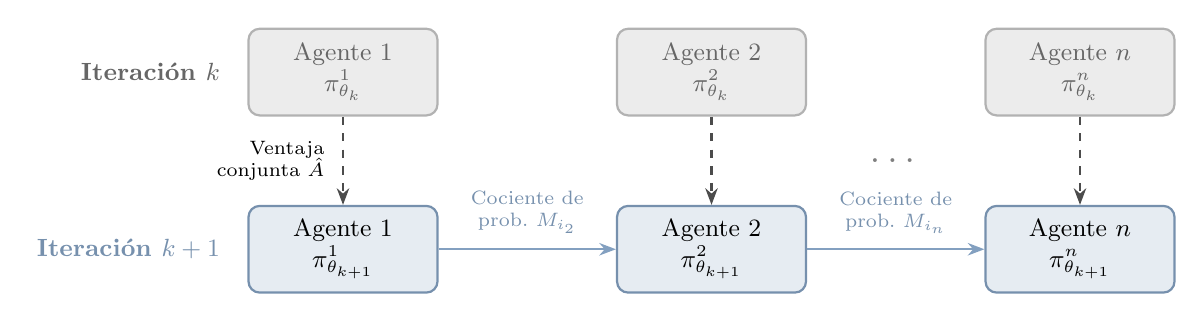
\begin{tikzpicture}[
        scale=0.9,
        >=Stealth,
        box/.style={draw, rounded corners=4pt, thick, align=center, font=\small, fill=white, minimum height=1.1cm, minimum width=2.4cm},
        old/.style={box, draw=gray!60, fill=gray!15, text=gray!80!black},
        new/.style={box, draw=colDatoPrimario!90!black, fill=colDatoPrimario!20},
        arr/.style={-{Stealth[length=6pt]}, thick, draw=black!70},
        lbl/.style={font=\scriptsize, align=right, inner sep=2pt}
    ]
        % Etiquetas de Iteración a la izquierda (ancladas a la derecha con anchor=east para 0% superposición)
        \node[font=\bfseries\small, text=gray!80!black, anchor=east] at (-1.6, 2.5) {Iteración $k$};
        \node[font=\bfseries\small, text=colDatoPrimario!90!black, anchor=east] at (-1.6, 0) {Iteración $k+1$};

        % Nodos de Agentes en Iteración K (Top)
        \node[old] (pi1k) at (0, 2.5) {Agente 1\\$\pi_{\theta_k}^1$};
        \node[old] (pi2k) at (5.2, 2.5) {Agente 2\\$\pi_{\theta_k}^2$};
        \node[old] (pink) at (10.4, 2.5) {Agente $n$\\$\pi_{\theta_k}^n$};

        % Nodos de Agentes en Iteración K+1 (Bottom)
        \node[new] (pi1new) at (0, 0) {Agente 1\\$\pi_{\theta_{k+1}}^1$};
        \node[new] (pi2new) at (5.2, 0) {Agente 2\\$\pi_{\theta_{k+1}}^2$};
        \node[new] (pinnew) at (10.4, 0) {Agente $n$\\$\pi_{\theta_{k+1}}^n$};

        % Actualizaciones verticales (Doble flecha discontinua con texto despejado a la izquierda)
        \draw[arr, dashed] (pi1k) -- node[midway, left=3pt, font=\scriptsize, align=right] {Ventaja\\conjunta $\hat{A}$} (pi1new);
        \draw[arr, dashed] (pi2k) -- (pi2new);
        \draw[arr, dashed] (pink) -- (pinnew);

        % Condicionales secuenciales horizontales (Cociente de probabilidad M)
        \draw[arr, colDatoPrimario, thick] (pi1new.east) -- node[above=2pt, align=center, font=\scriptsize, text=colDatoPrimario!90!black] {Cociente de\\prob. $M_{i_2}$} (pi2new.west);
        \draw[arr, colDatoPrimario, thick] (pi2new.east) -- node[above=2pt, align=center, font=\scriptsize, text=colDatoPrimario!90!black] {Cociente de\\prob. $M_{i_n}$} (pinnew.west);
        
        \node[font=\Large, text=black!50] at (7.8, 1.25) {$\dots$};
    \end{tikzpicture}
    \caption{Esquema de actualización secuencial de HAPPO. A diferencia de PPO Independiente, la actualización de cada agente está matemáticamente condicionada por el cociente de probabilidad compuesto $M_{i_m}$, que propaga los cambios efectuados por los agentes que lo precedieron en la secuencia.}
    \label{fig:happo_sequential}
\end{figure}

\begin{algorithm}[H]
\caption{Algoritmo \textit{Heterogeneous-Agent Proximal Policy Optimization} (HAPPO)}
\label{alg:happo}
\begin{algorithmic}[1]
\State Inicializar los parámetros de las políticas individuales $\{\theta^i, \forall i \in \mathcal{N}\}$ y del crítico centralizado $V_\phi(s)$
\For{iteración $= 1, 2, \dots$}
    \State Recolectar un conjunto de trayectorias $\mathcal{D}$ utilizando la política conjunta $\boldsymbol{\pi}_\theta$
    \State Calcular el estimador de ventaja conjunta $\hat{A}(s, \mathbf{a})$ con GAE a partir del crítico $V_\phi(s)$
    \State Sorteo aleatorio de una permutación de los agentes $i_{1:n} \in \text{Sym}(n)$
    \State Inicializar los factores $M_{i_m}(s, \mathbf{a}) \leftarrow \hat{A}(s, \mathbf{a})$ para todo $m \in \{1, \dots, n\}$
    \For{$m = 1 \dots n$}
        \State Obtener el agente actual $i_m$ y su factor modificador $M_{i_m}(s, \mathbf{a})$
        \State Actualizar $\theta^{i_m}$ a $\theta_{k+1}^{i_m}$ maximizando la pérdida recortada HAPPO:
        \Statex $L^{\text{HAPPO}}(\theta^{i_m}) = \hat{\mathbb{E}}_t \left[ \min\left( r_t^{i_m}(\theta^{i_m}) M_{i_m}(s_t, \mathbf{a}_t), \, \text{clip}\left(r_t^{i_m}(\theta^{i_m}), 1-\epsilon, 1+\epsilon\right) M_{i_m}(s_t, \mathbf{a}_t) \right) \right]$
        \State Recalcular la razón post-optimización: $\rho_{\text{post}}^{i_m} \leftarrow \frac{\pi_{\theta_{k+1}}^{i_m}(a_t^{i_m} \mid o_t^{i_m})}{\pi_{\theta_k}^{i_m}(a_t^{i_m} \mid o_t^{i_m})}$
        \For{$j = m+1 \dots n$}
            \State Actualizar el factor modificador para agentes subsecuentes: 
            \Statex $M_{i_j}(s_t, \mathbf{a}_t) \leftarrow \rho_{\text{post}}^{i_m} \cdot M_{i_j}(s_t, \mathbf{a}_t)$
        \EndFor
    \EndFor
    \State Actualizar el crítico centralizado $\phi$ mediante descenso de gradiente:
    \Statex $\mathcal{L}^{\text{VF}}(\phi) = \hat{\mathbb{E}}_t \left[ \left( V_\phi(s_t) - R_t^{\text{target}} \right)^2 \right]$
\EndFor
\end{algorithmic}
\end{algorithm}

Para finalizar el estudio comparativo de los algoritmos basados en Optimización de Política Próxima en escenarios MARL, la Tabla \ref{tab:marl_ppo_comparison} sintetiza sus principales propiedades operativas, arquitectónicas y teóricas.

\begin{table}[H]
\centering
\caption{Comparación sintética de familias algorítmicas PPO en entornos multi-agente cooperativos.}
\label{tab:marl_ppo_comparison}
\setlength{\tabcolsep}{4pt}
\small
\begin{tabular}{|p{2.6cm}|p{2.8cm}|p{3.1cm}|p{3.2cm}|p{2.8cm}|}
\hline
\textbf{Eje de Análisis} & \textbf{PPO Agente Único} & \textbf{IPPO (Independiente)} & \textbf{MAPPO (CTDE Homogéneo)} & \textbf{HAPPO (HARL Heterogéneo)} \\ \hline
\textbf{Paradigma} & Agente Único & DTE (Descentralizado) & CTDE (Centralizado/Desc.) & CTDE / HARL \\ \hline
\textbf{Arquitectura de Actores} & Único $\pi_\theta(a \mid s)$ & $n$ Actores independientes o compartidos & Compartición de Parámetros ($\pi_\theta$ único) & $n$ Actores heterogéneos ($\pi_{\theta^i}$) \\ \hline
\textbf{Arquitectura del Crítico} & Único $V_\phi(s)$ & $n$ Críticos locales $V_{\phi_i}(o_i)$ & Un Crítico Centralizado $V_\phi(s)$ & Un Crítico Centralizado $V_\phi(s)$ \\ \hline
\textbf{Mecanismo de Optimización} & Simultáneo / Directo & Simultáneo independiente & Simultáneo paralelo & Secuencial con Permutación $i_{1:n}$ \\ \hline
\textbf{Señal de Ventaja} & Ventaja local $\hat{A}(s, a)$ & Ventaja local $\hat{A}_i(o_i, a_i)$ & Ventaja conjunta $\hat{A}(s, \mathbf{a})$ & Factor compuesto $M_{i_{1:m}}(s, \mathbf{a})$ \\ \hline
\textbf{Mejora Monótona} & Garantizada (TRPO/PPO) & Sin garantía (no estacionario) & Sin garantía monótona estricta & Garantizada monótona ($J_{k+1} \ge J_k$) \\ \hline
\textbf{Soporte para Heterogeneidad} & No aplica & Limitado e inestable & Limitado (exige Parameter Sharing) & Nativo y matemáticamente exacto \\ \hline
\end{tabular}
\end{table}

\section{Control de Tráfico Urbano mediante MARL}

Una vez establecidos los marcos teóricos de la Ingeniería de Tránsito y del Aprendizaje por Refuerzo Multi-Agente, esta sección formaliza el mapeo directo entre los conceptos físicos del dominio del tráfico y la tupla de decisión secuencial Dec-POMDP, definiendo la arquitectura de interacción entre el simulador y los controladores inteligentes.

\subsection{Formalización del Control Semafórico Coordinado como Dec-POMDP}

En el contexto del control adaptativo de red, cada intersección semaforizada se modela como un agente inteligente $i \in \mathcal{N} = \{1, \dots, n\}$. La interacción entre la red vial simulada en SUMO y el sistema de control se formaliza mediante los elementos de la tupla Dec-POMDP:

\begin{itemize}
    \item \textbf{Entorno ($environment$) e Interfaz TraCI:} El simulador microscópico SUMO actúa como el entorno dinámico. A través de la interfaz TraCI (\textit{Traffic Control Interface}) y la librería de abstracción SUMO-RL \cite{AlegreLSUMORLDoc}, se establece un bucle de control discreto paso a paso donde el sistema lee la telemetría del tráfico y envía comandos de fase a los semáforos.
    \item \textbf{Espacio de observaciones ($o_i \in \Omega_i$):} Vector de características locales registrado en los accesos de la intersección $i$ en el instante $t$. Incluye la longitud de cola por carril ($q_l$), la densidad u ocupación ($k_l$), la velocidad media espacial ($v_l$), el número de vehículos detenidos y el indicador de la fase semafórica activa actualmente.
    \item \textbf{Espacio de acciones ($a_i \in \mathcal{A}_i$):} Selección discreta de la siguiente fase semafórica a activar o mantener. Cada decisión se ejecuta durante un tiempo de verde fijo $g$ (e.g., 5 segundos). Si el agente decide cambiar de fase, el entorno intercala de forma automática los intervalos de seguridad física ($t_{\text{amarillo}} + t_{\text{rojo\_todo}}$) antes de iniciar la nueva fase.
    \item \textbf{Función de recompensa ($R_i$):} En el marco abstracto del Dec-POMDP, la recompensa actúa como una señal escalar de realimentación diseñada para incentivar la fluidez vehicular penalizando las manifestaciones físicas de la congestión (colas, demoras y detenciones). La especificación matemática exacta y las distintas funciones de recompensa evaluadas y comparadas en este trabajo se formulan formalmente en el Capítulo \ref{capitulo:metodologia} (Metodología).
    \item \textbf{Coordinación y prevención de congestión (\textit{Spillback}):} Las decisiones operativas de un semáforo afectan de forma directa a las intersecciones adyacentes. Una fase verde prolongada en un acceso principal descarga un pelotón de vehículos que avanza hacia el nodo contiguo; si ese nodo no ajusta oportunamente su temporización, la cola resultante puede bloquear la intersección aguas arriba (\textit{spillback}). Mediante algoritmos CTDE (MAPPO) y HARL (HAPPO), los agentes aprenden a coordinar secuencias de verde continuas (olas verdes adaptativas), maximizando la capacidad de descarga global.
\end{itemize}

\subsection{Funciones de Recompensa en Control Semafórico}

En la formalización de un Dec-POMDP para el control semafórico adaptativo, la función de recompensa $R_i$ constituye la señal de realimentación cuantitativa mediante la cual el sistema guía el aprendizaje de los agentes \cite{MDPI_Infrastructures2025_RLReview}. En este trabajo, el marco computacional \texttt{marlTLC} formaliza e implementa un conjunto jerárquico de funciones de recompensa orientadas a resolver el compromiso entre la optimización local y la coordinación sistémica:

\begin{itemize}
    \item \textbf{Formulaciones Diferenciales y Absolutas:} Las recompensas absolutas, como la demora negativa ($R = -W_{\text{acc}}$) o la longitud de cola negativa ($R = -N_{\text{queue}}$), penalizan permanentemente el estado actual del tráfico. Sin embargo, en simulación microscópica con flujos dinámicos, esta penalización absoluta acumula deriva de varianza a lo largo del episodio. Las formulaciones diferenciales computan la mejora discreta respecto al paso temporal anterior:
    \begin{equation}
        R_{\text{diff\_halted}} = N_{\text{halted}}(t-1) - N_{\text{halted}}(t)
    \end{equation}
    \begin{equation}
        R_{\text{diff\_waiting}} = W_{\text{acc}}(t-1) - W_{\text{acc}}(t)
    \end{equation}
    donde un valor positivo indica una reducción efectiva en el número de vehículos detenidos o en la demora acumulada, proporcionando un gradiente de progreso local paso a paso que estabiliza la asignación de crédito temporal \cite{difference_rewards}.
    \item \textbf{Presión de Tráfico (\textit{PressureReward}):} Basada en la teoría de flujo de saturación y control de presión máxima (\textit{Max-Pressure}) \cite{presslight2019}, la presión $P_i$ en una intersección $i$ evalúa la diferencia entre los vehículos detenidos en los carriles entrantes ($L_{\text{in}}$) y los vehículos en los carriles salientes ($L_{\text{out}}$):
    \begin{equation}
        P_i = \left| \sum_{l \in L_{\text{in}}} N_{\text{halted}, l} - \sum_{m \in L_{\text{out}}} N_{\text{halted}, m} \right|
    \end{equation}
    Definiendo $R_{\text{pressure}} = -P_i$, la maximización del incentivo equivale a igualar las tasas de descarga y prevenir la acumulación de presión aguas abajo.
    \item \textbf{Normalización por Volumen Vehicular:} Para evitar que intersecciones con mayor volumen dominen desproporcionadamente la señal de aprendizaje en redes heterogéneas, se aplica la normalización por la cantidad de vehículos activos:
    \begin{equation}
        R_{\text{diff\_waiting\_norm}} = \frac{W_{\text{acc}}(t-1) - W_{\text{acc}}(t)}{\max(N_{\text{veh}}(t), 1)}
    \end{equation}
    \item \textbf{Mezcla Cooperativa Vecinal ($\lambda$-mix):} Para mitigar el comportamiento egoísta o miope de agentes independientes, la función \texttt{NeighborMixReward} combina de manera convexa la señal local $L_i$ con la media de las recompensas observadas en las intersecciones vecinas $N_i$:
    \begin{equation}
        R_i = (1 - \lambda) L_i + \lambda \left( \frac{1}{|\text{Nei}(i)|} \sum_{j \in \text{Nei}(i)} L_j \right)
    \end{equation}
    donde $\lambda = \frac{w}{1+w} \in [0, 1)$ parametriza la fracción de cooperación vecinal (siendo $w \ge 0$ el peso de mezcla histórica). Esta señal compartida promueve la coordinación espacial y favorece la aparición espontánea de olas verdes entre nodos adyacentes.
    \item \textbf{Penalización por Desbordamiento de Cola (\textit{Spillback Penalty}):} Cuando la densidad en los carriles salientes supera el umbral crítico de capacidad ($k \ge 95\%$), la señal \texttt{SpillbackPenaltyReward} inyecta un castigo escalar severo. Esto desincentiva acciones que saturen los accesos contiguos, bloqueando físicamente el cruce aguas arriba (\textit{spillback}).
\end{itemize}

\section{Frameworks Tecnológicos de Escalado y Optimización}

La evaluación experimental de algoritmos de Aprendizaje por Refuerzo Multi-Agente Profundo en escenarios de simulación microscópica exige infraestructuras de cómputo capaces de escalar la recolección de experiencia y optimizar iterativamente espacios de hiperparámetros de alta dimensionalidad.

\subsection{Ecosistema Ray: Ray Core, Ray Tune y RLlib}

Ray es un framework de computación distribuida de código abierto diseñado para escalar aplicaciones de inteligencia artificial y aprendizaje por refuerzo \cite{ray_doc_2025}. En esta investigación, la pila tecnológica se apoya en tres módulos fundamentales del ecosistema Ray:

\begin{itemize}
    \item \textbf{Ray Core:} Infraestructura distribuida subyacente basada en el modelo de actores y tareas asíncronas. Permite gestionar de manera paralela múltiples procesos de simulación en SUMO interactuando a través de TraCI en entornos multinúcleo o distribuidores de cómputo HPC \cite{ray_doc_2025}.
    \item \textbf{Ray Tune:} Plataforma distribuida para la selección de modelos y optimización de hiperparámetros \cite{liaw2018tune}. Ray Tune coordina la ejecución paralela de pruebas (\textit{trials}), gestiona dinámicamente los recursos de hardware (CPU/GPU) por experimento y registra métricas de telemetría en tiempo real.
    \item \textbf{RLlib:} Librería de referencia para aprendizaje por refuerzo distribuido masivo \cite{liang2018rllib}. Ofrece abstracciones nativas para entornos multi-agente bajo el paradigma CTDE (MAPPO y HAPPO), soportando compartición de parámetros (\textit{Parameter Sharing}), vectorización paralela de entornos TraCI y recolección eficiente de trayectorias \textit{on-policy}.
\end{itemize}

\subsection{Framework Optuna y Pipeline de Optimización Multietapa}

Para sintonizar de forma rigurosa los hiperparámetros algorítmicos (como la tasa de aprendizaje $\alpha$, el rango de recorte PPO $\epsilon$, el número de épocas $K$ y la entropía), se emplea el framework de optimización automática Optuna \cite{akiba2019optuna, optuna_doc_2025}.

\subsubsection{Optimización Bayesiana TPE y Poda Asíncrona ASHA}

La exploración estocástica del espacio de búsqueda en Optuna se estructura mediante dos componentes algorítmicos principales:
\begin{itemize}
    \item \textbf{Muestreo Bayesiano TPE (\textit{Tree-structured Parzen Estimator}):} A diferencia de la búsqueda aleatoria o en grilla, TPE construye estimadores de densidad condicional no paramétricos $l(x)$ y $g(x)$ para modelar las distribuciones de hiperparámetros asociadas a los desempeños superiores e inferiores observados, respectivamente \cite{akiba2019optuna}. El algoritmo muestrea iterativamente las regiones que maximizan la razón de verosimilitud (\textit{Likelihood Ratio}), concentrando la exploración en las cuencas de convergencia más prometedoras.
    \item \textbf{Poda Asíncrona ASHA (\textit{Asynchronous Successive Halving Algorithm}):} Dado el costo computacional de ejecutar simulaciones completas en SUMO, ASHA monitorea asíncronamente las curvas de aprendizaje intermedias y cancela tempranamente (\textit{pruning}) las pruebas que se ubican en los percentiles inferiores de desempeño \cite{li2020system}. Se define un período de gracia (\textit{grace period}) adecuado para preservar pruebas MARL cuya convergencia coordinada suele ser lenta en las fases iniciales.
\end{itemize}

\subsubsection{Pipeline Multietapa y Métrica de Retorno Robusto al Riesgo (CVaR)}

Con el propósito de mitigar la maldición de la dimensionalidad sin introducir sesgo humano temprano, la optimización se organiza en un \textbf{Pipeline Multietapa}:
\begin{enumerate}
    \item \textbf{Fase 1 (Exploración Estocástica de Amplio Espectro - \textit{Broad Search}):} Explora el espacio global mediante distribuciones no restringidas en Optuna (\texttt{loguniform}, \texttt{uniform} extensos), identificando las cuencas de atracción del algoritmo en distintos escenarios viales.
    \item \textbf{Fase 2 (Refinamiento Bayesiano Guiado por Evidencia - \textit{Refined Search}):} Bajo el principio de la \textbf{Navaja de Ockham Bayesiana}, refina las distribuciones probabilísticas alrededor de los valles óptimos de la Fase 1. Si un parámetro convergió contra el límite del rango inicial (censura de frontera), el método expande formalmente sus fronteras para verificar la existencia del óptimo global.
\end{enumerate}

En entornos MARL, los algoritmos sufren con frecuencia de \textbf{colapso de política} (\textit{Policy Collapse}), una degradación repentina de las políticas cooperativas causada por la alta varianza del aprendizaje concurrente \cite{yu2022surprising}. Para forzar a Optuna a seleccionar únicamente configuraciones estables y seguras, la función objetivo abandona el promedio aritmético simple en favor de una métrica de \textbf{Retorno Robusto al Riesgo} inspirada en el Valor en Riesgo Condicional (CVaR):
\begin{equation}
    \text{Robust\_Return} = \mathbb{E}[\mathcal{R}] - \alpha \cdot \left( \mathbb{E}[\mathcal{R}] - \min(\mathcal{R}) \right)
\end{equation}
donde $\mathbb{E}[\mathcal{R}]$ representa la recompensa promedio esperada del lote, $\min(\mathcal{R})$ es la peor recompensa episódica registrada en el lote, y $\alpha \in [0, 1]$ es el factor de aversión al riesgo (típicamente $\alpha = 0.5$). Penalizar la varianza inferior descarta configuraciones inestables y garantiza la mejora monótona del desempeño conjunto en el sistema de control.

\chapter{Metodología y Diseño Experimental}
\label{capitulo:metodologia}

Este capítulo describe el diseño experimental, la operacionalización de las variables, la construcción de los escenarios de simulación y la arquitectura computacional utilizada. También presenta los protocolos de entrenamiento y evaluación empleados para comparar \acrshort{acr-mappo} y \acrshort{acr-happo} con las líneas de base \acrshort{acr-ippo} e \acrshort{acr-idqn}. El estudio adopta un enfoque cuantitativo y un diseño comparativo con replicaciones independientes y comparaciones pareadas por semilla: cada ejecución de entrenamiento produce una política y cada política se evalúa bajo semillas y condiciones de demanda previamente definidas. La simulación microscópica del tránsito funciona como un entorno controlado; el escenario de la Ciudad de Mendoza se interpreta como una construcción sintética restringida por datos parciales, no como un gemelo digital completo.

\section{Enfoque y Diseño de Investigación}
\label{sec:enfoque_diseno}

Este trabajo adopta un \textbf{diseño experimental cuantitativo comparativo con replicaciones independientes y comparaciones pareadas por semilla}. Los factores principales son la familia algorítmica, la arquitectura de la red neuronal, el grado de cooperación vecinal $\rho_{\mathrm{coop}}$ y el escenario de tránsito. Las políticas se comparan dentro de cada escenario y, de forma complementaria, se estudia cómo cambia su comportamiento al aumentar la escala o modificar la topología. Dado que también cambian la demanda y el número de agentes, las comparaciones entre escenarios se expresan mediante métricas absolutas y mediante variaciones relativas respecto del controlador de tiempo fijo del mismo escenario.

La simulación microscópica se utiliza como plataforma experimental por tres razones. El simulador utilizado es \acrshort{acr-sumo} \cite{SUMO2026_SUMO}:
\begin{enumerate}
    \item \textbf{Seguridad y viabilidad operacional:} evaluar algoritmos estocásticos de aprendizaje en tiempo real sobre una red urbana real implicaría riesgos para la seguridad vial y la fluidez del tránsito.
    \item \textbf{Aislamiento de variables exógenas:} la simulación permite controlar perturbaciones que no forman parte del modelo, como condiciones meteorológicas, siniestros viales o fluctuaciones externas.
    \item \textbf{Replicabilidad:} la fijación de semillas pseudoaleatorias permite someter los distintos controladores a las mismas condiciones de demanda.
\end{enumerate}

Para evaluar las políticas se emplean métricas físicas extraídas de la telemetría microscópica de \acrshort{acr-sumo}, principalmente del archivo \texttt{TripInfo}. La métrica primaria de la búsqueda de hiperparámetros es la espera media por vehículo insertado; las demás métricas se utilizan para interpretar eficiencia, atención de la demanda, equidad y estabilidad:
\begin{itemize}
    \item \textbf{Espera media de los vehículos insertados ($\bar{w}_{\mathrm{ins}}$):} métrica operacional obtenida de \texttt{TripInfo}:
    \begin{equation}
        \bar{w}_{\mathrm{ins}} = \frac{\sum_{v\in\mathcal{V}_{\mathrm{ins}}} w_v}{|\mathcal{V}_{\mathrm{ins}}|},
        \qquad w_v=\texttt{waitingTime}_v .
        \label{eq:espera_media_insertados}
    \end{equation}
    En la ecuación \eqref{eq:espera_media_insertados}, $\mathcal{V}_{\mathrm{ins}}$ es el conjunto de vehículos insertados en la ventana, $w_v$ es el tiempo de espera del vehículo $v$ en segundos y $|\mathcal{V}_{\mathrm{ins}}|$ es su cardinalidad. SUMO define \texttt{waitingTime} como el tiempo con velocidad menor o igual a $0,1\,\mathrm{m/s}$; por tanto, la métrica es un promedio en segundos por vehículo y no una suma en vehículo$\cdot$segundo. El entorno conserva además la espera integrada de los vehículos expuestos durante la ventana, pero esta magnitud no constituye el objetivo principal.
    \item \textbf{\gls{acr-cr}:} proporción de la demanda cargada que completa su itinerario dentro del horizonte de evaluación. La métrica también contabiliza los vehículos retenidos en los accesos de origen por sobresaturación:
    \begin{equation}
        \text{CR} = \frac{\text{throughput}}{\text{departed} + \text{pending\_vehicles\_end}}
        \label{eq:tasa_completitud}
    \end{equation}
    La ecuación \eqref{eq:tasa_completitud} relaciona los vehículos completados con la demanda que ingresó o quedó retenida. Todos sus términos son conteos del mismo horizonte: $\text{throughput}$ corresponde a los vehículos que completaron su itinerario, $\text{departed}$ a los que ingresaron a la calzada y $\text{pending\_vehicles\_end}$ a los que permanecieron en origen sin poder insertarse al cierre de la ventana. Cuando el simulador no descarta vehículos, se cumple la conservación $\text{loaded} \approx \text{departed} + \text{pending\_vehicles\_end}$ y el denominador de CR coincide con la carga de la ventana \cite{SUMO2026_SUMO}. También se registran la \gls{acr-ir} ($\text{IR} = \frac{\text{inserted}}{\text{loaded}}$) y la \gls{acr-ci} ($\text{CI} = \frac{\text{arrived\_inserted}}{\text{inserted}}$). Esta última tasa se restringe a los vehículos insertados durante la ventana que también completan su itinerario en ella; evita mezclar en el numerador vehículos presentes desde el calentamiento. Las tres tasas se informan conjuntamente con la métrica primaria porque un promedio calculado sobre los vehículos que circulan puede mejorar si un controlador restringe la inserción de demanda sin aliviar la congestión, efecto documentado en la evaluación de control semafórico por aprendizaje por refuerzo \cite{jiang2024xlight}.
    \item \textbf{Equidad espacial de demoras (coeficiente de Gini, $G_{\text{wait}}$):} cuantifica la desigualdad en la distribución del tiempo de espera medio entre las intersecciones semaforizadas de la red:
    \begin{equation}
        G_{\text{wait}} = \frac{2 \sum_{i=1}^{N} i \cdot \bar{w}_{(i)} - (N + 1) \sum_{i=1}^{N} \bar{w}_{(i)}}{N \sum_{i=1}^{N} \bar{w}_{(i)}}
        \label{eq:gini_espera}
    \end{equation}
    La ecuación \eqref{eq:gini_espera} se calcula después de ordenar los tiempos de espera medios. En ella, $\bar{w}_{(1)} \le \bar{w}_{(2)} \le \dots \le \bar{w}_{(N)}$ son los tiempos de espera medios ordenados de cada intersección y $N$ es el total de intersecciones semaforizadas. Cada $\bar{w}_i$ es el promedio temporal, sobre los pasos de decisión de la ventana controlada, de la espera media de los vehículos presentes en los carriles controlados por esa intersección. Las intersecciones entran con peso uniforme, sin ponderar por demanda: el índice describe la distribución interseccional del servicio, no la distribución entre vehículos individuales. Esta métrica se complementa con la desviación estándar inter-intersección ($\sigma_{\text{wait}}$) para evaluar si las políticas aprendidas distribuyen equitativamente el servicio o si sacrifican accesos secundarios en favor de arterias dominantes.
    \item \textbf{Pérdida temporal ($\overline{\ell}$):} promedio de \texttt{timeLoss} por vehículo insertado, que cuantifica el tiempo perdido respecto de la velocidad ideal del vehículo. Se registra como métrica secundaria porque incluye desaceleraciones y conflictos de circulación que no siempre se reflejan en la espera.
\end{itemize}

El archivo \texttt{TripInfo} solo incluye viajes finalizados cuando se escribe durante la ejecución; por eso el entorno activa \texttt{--tripinfo-output.write-unfinished} y cierra la conexión al terminar el episodio. Las métricas se calculan entonces sobre todos los registros válidos cuyo atributo de partida pertenece a la ventana, incluidos los viajes que aún no llegaron a destino. La documentación de SUMO define de forma independiente \texttt{waitingTime} y \texttt{timeLoss}; no se los intercambia en el análisis.

La figura \ref{fig:flujo_metodologico_general} resume las siete etapas de la investigación. En este contexto, \emph{etapa} designa una parte del procedimiento metodológico y no una fase del ciclo semafórico.

\begin{figure}[H]
\centering
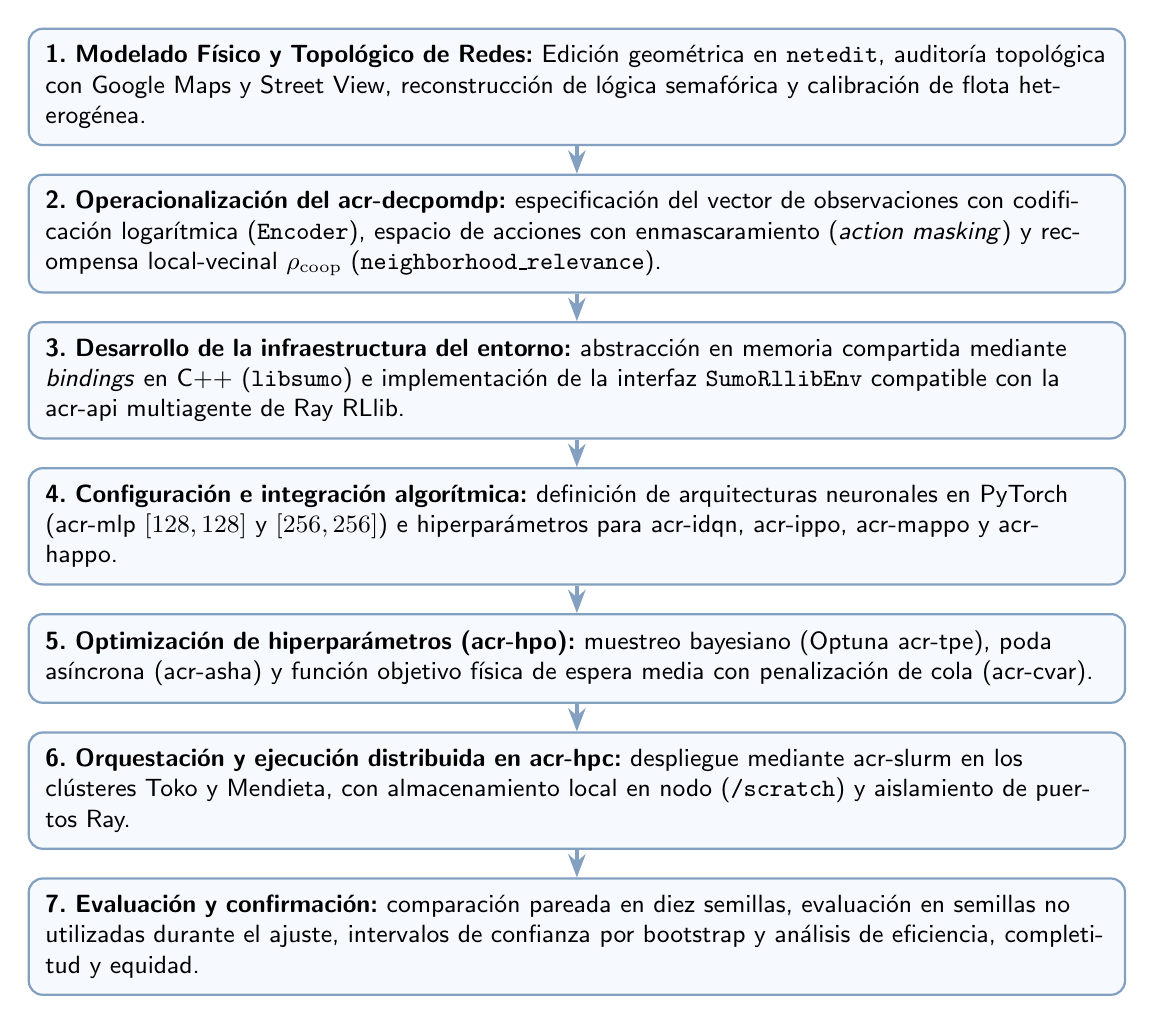
\begin{tikzpicture}[
  node distance=0.35cm and 0cm,
  font=\sffamily\small,
  >=Stealth,
  paso/.style={rectangle, draw=colEntorno!80!black, fill=colEntorno!10, rounded corners=5pt, thick, text width=13.5cm, align=left, inner sep=6pt}
]
  \node[paso] (p1) {\textbf{1. Modelado Físico y Topológico de Redes:} Edición geométrica en \texttt{netedit}, auditoría topológica con Google Maps y Street View, reconstrucción de lógica semafórica y calibración de flota heterogénea.};
  \node[paso, below=of p1] (p2) {\textbf{2. Operacionalización del \acrshort{acr-decpomdp}:} especificación del vector de observaciones con codificación logarítmica (\texttt{Encoder}), espacio de acciones con enmascaramiento (\textit{action masking}) y recompensa local-vecinal $\rho_{\mathrm{coop}}$ (\texttt{neighborhood\_relevance}).};
  \node[paso, below=of p2] (p3) {\textbf{3. Desarrollo de la infraestructura del entorno:} abstracción en memoria compartida mediante \textit{bindings} en C++ (\texttt{libsumo}) e implementación de la interfaz \texttt{SumoRllibEnv} compatible con la \gls{acr-api} multiagente de Ray RLlib.};
  \node[paso, below=of p3] (p4) {\textbf{4. Configuración e integración algorítmica:} definición de arquitecturas neuronales en PyTorch (\gls{acr-mlp} $[128, 128]$ y $[256, 256]$) e hiperparámetros para \acrshort{acr-idqn}, \acrshort{acr-ippo}, \acrshort{acr-mappo} y \acrshort{acr-happo}.};
  \node[paso, below=of p4] (p5) {\textbf{5. Optimización de hiperparámetros (\acrshort{acr-hpo}):} muestreo bayesiano (Optuna \gls{acr-tpe}), poda asíncrona (\gls{acr-asha}) y función objetivo física de espera media con penalización de cola (\gls{acr-cvar}).};
  \node[paso, below=of p5] (p6) {\textbf{6. Orquestación y ejecución distribuida en \gls{acr-hpc}:} despliegue mediante \gls{acr-slurm} en los clústeres Toko y Mendieta, con almacenamiento local en nodo (\texttt{/scratch}) y aislamiento de puertos Ray.};
  \node[paso, below=of p6] (p7) {\textbf{7. Evaluación y confirmación:} comparación pareada en diez semillas, evaluación en semillas no utilizadas durante el ajuste, intervalos de confianza por bootstrap y análisis de eficiencia, completitud y equidad.};

  \draw[->, line width=1.2pt, colEntorno!80!black] (p1) -- (p2);
  \draw[->, line width=1.2pt, colEntorno!80!black] (p2) -- (p3);
  \draw[->, line width=1.2pt, colEntorno!80!black] (p3) -- (p4);
  \draw[->, line width=1.2pt, colEntorno!80!black] (p4) -- (p5);
  \draw[->, line width=1.2pt, colEntorno!80!black] (p5) -- (p6);
  \draw[->, line width=1.2pt, colEntorno!80!black] (p6) -- (p7);
\end{tikzpicture}
\caption{Flujo metodológico de la investigación experimental. Los siete recuadros representan, de arriba hacia abajo, las etapas de modelado de redes, formulación del problema, desarrollo del entorno, integración algorítmica, optimización de hiperparámetros, ejecución distribuida y evaluación estadística; las flechas indican la dependencia secuencial entre ellas.}
\label{fig:flujo_metodologico_general}
\end{figure}

La figura \ref{fig:flujo_metodologico_general} comienza con la construcción física y topológica de las redes que sirven como escenarios experimentales. Sobre esos escenarios se define el problema de decisión: qué observa cada agente, qué acciones puede ejecutar y qué recompensa recibe. La tercera etapa implementa esas definiciones en el entorno de simulación, y la cuarta incorpora los algoritmos y sus redes neuronales. Una vez que el sistema puede entrenarse, la quinta etapa busca configuraciones de hiperparámetros. La sexta distribuye las ejecuciones en la infraestructura de cómputo, y la séptima compara las políticas mediante métricas físicas y análisis de variabilidad. Las flechas verticales expresan la dependencia metodológica y no representan ejecución simultánea.

\section{Especificación del Ecosistema Tecnológico}
\label{sec:stack_tecnologico}

Para garantizar la reproducibilidad científica, la tabla \ref{tab:stack_tecnologico} detalla las librerías, marcos de trabajo y plataformas de cómputo sobre las cuales se desarrolló y ejecutó el entorno \texttt{marlTLC}. En esta sección, la \gls{telemetria} es el conjunto de mediciones que el simulador registra durante la ejecución; un \gls{framework} proporciona interfaces y componentes reutilizables para construir el sistema; un \gls{binding} conecta una biblioteca escrita en un lenguaje con otro, y la \gls{serializacion} convierte un objeto o mensaje en una representación que puede almacenarse o transmitirse. Los procesos denominados \textit{env runners} generan trayectorias al interactuar con el entorno y los \textit{learners} actualizan los parámetros de las redes a partir de esas trayectorias. Estas definiciones permiten interpretar la tabla sin suponer familiaridad previa con la infraestructura de software.

\begin{table}[H]
\centering
\caption{Especificación de las tecnologías y herramientas utilizadas en la investigación.}
\label{tab:stack_tecnologico}
\setlength{\tabcolsep}{5pt}
\small
\begin{tabular}{|>{\raggedright\arraybackslash}p{3.5cm}|>{\raggedright\arraybackslash}p{3.5cm}|>{\raggedright\arraybackslash}p{6.2cm}|}
\hline
\textbf{Componente} & \textbf{Herramienta / Versión} & \textbf{Función Metodológica} \\ \hline
Lenguaje de Programación & Python 3.10+ & Núcleo del sistema, tipado estático (\texttt{typing.Protocol}) y scripts de orquestación. \\ \hline
Simulador de Tránsito & \acrshort{acr-sumo} 1.20+ / \acrshort{acr-traci} & Simulación microscópica, dinámica cinemática y telemetría de red. \\ \hline
\textit{Bindings} de Simulación & \texttt{libsumo} (C++) & Ejecución de la simulación en memoria compartida mediante \textit{bindings} en C++ (\texttt{LIBSUMO\_AS\_TRACI=1}). \\ \hline
Marco de trabajo \acrshort{acr-marl} (\textit{framework}) & Ray RLlib 2.x \cite{liang2018rllib} & Abstracción de entornos multiagente (\texttt{MultiAgentEnv}, \texttt{RLModuleSpec}, \texttt{LearnerGroup}). \\ \hline
Aprendizaje Profundo & PyTorch 2.x & Modelado neuronal y optimización (Actor-Crítico \acrshort{acr-mlp}, \textit{action masking}). \\ \hline
Optimización Automática & Optuna 3.x \cite{akiba2019optuna} & Muestreo Bayesiano \acrshort{acr-tpe} y poda asíncrona de pruebas (\acrshort{acr-asha} \cite{li2020system}). \\ \hline
Infraestructura \acrshort{acr-hpc} & Clústeres Toko y Mendieta & Cómputo distribuido multinúcleo gestionado vía \acrshort{acr-slurm} con \gls{acr-es} local (\texttt{/scratch}). \\ \hline
\end{tabular}
\end{table}

Estas capas se integran de la siguiente manera. Python coordina la ejecución y Ray RLlib gestiona los procesos concurrentes de recolección de trayectorias (\textit{env runners}). PyTorch calcula las derivadas y optimiza las redes neuronales en los módulos de aprendizaje (\textit{learners}). \texttt{SumoRllibEnv} encapsula la lógica episódica y \texttt{libsumo} ejecuta los cálculos de cinemática vehicular en la memoria del proceso, sin comunicación por red ni serialización \gls{acr-tcp}.

\section[Diseño y Calibración de Escenarios de Tránsito en SUMO]{Diseño y Calibración de Escenarios de Tránsito en \acrshort{acr-sumo}}
\label{sec:diseno_escenarios}

La evaluación empírica se realiza sobre cuatro escenarios de red en \acrshort{acr-sumo}. Las redes se construyen con la herramienta gráfica \texttt{netedit}, los utilitarios de conversión \texttt{netconvert} y scripts de generación en Python. En conjunto, los escenarios representan distintas complejidades topológicas y condiciones de flujo.

\subsection{Modelado Geométrico y Sanitización Topológica}
\label{subsec:metodologia_modelado_sumo}

La construcción de las redes de simulación sigue un procedimiento de diseño y validación en \acrshort{acr-sumo}:
\begin{enumerate}
    \item \textbf{Diseño geométrico y accesos:} definición de calzadas, cantidad de carriles por aproximación y longitudes de almacenamiento en \texttt{netedit} o a partir de datos cartográficos de \acrshort{acr-osm}.
    \item \textbf{Auditoría y corrección topológica:} verificación de los sentidos de circulación, la cantidad de carriles, las conexiones de giro y las maniobras prohibidas. La revisión se contrasta con imágenes satelitales y vistas de calle de Google Maps y Google Street View.
    \item \textbf{Configuración semafórica:} las configuraciones de los semáforos estáticos corresponden a los planes generados por defecto por \acrshort{acr-sumo} (\texttt{netconvert --tls.rebuild}) al compilar la red. Los programas de fases y los tiempos de ciclo originales se mantienen sin cambios. La correspondencia entre los enlaces físicos y los índices de control semafórico (\textit{linkIndex}) se recalcula para conservar la consistencia topológica.
\end{enumerate}

\subsection{Escenarios Sintéticos: \texorpdfstring{$3\times1$, $3\times3$ y $4\times4\_H$}{3x1, 3x3 y 4x4-H}}
\label{subsec:escenarios_sinteticos}

Todas las redes sintéticas comparten las siguientes reglas operacionales:
\begin{itemize}
    \item \textbf{Límite de velocidad:} $13.89\text{ m/s}$ ($50\text{ km/h}$) en todas las arterias urbanas.
    \item \textbf{Flota vehicular heterogénea:} se definieron tres perfiles cinemáticos en el archivo \texttt{urban\_vehicle\_mix.add.xml}, a partir de los modelos disponibles en el simulador \cite{SUMO2026_SUMO}:
    \begin{enumerate}
        \item \texttt{SLOWVEHTYPE} ($25\%$): perfil de menor aceleración y velocidad máxima ($a = 1.9\text{ m/s}^2, d = 4.0\text{ m/s}^2, v_{\max} = 8.33\text{ m/s} = 30\text{ km/h}$).
        \item \texttt{MEDVEHTYPE} ($60\%$): perfil de referencia. Parámetros: $a = 2.6\text{ m/s}^2$ y $d = 4.5\text{ m/s}^2$; $v_{\max} = 13.89\text{ m/s} = 50\text{ km/h}$.
        \item \texttt{FASTVEHTYPE} ($15\%$): perfil de mayor aceleración, $a = 3.1\text{ m/s}^2$ y $d = 5.0\text{ m/s}^2$; $v_{\max} = 19.44\text{ m/s} = 70\text{ km/h}$.
    \end{enumerate}
    Parámetros compartidos: longitud $4.5\text{ m}$, brecha mínima de seguridad (\textit{minGap}) $2.5\text{ m}$ e imperfección del conductor de Krauss $\sigma = 0.5$.
    \item \textbf{Generación de demanda por zonas (\acrshort{acr-taz}):} las rutas se generan mediante \texttt{random\_routes\_taz.py} a partir de matrices de zonas de asignación de tránsito. Los tres escenarios sintéticos almacenan flujos con el atributo \texttt{vehsPerHour}; la demanda nominal se expresa en vehículos por hora y SUMO inserta los vehículos conforme al flujo solicitado. No se atribuye a estas redes un proceso de llegadas exponencial.
    \item \textbf{Calibración por bisección:} los flujos totales de los tres escenarios sintéticos se ajustaron mediante bisección bajo control semafórico de tiempo fijo, con el objetivo de obtener una tasa de completitud sobre los vehículos insertados (\acrshort{acr-ci}) próxima a $0,70$. El horizonte de referencia fue de $4200\text{ s}$, compuesto por $600\text{ s}$ de calentamiento y $3600\text{ s}$ de control.
\end{itemize}

La Tabla \ref{tab:escenarios_sinteticos} resume las características verificadas y los flujos nominales obtenidos para los tres escenarios sintéticos.

\begin{table}[H]
\centering
\caption{Características verificadas de los escenarios sintéticos.}
\label{tab:escenarios_sinteticos}
\small
\begin{tabular}{lrrrr}
\hline
\textbf{Escenario} & \textbf{Agentes} & \textbf{Tramos} & \textbf{Carriles} & \textbf{Flujo nominal (veh/h)} \\
\hline
$3\times1$ & 3 & 20 & 40 & 3.260 \\
$3\times3$ & 9 & 48 & 96 & 7.087 \\
$4\times4\_H$ & 16 & 71 & 166 & 7.202 \\
\hline
\end{tabular}
\end{table}

Los flujos finales de $3.260$ veh/h para $3\times1$, $7.087$ veh/h para $3\times3$ y $7.202$ veh/h para $4\times4_H$ fueron los obtenidos con esa calibración. El objetivo de completitud cercano a $0,70$ fija condiciones de congestión comparables para el estudio sintético; no establece una equivalencia exacta de demanda entre topologías ni valida una demanda urbana.

Las tres topologías sintéticas cumplen funciones analíticas complementarias:
\begin{itemize}
    \item \textbf{Corredor arterial $3\times1$ (3.260 veh/h):} tres intersecciones dispuestas en línea. El perfil canónico asigna explícitamente $40\%$ al par $3\to4$ y $35\%$ al par $4\to3$; el remanente se distribuye de forma reproducible entre los pares válidos restantes. Su disposición permite estudiar la propagación longitudinal de colas y la coordinación de fases sobre las corrientes predominantes.
    \item \textbf{Malla simétrica $3\times3$ (7.087 veh/h):} nueve intersecciones organizadas en una cuadrícula cerrada. El perfil canónico asigna $20\%$, $17,5\%$, $17,5\%$ y $20\%$ a los pares $5\to6$, $6\to5$, $10\to1$ y $1\to10$, respectivamente; el $25\%$ restante se asigna entre los pares válidos. La interconexión permite estudiar el desbordamiento de colas (\textit{spillback}) y la estabilidad de \acrshort{acr-marl} bajo congestión severa.
    \item \textbf{Cuadrícula $4\times4\_H$ (7.202 veh/h):} dieciséis intersecciones con geometría heterogénea. El perfil canónico asigna $20\%$, $17,5\%$, $17,5\%$ y $20\%$ a los pares $5\to9$, $6\to5$, $13\to1$ y $1\to13$, respectivamente; el $25\%$ restante se distribuye entre los pares válidos.
\end{itemize}

\subsection{Escenario urbano de la Ciudad de Mendoza}
\label{subsec:escenario_mendoza}

Para estudiar el comportamiento de los controladores en una red urbana de mayor escala, se construyó un escenario del microcentro de la Ciudad de Mendoza a partir de su infraestructura topológica y de una serie temporal parcial de aforo vehicular captada mediante una cámara termográfica. La red representa la geometría urbana, pero su demanda completa se aproxima mediante supuestos espaciales y un volumen nominal; por eso el escenario no se presenta como una validación del tránsito total de la ciudad. El diseño experimental prevé un ajuste de hiperparámetros, entrenamiento y evaluación propios para cada uno de los cuatro algoritmos en este escenario; no se transfieren pesos ni configuraciones finales desde las redes sintéticas.

\subsubsection{Posición Metodológica: Escenario Restringido por Datos}
\label{subsubsec:mendoza_posicion_metodologica}

El escenario de Mendoza se considera un \textbf{escenario sintético restringido por datos} (\textit{data-constrained synthetic scenario}), y no un gemelo digital completo.

La inferencia de una matriz \gls{acr-od} completa a partir de volúmenes medidos en pocos puntos de control es un problema inverso subdeterminado y mal condicionado \cite{calymayor, ite_handbook}. Para una red con $|\mathcal{Z}| = 37$ zonas de asignación de tránsito (\acrshort{acr-taz}), existen $|\mathcal{Z}|(|\mathcal{Z}|-1) = 1.332$ pares direccionales potenciales, de los cuales 520 son físicamente alcanzables. Este número contrasta con la cantidad limitada de enlaces instrumentados en el acceso oriental. Por lo tanto, las observaciones disponibles no determinan una única asignación \acrshort{acr-od}.

Por consiguiente, este trabajo utiliza dos criterios para construir la demanda:
\begin{enumerate}
    \item \textbf{Restricción dinámica empírica:} las mediciones continuas de aforo determinan el perfil horario de la demanda total y fijan el flujo observado en el corredor principal de ingreso.
    \item \textbf{Estructuración espacial híbrida:} la distribución espacial de los viajes combina un conocimiento previo (\textit{prior}) determinista, basado en la jerarquía vial, con un remanente estocástico controlado sobre los pares alcanzables.
\end{enumerate}

\subsubsection{Adquisición, Auditoría y Preprocesamiento de Telemetría Empírica}
\label{subsubsec:mendoza_preprocesamiento_datos}

La base empírica de aforo proviene de registros continuos de sensores de conteo y clasificación vehicular, correspondientes a cámaras térmicas Tecnotrans / \gls{acr-flir} ThermICam. Los registros tienen una resolución de 15 minutos y corresponden al período octubre de 2025 -- abril de 2026.

En las etapas preliminares se dispuso de información de cuatro dispositivos ubicados en el entorno del nudo de Costanera y Acceso Este. El relevamiento geoespacial mostró que las cámaras \texttt{192.168.1.167} (egreso hacia el este), \texttt{192.168.1.168} (circulación hacia el norte por Costanera) y \texttt{192.168.1.170} (circulación hacia el sur por Costanera) se encuentran entre $600\text{ m}$ y $800\text{ m}$ al este del perímetro de la red modelada. Por lo tanto, miden flujos de la autopista que quedan fuera del modelo vial urbano. En la generación y calibración definitiva se utiliza exclusivamente la Cámara 169 (\texttt{192.168.1.169}), ubicada en el viaducto sobre el canal Cacique Guaymallén, que registra el ingreso hacia el oeste por la Avenida José Vicente Zapata.

Para controlar la calidad de los datos de la Cámara 169, se aplicó un procedimiento de auditoría y saneamiento estructurado en cinco etapas:
\begin{enumerate}
    \item \textbf{Filtrado temporal y estructural:} descarte de marcas temporales corruptas, incluida la fecha anómala \texttt{1970-01-01}, o fuera del rango válido $[2020\text{--}2035]$.
    \item \textbf{Validación de zonas y clases vehiculares:} admisión de zonas válidas ($\text{ZoneID} \in [1, 19]$) y clasificación física en vehículos livianos ($l \le 5\text{ m}$), medianos ($5\text{ m} < l \le 10\text{ m}$) y pesados ($l > 10\text{ m}$), según $\text{ClassID} \in \{1, 2, 3\}$.
    \item \textbf{Eliminación de duplicados:} eliminación de registros redundantes mediante la clave $(\text{DateUTC}, \text{ZoneID}, \text{ClassID})$, conservando el último registro (\texttt{keep='last'}).
    \item \textbf{Alineación temporal:} reasignación de marcas con desviaciones $|\Delta t| \le 5\text{ s}$ al cuarto de hora más cercano y descarte de registros desalineados (\textit{off-grid}).
    \item \textbf{Filtro de días hábiles completos:} selección de días hábiles, de lunes a viernes, con cobertura del $100\%$ de los intervalos diarios de 15 minutos. El $95\%$ se utilizó como umbral operativo de auditoría antes de aplicar el criterio más estricto de inclusión.
\end{enumerate}

Este protocolo seleccionó $33$ días hábiles completos no perturbados, arrojando en la Cámara 169 un volumen empírico diario medio de $\mu_{\text{obs}} = 25.283,85\text{ veh/día}$ con una desviación estándar interdiaria de $\sigma_{\text{obs}} = 2.316,54\text{ veh/día}$.

\subsubsection{Mapeo Geoespacial, Corrección Topológica y Señalización}
\label{subsubsec:mendoza_topologia_red}

El trazado geométrico base se obtuvo mediante la exportación de datos de \acrshort{acr-osm} y su conversión al formato de red de \acrshort{acr-sumo} (\texttt{.net.xml}). El dominio modelado delimita el microcentro de la Ciudad de Mendoza entre Av. José Vicente Zapata / Colón al sur, Av. General San Martín como eje central norte-sur, Av. Manuel Belgrano al oeste y Av. Las Heras al norte. La red se proyecta en coordenadas \gls{acr-utm} Zona 19S (\gls{acr-wgs84}).

\paragraph{Punto de inyección este (\acrshort{acr-taz} 28):} dado que el nudo de Costanera se ubica al este del perímetro del modelo, la Cámara 169 se representa mediante el primer tramo interno disponible de la calzada de ingreso. Se utiliza el enlace (\textit{edge}) \texttt{93904440\#0}, asignado al origen de la zona \acrshort{acr-taz} 28.

\paragraph{Auditoría y corrección topológica con Google Maps y Street View:} tras la conversión inicial desde \acrshort{acr-osm}, se detectaron discrepancias entre la red y la infraestructura real. La red se revisó con imágenes satelitales de Google Maps y vistas de calle de Google Street View:
\begin{itemize}
    \item \textbf{Restricciones de giro y maniobras prohibidas:} se implementaron las restricciones observadas en terreno, como la prohibición de giro a la izquierda desde Av. General San Martín hacia el sur por Av. Colón. También se conservaron los giros semaforizados permitidos, como el de calle Perú hacia Av. Las Heras.
    \item \textbf{Sentidos de circulación y conectividad vial:} se corrigieron los sentidos de circulación de calzadas secundarias que figuraban como bidireccionales o invertidas en \acrshort{acr-osm}. También se restituyó la continuidad de los cuatro carriles de ingreso de la Av. José Vicente Zapata hacia la trama interior (\texttt{93904440\#0} a \texttt{93904440\#1}).
    \item \textbf{Cantidad de carriles y accesos laterales:} se ajustó el número de carriles de aproximación por calzada y se habilitaron las conexiones de inserción en las calles transversales Catamarca, Buenos Aires y Leandro N. Alem.
    \item \textbf{Configuración de semáforos estáticos y señalización:} las configuraciones de los semáforos de tiempo fijo corresponden a los programas generados por defecto por \acrshort{acr-sumo} (\texttt{--tls.rebuild}) al compilar la red. Las señalizaciones, las secuencias de fases y las duraciones de ciclo de la red modelada se mantuvieron sin cambios. Estos programas constituyen la línea base computacional del escenario; no se interpretan como una reconstrucción de los planes semafóricos municipales.
\end{itemize}

\subsubsection{Perfil temporal y factor de expansión territorial}
\label{subsubsec:mendoza_demanda_dinamica}

El flujo vehicular en cada paso temporal se modela a partir del perfil horario representativo $\bar{q}_{\text{obs}, 169}(h)$ ($h \in [0, 23]$), promediado sobre los 33 días hábiles completos. El análisis de distribución temporal revela que el período diurno de 12 horas ($06:00\text{--}18:00$) concentra el $69,29\%$ del flujo diario total, mientras que la ventana matutina de hora pico ($06:30\text{--}08:30$) concentra el $12,53\%$.

Para proyectar el aforo del enlace observado a la escala de la red, se aplica un \textbf{factor de expansión territorial constante} al perfil horario \cite{calymayor, ite_handbook}. El factor se basa en el volumen diario nominal $V_{\text{diario}} = 260.000\text{ veh/día}$, adoptado tras una exploración de sensibilidad en el rango $250.000\text{--}290.000\text{ veh/día}$:
    \begin{equation}
    f_{\text{exp}} = \frac{V_{\text{diario}}}{\sum_{h=0}^{23} \bar{q}_{\text{obs}, 169}(h)} = \frac{260.000}{25.283,85} \approx 10,2832
    \label{eq:factor_expansion_mendoza}
    \end{equation}
La ecuación \eqref{eq:factor_expansion_mendoza} compara el volumen diario objetivo con el volumen diario observado y, por ello, produce un factor adimensional. La demanda total de la red en la hora $h$ queda determinada por:
    \begin{equation}
    Q_{\text{red}}(h) = \bar{q}_{\text{obs}, 169}(h) \cdot f_{\text{exp}}
    \label{eq:demanda_red_horaria}
    \end{equation}
La ecuación \eqref{eq:demanda_red_horaria} conserva el perfil horario observado y lo escala al volumen nominal de la red mediante $f_{\text{exp}}$. Se adopta $\text{camera\_retention}=1,0$ como hipótesis de trabajo: la cámara mide un acceso parcial y no permite determinar qué fracción de cada viaje alcanza el dominio modelado. Por ello, este parámetro debe interpretarse como una decisión de construcción del escenario y no como una tasa de cobertura validada.

\subsubsection[Estructuración espacial de la demanda (60/40)]{Estructuración espacial de la demanda (60/40)}
\label{subsubsec:mendoza_contrato_od_v14}

A partir de las 37 zonas \acrshort{acr-taz}, se calcularon $520$ pares \acrshort{acr-od} físicamente alcanzables mediante \gls{acr-bfs} sobre el grafo de conectividad vial. La distribución de la demanda horaria $Q_{\text{red}}(h)$ se rige por el archivo \acrshort{acr-od} canónico utilizado en la campaña (versión interna v14), formulado como una partición híbrida:
    \begin{equation}
    p_{od} = \begin{cases}
    p_{od}^{\text{calib}} & \text{si } (o,d) \in \mathcal{P}_{\text{exp}} \quad \text{con} \quad \sum_{(o,d) \in \mathcal{P}_{\text{exp}}} p_{od}^{\text{calib}} = 0,60 \\
    0 & \text{si } (o,d) \in \mathcal{Z}_{\text{struct}} \\
    \frac{0,40}{|\mathcal{P}_{\text{libre}}|} \cdot \xi_{od} & \text{si } (o,d) \in \mathcal{P}_{\text{libre}} = \mathcal{P}_{\text{reach}} \setminus (\mathcal{P}_{\text{exp}} \cup \mathcal{Z}_{\text{struct}})
    \end{cases}
    \label{eq:contrato_od_v14}
    \end{equation}
    La ecuación \eqref{eq:contrato_od_v14} asigna a cada par origen-destino una única de las tres reglas de la partición. En ella, $\mathcal{P}_{\text{exp}}$ es el conjunto de pares explícitos, $\mathcal{Z}_{\text{struct}}$ los ceros estructurales, $\mathcal{P}_{\text{libre}}$ los pares libres alcanzables y $\xi_{od}\geq 0$ es un factor de asignación estocástica. Para que el remanente represente exactamente el $40\%$ de la demanda, estos factores se normalizan mediante $\sum_{(o,d)\in\mathcal{P}_{\text{libre}}}\xi_{od}=|\mathcal{P}_{\text{libre}}|$; si todos los pares reciben el mismo peso, entonces $\xi_{od}=1$. En consecuencia, la suma de las probabilidades de los pares explícitos positivos y del remanente libre es uno, mientras que los ceros estructurales no reciben demanda.

\paragraph{Componente fijo calibrado ($60\%$):} estructurado en $476$ entradas de \path{mendoza_od_proportions.json} (473 pares con cuotas positivas y 3 ceros directos), para incorporar hipótesis de jerarquía vial informadas por la inspección cartográfica y por el aforo disponible:
\begin{itemize}
    \item \textbf{Jerarquía de arterias principales:} priorización de los corredores Av. Vicente Zapata (\acrshort{acr-taz} 28), Av. General San Martín (\acrshort{acr-taz} 19/29), Av. Colón / Emilio Civit (\acrshort{acr-taz} 7), Av. Las Heras (\acrshort{acr-taz} 37/38) y Av. Manuel Belgrano (\acrshort{acr-taz} 0).
    \item \textbf{Intervención en \acrshort{acr-taz} 12 (Av. Perú):} reducción teórica del tráfico de origen en $-20\%$, con un desvío realizado de $-0,47\%$ respecto de la cuota objetivo de $0,03657$. La intervención buscó reducir la sobrecarga sobre calle San Lorenzo (\textit{edge} \texttt{249618899}), identificada durante la construcción del escenario como cuello de botella de distribución en la hora pico.
    \item \textbf{Incremento de recorridos pasantes en Patricias Mendocinas:} aumento de $+9,3\%$ en la cuota de pares longitudinales respecto de la línea base histórica, para representar la función de drenaje norte-sur de esta vía comercial.
\end{itemize}

\paragraph{Ceros estructurales ($\mathcal{Z}_{\text{struct}}$):} tres pares alcanzables, $0\to3$, $10\to5$ y $21\to17$, reciben una probabilidad de asignación $p_{od}=0,0$ en el archivo canónico. Así, el remanente aleatorio no asigna vehículos a esas maniobras, consideradas frágiles durante la construcción del escenario. Esta decisión reduce una fuente conocida de bloqueo en el escenario generado, pero no constituye una garantía general de ausencia de \textit{gridlock}.

\paragraph{Remanente estocástico ($40\%$) y selección de semilla:} el remanente se distribuye entre los pares libres mediante \texttt{random\_routes\_taz.py}. Durante el diseño del escenario se evaluaron 18 semillas pseudoaleatorias; 10 completaron la simulación continua de 12 horas sin teleports reportados. Se seleccionó la semilla \texttt{104773} por su cercanía a la cuota objetivo de la \acrshort{acr-taz} 12 entre las realizaciones estables, y se fijó la semilla de simulación de \acrshort{acr-sumo} en \texttt{104729} para la validación operativa de la red. La selección no buscó maximizar la completitud ni obtener una semilla estadísticamente representativa. Una vez validada, la especificación de demanda se congeló en \texttt{mendoza\_12h.rou.xml}: el archivo fija los pares origen-destino, las tasas horarias y la mezcla de flota, mientras que los instantes de inserción se sortean durante la simulación conforme al proceso exponencial descrito más abajo. Las comparaciones algorítmicas usan esa misma especificación de demanda y, dentro de cada réplica pareada, la misma semilla de \acrshort{acr-sumo} para todos los controladores. Las semillas reservadas producen realizaciones adicionales de llegadas y dinámica; por ello, cuantifican la variabilidad de la simulación bajo el escenario definido y no la incertidumbre de la demanda urbana real.

\paragraph{Dinámica microscópica y heterogeneidad de flota:} las inserciones se programan como procesos de Poisson. Para cada par origen-destino, si $Q_{od}$ es el flujo en vehículos por hora, la tasa de arribos es $\lambda_{od} = \frac{Q_{od}}{3600}\text{ veh/s}$ y cada intervalo se obtiene como $H_{od} = -\ln(U)/\lambda_{od}$, con $U \sim \mathcal{U}(0,1)$. Así, el intervalo tiene unidad de segundos y valor esperado $\mathbb{E}[H_{od}] = 1/\lambda_{od} = 3600/Q_{od}\text{ s}$. En el archivo de rutas, \texttt{period="exp(rate)"} designa este muestreo exponencial; no significa calcular $e^{\lambda_{od}}$. La distribución de flota urbana heterogénea \texttt{td\_urban\_mix} está compuesta por 25\% de vehículos lentos, 60\% estándar y 15\% dinámicos.

\subsubsection{Protocolo de Validación Operacional y Criterio \acrshort{acr-geh}}
\label{subsubsec:mendoza_validacion_operacional}

La validación operacional se definió sobre dos horizontes temporales:
\begin{enumerate}
    \item \textbf{Escenario base canónico (12 horas, $06:00\text{--}18:00$):} horizonte experimental completo de $43.200\text{ s}$, que reproduce la evolución continua del tránsito diurno.
    \item \textbf{Ventana operacional (2 horas, $06:30\text{--}08:30$):} recorte temporal de la hora pico ($t = [1800, 9000]\text{ s}$), utilizado para la exploración iterativa de controladores y las evaluaciones de alta demanda.
\end{enumerate}

En ambos horizontes se registran los vehículos cargados, insertados y completados, junto con \acrshort{acr-cr}, inserción, completitud y activaciones del mecanismo \textit{teleport}. Estas mediciones permiten verificar que el escenario se mantiene operable antes de evaluar controladores; sus valores se presentan en el capítulo \ref{capitulo:resultados}.

\paragraph{Validación de calidad del flujo (estadístico \acrshort{acr-geh}):} conforme a las recomendaciones para la calibración de demanda en simulación microscópica \cite{SUMO2026_SUMO, ite_handbook}, la consistencia de la inyección en el corredor José Vicente Zapata (\acrshort{acr-taz} 28) respecto de los aforos de la Cámara 169 se evalúa mediante el estadístico \acrshort{acr-geh}:
\begin{equation}
    \text{GEH} = \sqrt{\frac{2 (V_{\mathrm{mod}} - V_{\mathrm{obs}})^2}{V_{\mathrm{mod}} + V_{\mathrm{obs}}}}
    \label{eq:geh}
\end{equation}
donde $V_{\mathrm{mod}}$ es el volumen horario modelado y $V_{\mathrm{obs}}$ el conteo horario empírico observado, ambos expresados en vehículos por hora. La ecuación \eqref{eq:geh} resume la discrepancia entre ambos volúmenes en una magnitud adimensional. En este trabajo, el estadístico se interpreta como una comprobación de consistencia entre el flujo solicitado en el acceso representado por la cámara y el aforo observado, no como evidencia de que la matriz \acrshort{acr-od} completa sea verdadera: los flujos del corredor se construyeron a partir de ese mismo aforo, por lo que la comparación verifica la implementación del perfil horario, no la demanda total. Al informar este cálculo se declaran el archivo de rutas, la ventana temporal y la hipótesis de retención; las versiones anteriores del escenario se documentan como antecedentes de construcción y no se combinan con la evaluación del escenario canónico.

\section{Arquitectura de Integración Entorno-Agentes}
\label{sec:arquitectura_entorno_agentes}

El marco computacional \texttt{marlTLC} integra el simulador \acrshort{acr-sumo} con la librería Ray RLlib a través de la interfaz personalizada \texttt{SumoRllibEnv}. La especificación detallada de las clases y patrones de diseño orientados a objetos que sustentan esta arquitectura se expone en el Apéndice \ref{apendice:arquitectura_software}.

\subsection{Ciclo Episódico e Interfaz de Simulación}
\label{subsec:ciclo_episodico}

Para mejorar la recolección de muestras durante el entrenamiento distribuido, las simulaciones se ejecutan sin interfaz gráfica. En los trabajos por lote se activa la variable de entorno \path{LIBSUMO_AS_TRACI=1}, con lo que Python utiliza el \textit{binding} nativo \texttt{libsumo}; cuando la variable no está presente, el mismo código puede utilizar una conexión TraCI estándar. La primera opción evita la comunicación por sockets entre procesos del simulador y el entorno, mientras que ambas exponen la misma interfaz de control.

La conexión se configura en \texttt{sumo\_env.py} con un único objeto activo por entorno. Las opciones comunes fijan \texttt{--waiting-time-memory}, \texttt{--end} y la semilla de SUMO; cuando se solicita telemetría, se añade \texttt{--tripinfo-output} junto con \path{--tripinfo-output.write-unfinished}. En las ejecuciones por lote se desactivan \texttt{--no-}\allowbreak\texttt{step-log} y \texttt{--no-}\allowbreak\texttt{warnings} para reducir E/S innecesaria. La conexión TraCI convencional se inicia con una etiqueta propia y hasta diez reintentos, mientras que \texttt{libsumo} reutiliza la misma interfaz sin abrir un puerto. Al reiniciar un episodio, el entorno elimina el archivo de telemetría anterior, carga el estado de calentamiento con \texttt{simulation.loadState} y limpia los contadores de vehículos, teletransportes, espera y equidad; así se evita repetir el calentamiento y se impide que una ejecución contamine a la siguiente. El mapa de vecinos se construye una sola vez a partir de los carriles controlados y sus enlaces, con un recorrido de complejidad $O(TLC)$ en lugar de comparar todos los pares de semáforos, donde $T$ es el número de agentes, $L$ el número de carriles controlados y $C$ el número de conexiones inspeccionadas.

El ciclo de vida episódico opera bajo el siguiente protocolo de inicialización y control:
\begin{enumerate}
    \item \textbf{Período de calentamiento (\textit{warmup}):} los escenarios sintéticos utilizan $600\,\mathrm{s}$ bajo control semafórico de tiempo fijo. En la configuración MARL de Mendoza para dos horas, el archivo \texttt{.sumocfg} comienza en $t=1500\text{ s}$ (06:25), el calentamiento dura $300\,\mathrm{s}$ y la ventana controlada queda así en $[1800, 9000]\text{ s}$ (06:30--08:30), coincidente con el recorte de la hora pico. Esta fase puebla la red y evita que los agentes aprendan únicamente sobre una red vacía.
    \item \textbf{Almacenamiento y restauración de puntos de control (\textit{checkpoint}):} al finalizar el calentamiento, el estado microscópico de la red se almacena en un archivo \acrshort{acr-xml} (\texttt{state\_pid...xml}). Cada invocación de \texttt{reset()} restaura este estado, de modo que el entrenamiento comienza en condiciones equivalentes sin repetir la simulación preliminar. El tiempo controlado se interpreta como un intervalo absoluto cuando el archivo \texttt{.sumocfg} tiene un valor de inicio distinto de cero.
    \item \textbf{Paso de decisión y transiciones semafóricas:} las decisiones se ejecutan en pasos de $\Delta t = 5.0\text{ s}$. Cuando un agente cambia la fase activa, el entorno intercala una fase amarilla de $\text{yellow\_time} = 4\text{ s}$ y exige un tiempo mínimo de verde de $\text{min\_green\_time} = 5\text{ s}$ antes de habilitar la nueva transición.
\end{enumerate}

\section[Instanciación del modelo Dec-POMDP]{Instanciación del Modelo \acrshort{acr-decpomdp}}
\label{sec:instanciacion_dec_pomdp}

La interacción distribuida entre las intersecciones semaforizadas se formaliza como un juego parcialmente observable con observaciones locales. La notación de \acrshort{acr-decpomdp} del marco teórico se utiliza para describir la información disponible y la acción conjunta. En la implementación, cada controlador recibe una recompensa individual compuesta; la coordinación se induce mediante el componente vecinal de esa señal y el crítico centralizado durante el entrenamiento de MAPPO y HAPPO, no mediante la suma de todas las recompensas en un escalar global. La formulación difiere así del Dec-POMDP cooperativo canónico en la señal de retorno: el objetivo que optimiza cada actor es su retorno individual local-vecinal. Las comparaciones entre familias algorítmicas miden, en consecuencia, el desempeño de procedimientos completos de aprendizaje y coordinación, y no aíslan causalmente cada componente.

\subsection{Observaciones y codificación logarítmico-lineal}
\label{subsec:observaciones_encoder}

La observación local $o_i^{(t)}$ recibida por el agente $i$ en el paso $t$ combina el índice de la fase activa y una representación por carril de la espera acumulada:
\begin{equation}
 o_i^{(t)}=\bigl(p_i^{(t)},e(w_{i,1}^{(t)}),\ldots,e(w_{i,m_i}^{(t)})\bigr),
 \label{eq:observacion_local_metodologia}
\end{equation}
donde $p_i^{(t)}$ es el índice de la fase, $m_i$ es el número de carriles de entrada controlados por la intersección y $w_{i,l}^{(t)}$ es la espera acumulada atribuida al carril $l$ en el paso $t$: la suma de los tiempos de espera acumulados de los vehículos presentes en ese carril, expresada en vehículo$\cdot$segundo. La atribución recorre los vehículos y asigna a cada carril la contribución no registrada en los carriles anteriores, de modo que un vehículo que cambia de carril no duplica automáticamente su espera. En la configuración de las campañas de ajuste, la observación vecinal no se concatena al actor mediante \texttt{neighbor\_info=False}; la información de los vecinos se utiliza en la señal de recompensa y en la observación conjunta del crítico centralizado.

Para representar esta información se aplica la clase \texttt{Encoder} de \path{src/marlTLC/utils/encoder.py}. La transformación cuantiza cada espera en uno de $I$ niveles y conserva más resolución en el rango bajo. Así, valores de espera próximos que caen en el mismo intervalo quedan representados por una misma categoría, mientras que la saturación agrupa los valores iguales o superiores a $M_{\mathrm{lane}}$. Esta reducción de la variedad de valores codificados puede ofrecer una representación más manejable para el aprendizaje; el nivel de detalle adicional en esperas bajas busca retener distinciones relevantes en ese rango. Son motivaciones de diseño, no efectos de aprendizaje o rendimiento demostrados por separado: el redondeo puede perder distinciones relevantes y generar cambios de categoría al cruzar un umbral. La evaluación estudia el codificador integrado al sistema y no incluye una ablación frente a otras representaciones. Analíticamente, la función se construye como una combinación convexa en el dominio normalizado adimensional. Sea $x \ge 0$ la espera acumulada del carril y $M_{\mathrm{lane}} > 0$ su cota de saturación, ambas expresadas en la misma unidad física (vehículo$\cdot$segundo). Se define la variable adimensional normalizada $\hat{x} = \min(1, x / M_{\mathrm{lane}}) \in [0, 1]$. En dicho dominio unitario, se combinan un mapeo logarítmico cóncavo y un mapeo lineal mediante una mezcla convexa $g(\hat{x}) \in [0, 1]$:
\begin{equation}
    g(\hat{x}) = (1 - L) \frac{\log_2\left(\frac{\hat{x}}{L} + 1\right)}{\log_2\left(\frac{1}{L} + 1\right)} + L \hat{x},
    \label{eq:encoder_mezcla_convexa}
\end{equation}
donde $I \ge 2$ es el número de intervalos discretos y $L = (I - 1)/M_{\mathrm{lane}}$ actúa como parámetro numérico de curvatura y ponderación lineal. Con los rangos de $I$ y $M_{\mathrm{lane}}$ empleados en las configuraciones, $0<L<1$, por lo que los pesos de la combinación son positivos. Dado que $g(0) = 0$ y $g(1) = 1$, la curva mapea continuamente $[0, 1]$ sobre sí mismo. Para cuantizar la señal en el conjunto discreto $\{0, \dots, I - 1\}$, la salida se escala por el índice máximo $(I - 1)$ y se aplica la función techo ($\operatorname{ceil}$): $e(x) = \min\{I - 1, \operatorname{ceil}((I - 1) g(\hat{x}))\}$.

Al expandir algebraicamente $(I - 1) g(\hat{x})$ mediante las relaciones $(I - 1) = L \cdot M_{\mathrm{lane}}$, $\hat{x} / L = x / (M_{\mathrm{lane}} L)$ y $(I - 1) L \hat{x} = L^2 x$, se obtiene de forma exacta la expresión evaluada computacionalmente en el código:
\begin{equation}
    e(x) = \operatorname{ceil}\left( F \cdot \log_2\left( \frac{x}{M_{\mathrm{lane}} \cdot L} + 1 \right) + L^2 \cdot x \right),
    \label{eq:encoder_log_lineal}
\end{equation}
con $F = (1 - L)(I - 1) / \log_2(1/L + 1)$. Para $0 \le x < M_{\mathrm{lane}}$, la ecuación \eqref{eq:encoder_log_lineal} es la factorización compacta de la combinación convexa continua escalada por $(I - 1)$; para $x \ge M_{\mathrm{lane}}$, la implementación satura directamente la salida en $I - 1$. La función $\operatorname{ceil}$ redondea hacia arriba al entero más cercano. La letra $M_{\mathrm{lane}}$ se utiliza aquí exclusivamente para el codificador y no debe confundirse con el factor de ventaja $M$ de HAPPO.

En esta formulación:
\begin{itemize}
    \item \textbf{Número de intervalos ($I$):} corresponde al hiperparámetro \texttt{encoder\_intervals}, explorado en el rango entero $[4,64]$. La clase almacena internamente $I-1$ como el índice máximo, por lo que la salida pertenece a $\{0,\ldots,I-1\}$.
    \item \textbf{Cota de saturación del carril ($M_{\mathrm{lane}}$):} corresponde a \texttt{max\_lane\_value}, determinado empíricamente calculando el percentil 99 ($P_{99}$) de las esperas acumuladas por carril en simulaciones preliminares de cada red: $M_{\mathrm{lane}} = 1184$ vehículo$\cdot$segundo para $3\times1$, $M_{\mathrm{lane}} = 1136$ vehículo$\cdot$segundo para $3\times3$, $M_{\mathrm{lane}} = 712$ vehículo$\cdot$segundo para $4\times4\_H$ y $M_{\mathrm{lane}} = 1494$ vehículo$\cdot$segundo para el microcentro de la Ciudad de Mendoza.
\end{itemize}

La variable \texttt{lane\_metric} determina qué cantidad se extrae antes de codificar: la configuración utilizada en el ajuste es \texttt{acc\_waiting\_time}, definida arriba, mientras que el entorno también admite la espera del último paso y la cantidad de vehículos detenidos.

La observación ubica primero el índice de fase y luego los valores codificados de los carriles, en el orden definido por el entorno. La figura \ref{fig:codificacion_carriles} muestra la discretización escalonada de una espera, mientras que la figura \ref{fig:mezcla_log_lineal} ilustra la mezcla logarítmica-lineal. Estas figuras son auxiliares: la definición reproducible de la observación es la ecuación \eqref{eq:observacion_local_metodologia}, y la función de codificación se implementa en \texttt{src/marlTLC/utils/encoder.py}.

\begin{figure}[H]
    \centering
    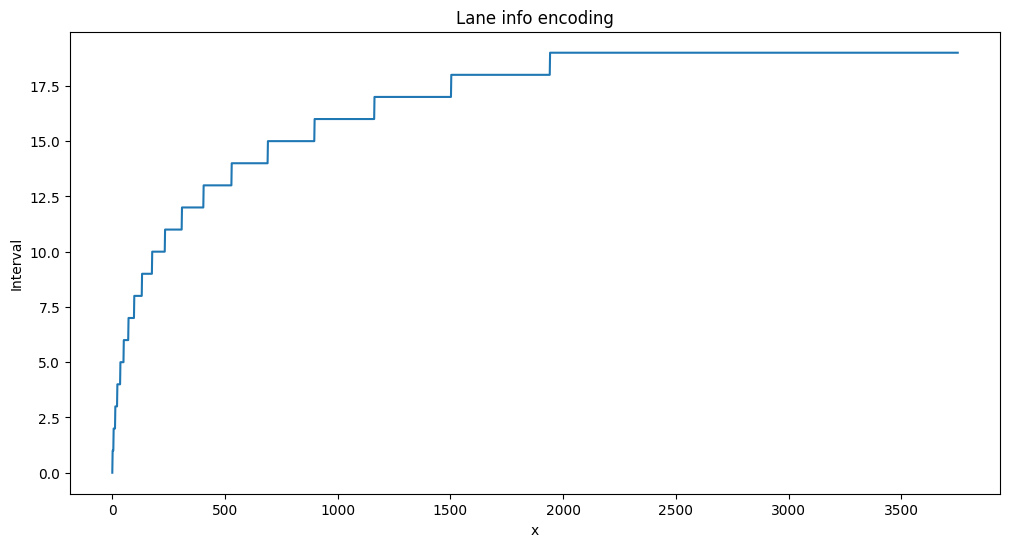
\includegraphics[width=0.78\textwidth]{imagenes/LaneInfoEncoding.png}
    \caption{Codificación por carril empleada para construir la observación local. Cada entrada de espera se transforma y conserva su correspondencia espacial con el carril de origen.}
    \label{fig:codificacion_carriles}
\end{figure}

\begin{figure}[H]
    \centering
    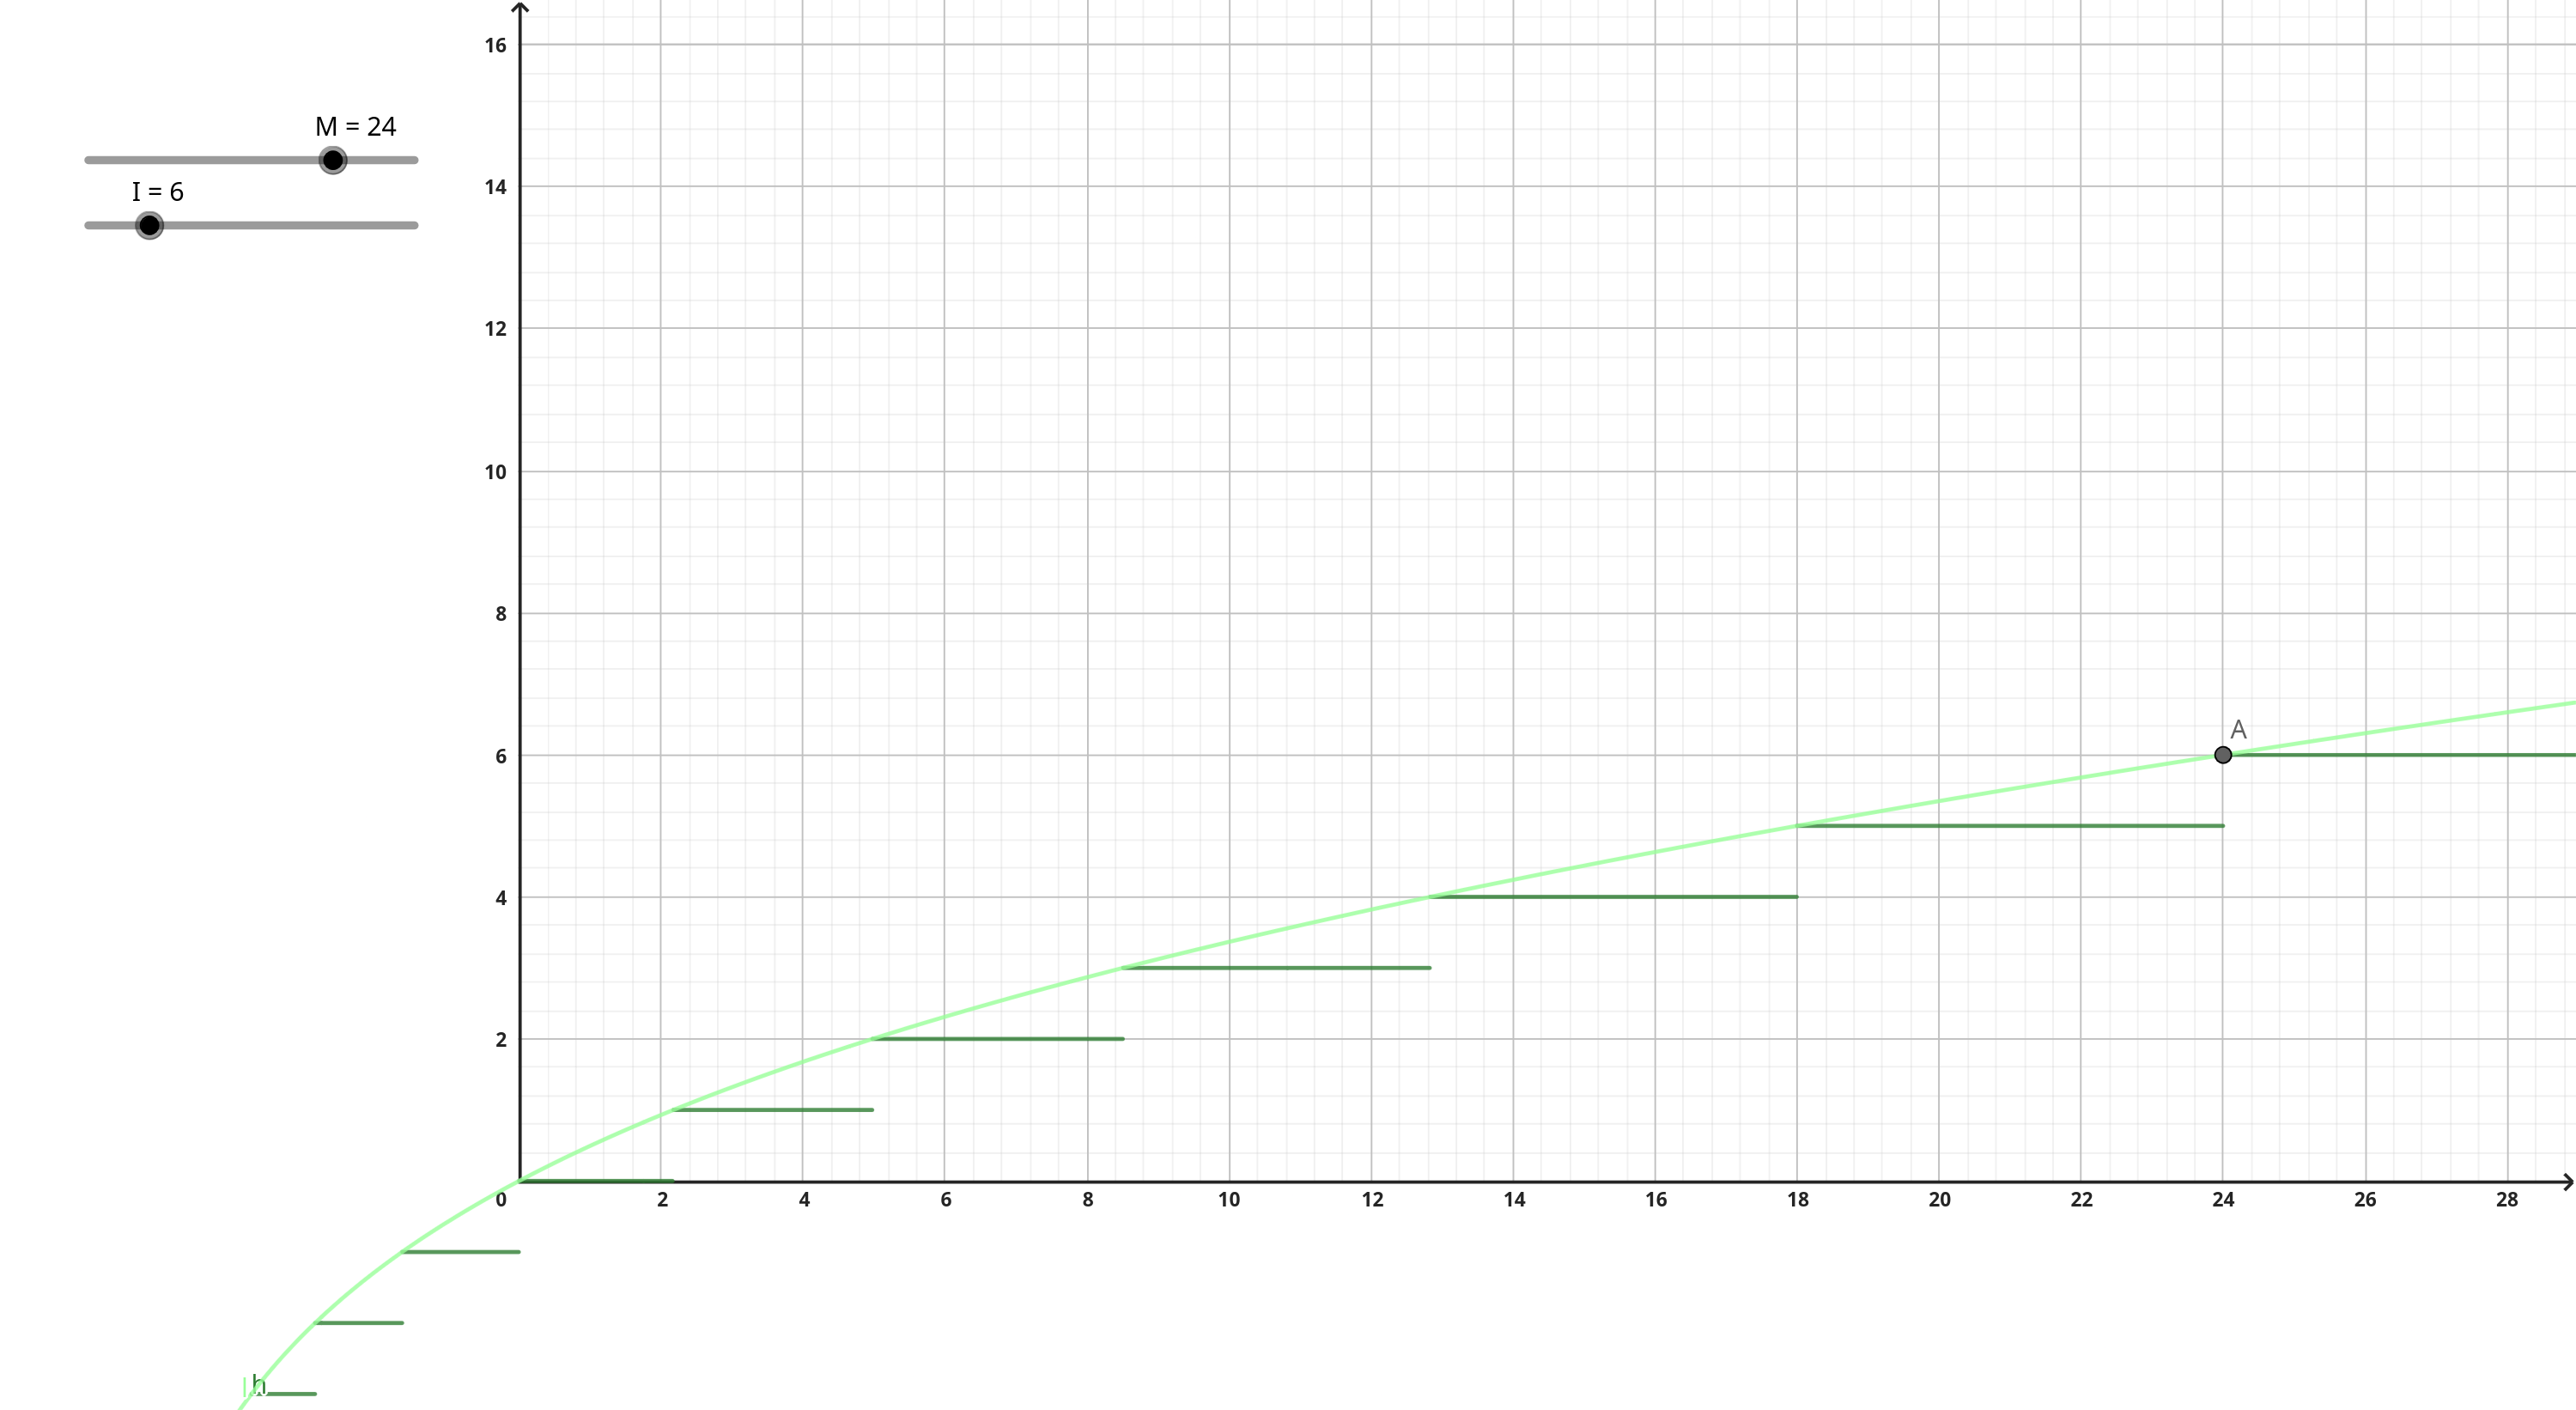
\includegraphics[width=0.78\textwidth]{imagenes/log_linear_blend_1.png}
    \caption{Ejemplo de la mezcla logarítmica-lineal utilizada por \texttt{Encoder}. La curva se interpreta como una transformación de la espera acumulada, no como una trayectoria de entrenamiento.}
    \label{fig:mezcla_log_lineal}
\end{figure}

\subsection{Espacio de Acciones y Enmascaramiento Dinámico}
\label{subsec:acciones_masking}

El espacio de acciones $\mathcal{A}_i = \{0, 1, \dots, K_i - 1\}$ representa el conjunto de fases verdes seleccionables por la intersección $i$. Los valores $m_i$ y $K_i$ difieren entre intersecciones según la geometría del cruce y las restricciones de maniobra, y cada agente dispone de un módulo de política propio sin compartición de parámetros; en ese sentido el conjunto de agentes es heterogéneo y la evaluación de \acrshort{acr-happo} se realiza sobre los espacios de observación y acción efectivos de cada escenario. En cruces con geometrías asimétricas o restricciones de maniobra, el entorno construye el conjunto de acciones admisibles y la capa personalizada \texttt{ActionMaskingTorchRLModule} aplica un enmascaramiento dinámico sobre los \glspl{logit} $z_i(a)$ antes del cómputo de la distribución \gls{softmax}. Los \glspl{logit} son puntuaciones reales sin normalizar producidas por la red; la función \gls{softmax} las transforma en probabilidades cuya suma es uno:
    \begin{equation}
\widetilde z_i(a,t) = z_i(a) + \log m_i(a,t), \qquad m_i(a,t) = \begin{cases}
    1 & \text{si } a \in \mathcal{A}^{\mathrm{adm}}_i(t) \\
    0 & \text{si } a \notin \mathcal{A}^{\mathrm{adm}}_i(t)
    \end{cases}
    \label{eq:action_mask}
    \end{equation}
donde $\mathcal{A}^{\mathrm{adm}}_i(t)\subseteq\mathcal{A}_i$ es el conjunto de acciones admisibles en el instante $t$, $m_i(a,t)$ es la máscara binaria correspondiente y $z_i(a)$ es la puntuación producida por la política. El entorno define $\mathcal{A}^{\mathrm{adm}}_i(t)=\{a_i^{\mathrm{actual}}\}$ durante una transición amarilla o mientras el tiempo de la fase corriente sea menor que $\max(t_{\min},t_{\mathrm{yellow}})$. Una vez satisfecha esa condición, quedan habilitadas las fases compatibles con la configuración del cruce. El término $\log m_i(a,t)$ vale $0$ para acciones admisibles y se limita a un entero negativo de magnitud máxima en aritmética de precisión finita para las inadmisibles, de modo que su contribución es despreciable tras la normalización. En IPPO, MAPPO y HAPPO la suma se aplica a los \textit{logits}; en IDQN se aplica a los valores $Q$ y también a la acción siguiente utilizada para el objetivo temporal, tanto en la red principal como en la red objetivo. La máscara evita acciones incompatibles, pero no reemplaza la lógica de transición amarilla del entorno, que se ejecuta después de aceptar un cambio de fase.

\subsection{Función de Recompensa Compuesta y Coordinación Vecinal}
\label{subsec:recompensa_coordinacion}

La función de recompensa representa el compromiso entre el desempeño operacional local y la cooperación distribuida. El código permite evaluar varias señales de tránsito; la selección de una señal no se interpreta como una superioridad universal, sino como una decisión experimental que se mantiene fija al comparar algoritmos dentro de un escenario. La tabla \ref{tab:alternativas_recompensa} resume las alternativas implementadas.

\begin{table}[H]
\centering
\caption{Señales de recompensa disponibles en el entorno.}
\label{tab:alternativas_recompensa}
\small
\begin{tabular}{p{4.0cm}p{7.2cm}p{3.0cm}}
\hline
\textbf{Identificador} & \textbf{Señal utilizada} & \textbf{Unidad o interpretación} \\
\hline
\texttt{diff\_halted} & Variación del número de vehículos detenidos entre pasos. & vehículos \\
\texttt{diff\_waitingTime} & Variación de la espera del último paso. & s \\
\shortstack[l]{\texttt{diff\_cumulative}\\\texttt{WaitingTime}} & Variación de la espera acumulada en los carriles de entrada. & vehículo$\cdot$s \\
\shortstack[l]{\texttt{negative\_waiting}\\\texttt{Time}\\\texttt{negative\_cumulative}\\\texttt{WaitingTime}} & Penalización directa de la espera instantánea o acumulada. & s o vehículo$\cdot$s \\
\shortstack[l]{\texttt{diff\_cumulative}\\\texttt{WaitingTime}\\\texttt{\_normalized}} & Variación acumulada dividida por la cantidad de vehículos considerada. & s \\
\texttt{pressure} & Negativo de la diferencia absoluta entre vehículos detenidos en entradas y salidas. & vehículos \\
\shortstack[l]{\texttt{negative\_queue}\\\texttt{\_length}} & Negativo de la cantidad de vehículos detenidos en los carriles de entrada. & vehículos \\
\hline
\end{tabular}
\end{table}

La tabla documenta las señales implementadas en el entorno; la disponibilidad de una clase no implica que haya sido comparada experimentalmente. En las campañas de ajuste de este capítulo se fija \texttt{reward\_key} = \path{diff_cumulative_waiting_time_with_neighbors}. Esta clave combina la señal diferencial de espera acumulada con una media sobre los vecinos mediante \texttt{NeighborhoodRelevanceReward}. En las líneas de base independientes (\acrshort{acr-ippo} e \acrshort{acr-idqn}), se fija de forma estricta $\rho_{\mathrm{coop}} = 0$, reduciendo la señal a la recompensa puramente local $R_i^{(t)} = L_i^{(t)}$. Para los métodos cooperativos (\acrshort{acr-mappo} y \acrshort{acr-happo}), el parámetro $\rho_{\mathrm{coop}} \in [0.0, 0.95]$ se optimiza mediante búsqueda bayesiana para determinar el grado óptimo de ponderación vecinal en cada escenario y arquitectura; una vez seleccionada la receta, su valor permanece fijo durante la confirmación y la evaluación reservada. No se agregan términos heurísticos adicionales. Las demás filas de la tabla se presentan como alternativas implementadas, no como funciones evaluadas, porque no existe para ellas una ejecución identificable por escenario, semilla, configuración y métrica.

\begin{enumerate}
    \item \textbf{Recompensa local diferencial ($L_i$):} cuantifica la variación del tiempo de espera acumulado entre pasos consecutivos. En esta sección, $W_{\text{acc},i}(t)$ representa la suma de los tiempos de espera de los vehículos presentes en los carriles de entrada controlados por la intersección $i$ en el paso $t$, expresada en vehículo$\cdot$segundo. La implementación activa selecciona esta señal mediante la opción de configuración \texttt{reward\_key} = \texttt{diff\_}\allowbreak\texttt{cumulative\_}\allowbreak\texttt{waiting\_}\allowbreak\texttt{time\_}\allowbreak\texttt{with\_}\allowbreak\texttt{neighbors}; su componente local utiliza esta diferencia sin dividirla por el número de vehículos. La ecuación \eqref{eq:recompensa_local} asigna una señal positiva cuando la espera disminuye:
    \begin{equation}
        L_i^{(t)} = W_{\text{acc}, i}(t-1) - W_{\text{acc}, i}(t)
        \label{eq:recompensa_local}
    \end{equation}
    \item \textbf{Señal vecinal ($N_i$):} corresponde al promedio de las señales locales obtenidas por las intersecciones del vecindario topológico directo $\mathcal{N}(i)$. Esta construcción incorpora al retorno del agente la evolución de los cruces inmediatamente conectados, pero no equivale a observar sus estados ni a optimizar una recompensa global. La ecuación \eqref{eq:recompensa_vecinal} supone $|\mathcal{N}(i)|>0$:
    \begin{equation}
        N_i^{(t)} = \frac{1}{|\mathcal{N}(i)|} \sum_{j \in \mathcal{N}(i)} L_j^{(t)}
        \label{eq:recompensa_vecinal}
    \end{equation}
    \item \textbf{Mezcla convexa:} se adopta una combinación convexa gobernada por el hiperparámetro $\rho_{\mathrm{coop}} \in [0, 0.95]$ para ponderar el componente local y el vecinal. La ecuación \eqref{eq:recompensa_compuesta} conserva las unidades de $L_i$ y $N_i$:
    \begin{equation}
        R_i^{(t)} = (1 - \rho_{\mathrm{coop}}) L_i^{(t)} + \rho_{\mathrm{coop}} N_i^{(t)} \quad \text{con} \quad \rho_{\mathrm{coop}} \in [0, 0.95]
        \label{eq:recompensa_compuesta}
    \end{equation}
    Si el vecindario es vacío, $|\mathcal{N}(i)|=0$, la implementación omite el promedio de la ecuación \eqref{eq:recompensa_vecinal} y define $R_i^{(t)}=L_i^{(t)}$. En \acrshort{acr-ippo} e \acrshort{acr-idqn}, $\rho_{\mathrm{coop}} = 0$ opera de forma fija como ancla puramente local descentralizada, garantizando que los agentes independientes no reciban retroalimentación de desempeño ajena. En \acrshort{acr-mappo} y \acrshort{acr-happo}, $\rho_{\mathrm{coop}} > 0$ modula la cooperación vecinal. En cada paso, el entorno forma el vector de recompensas $\mathbf{r}_t=(R_1^{(t)},\dots,R_N^{(t)})$ y entrega cada componente individual al módulo correspondiente; no se agregan sus componentes en una recompensa escalar global.
\end{enumerate}

\section{Implementación Algorítmica e Hiperparámetros}
\label{sec:implementacion_algoritmos}

Los cuatro algoritmos evaluados se integran en la \gls{acr-api} de Ray RLlib mediante el módulo de fábrica \texttt{algo\_factory.py}. \acrshort{acr-mappo} y \acrshort{acr-happo} utilizan \textit{learners} propios sobre PyTorch, mientras que \acrshort{acr-ippo} e \acrshort{acr-idqn} reutilizan las implementaciones de PPO y DQN de RLlib junto con módulos propios para el enmascaramiento de acciones.

\subsection{Mecanismos de Aprendizaje Independiente y Centralizado}
\label{subsec:mecanismos_algoritmos}

\begin{itemize}
    \item \textbf{\acrshort{acr-idqn} e \acrshort{acr-ippo} (Aprendizaje Independiente):} Cada intersección aprende una política local $\pi_{\theta_i}(a_i | o_i)$ tratando a los demás controladores como parte del entorno no estacionario. En \acrshort{acr-ippo}, cada agente cuenta con su propia red de valor local $V_{\phi_i}(o_i)$.
    \item \textbf{\acrshort{acr-mappo} (\acrshort{acr-ppo} Multi-Agente Centralizado \cite{yu2022surprising}):} Emplea el paradigma \acrshort{acr-ctde}. Durante la ejecución, cada actor selecciona acciones de forma descentralizada a partir de su observación local $o_i$. Durante el entrenamiento, el módulo \texttt{SharedCriticTorchRLModule} actúa como un crítico centralizado compartido multi-salida: recibe el vector de observaciones locales concatenadas $s = (o_1, o_2, \dots, o_N)$, que aporta contexto conjunto al crítico sin equivaler al estado Markoviano completo de la simulación, y produce $\mathbf{V}_{\phi}(s)=(V_{\phi,1}(s),\dots,V_{\phi,N}(s))$. Las recompensas, valores, objetivos y ventajas de \acrshort{acr-gae} ($\lambda_{\text{GAE}}$) se calculan por agente.
    \item \textbf{\acrshort{acr-happo} (\acrshort{acr-ppo} para Agentes Heterogéneos \cite{kuba2021trust}):} Su marco teórico canónico se apoya en el \textbf{Lema de Descomposición de Ventajas Multiagente}, cuya formulación utiliza una ventaja conjunta. La implementación de este trabajo constituye una adaptación: no aplica directamente ese lema, sino que inicializa los factores de actualización con ventajas individuales estandarizadas obtenidas mediante \acrshort{acr-gae} y los repondera secuencialmente. El crítico centralizado proporciona estimaciones de valor durante el entrenamiento, mientras que la reponderación secuencial descrita corresponde a la actualización de los actores; no se atribuye a esta secuencia una actualización secuencial del crítico. En cada \textit{epoch} de entrenamiento, los agentes se actualizan secuencialmente, sobre el lote completo y según un orden $(i_1, i_2, \ldots, i_N)$ re-sorteado, donde $N$ es el número total de agentes y $i_m$ es el agente ubicado en la posición $m$ de ese orden; cada actor recibe un único paso de gradiente por \textit{epoch}. Si $\overline{|A|}_i$ denota la media del valor absoluto de la ventaja individual ya estandarizada del agente $i$ en la muestra ---el conector de entrenamiento normaliza las ventajas por módulo antes de la actualización---, el hiperparámetro $p_{\text{greedy}}$ determina cómo se construye el orden: $0.0$ produce un orden aleatorio; $1.0$, un orden codicioso según $\overline{|A|}_i$; y un valor en $(0,1)$, un orden semi-codicioso que combina ambos criterios. Sea $\pi_{b}^{(i_m)}$ la política que recolectó la muestra y $\pi_{+}^{(i_m)}$ el actor de $i_m$ después de su actualización dentro del \textit{epoch} corriente. Para una observación $o$ y una acción $a$ de la muestra, la razón que se propaga a los agentes restantes es:
    \begin{equation}
        \rho_{\text{post}}^{(i_m)} = \frac{\pi_{+}^{(i_m)}(a|o)}{\pi_{b}^{(i_m)}(a|o)}
        \label{eq:happo_ratio_post_metodologia}
    \end{equation}
    La ecuación \eqref{eq:happo_ratio_post_metodologia} compara la política posterior a la actualización con la política de comportamiento que generó la muestra, el mismo denominador que utiliza el objetivo tipo \acrshort{acr-ppo} de la actualización. Para cada agente aún no actualizado $i_j$, con $j>m$, $M^{(i_j)}$ es el factor de ventaja reponderada del \textit{epoch} corriente, inicializado con su ventaja individual estandarizada al comienzo de ese \textit{epoch}. El factor se actualiza como
    \begin{equation}
        M^{(i_j)} \leftarrow M^{(i_j)} \cdot \rho_{\text{post}}^{(i_m)}, \qquad j>m.
        \label{eq:happo_factor_acumulado_metodologia}
    \end{equation}
    La ecuación \eqref{eq:happo_factor_acumulado_metodologia} incorpora al factor la razón de cada actor ya optimizado: la actualización de $i_1$ afecta a todos los agentes restantes del \textit{epoch}, la de $i_2$ a los que siguen en el orden, y así sucesivamente. Puesto que $M$ se reinicializa en cada \textit{epoch}, la propagación cubre únicamente a los agentes previos en el orden de ese \textit{epoch}, y no la secuencia completa de actualizaciones acumuladas desde la recolección.

    El procedimiento canónico de \acrshort{acr-happo} agrupa, en cambio, los pases internos de cada actor bajo un único factor secuencial; la diferencia se mantiene explícita porque afecta a la interpretación de las garantías: la mejora monótona corresponde al procedimiento teórico de región de confianza bajo sus supuestos explícitos y no se transfiere a esta variante con recorte. En la implementación evaluada, el coeficiente de la penalización de \acrshort{acr-kl} permanece fijo durante la actualización de \acrshort{acr-happo}.
\end{itemize}

La reponderación secuencial de ventajas individuales ofrece una forma de considerar políticas propias de intersecciones con acciones y condiciones de operación distintas, sin garantizar por sí misma un mejor control que MAPPO.

En los cuatro algoritmos, el entrenamiento consume observaciones del tránsito, fases ejecutadas, recompensas y observaciones siguientes para ajustar los parámetros de las redes. \acrshort{acr-idqn} conserva transiciones anteriores en un \textit{replay buffer} de episodios priorizado y multiagente; las variantes de \acrshort{acr-ppo} recolectan un \textit{rollout} con la política vigente y lo reutilizan durante una cantidad acotada de \textit{epochs}. Cada \textit{epoch} recorre el conjunto recolectado; en \acrshort{acr-ippo} y \acrshort{acr-mappo} el lote se subdivide en \textit{minibatches} y cada uno produce una actualización, mientras que en \acrshort{acr-happo} el lote no se subdivide y cada actor realiza un único paso de gradiente completo por \textit{epoch}. El optimizador, los búferes y los críticos pertenecen al proceso de aprendizaje: durante la ejecución del control, cada intersección solo necesita su observación local y la red entrenada que asigna valores o probabilidades a las fases admisibles. Por tanto, la salida del entrenamiento es una política parametrizada, no un plan semafórico fijo.

\section[Búsqueda de Hiperparámetros (HPO)]{Búsqueda de Hiperparámetros (\acrshort{acr-hpo})}
\label{sec:experimentos_hiperparametros}

La búsqueda de hiperparámetros se ejecutó con Optuna \cite{akiba2019optuna}, Ray Tune y el algoritmo de poda asíncrona \gls{acr-asha} \cite{li2020system} para las combinaciones sintéticas de algoritmo, escenario y arquitectura. La Ciudad de Mendoza se definió como un estudio separado, cuya búsqueda se inicia después del cierre de los estudios y la confirmación sintéticos. La receta sintética no se transfiere automáticamente: sus resultados pueden utilizarse, a lo sumo, para acotar el espacio de exploración de Mendoza.

Antes del muestreo se fijaron los parámetros que definen la semántica de la interacción. En particular, $\gamma=0,99$ se mantuvo constante en MAPPO, HAPPO, IPPO e IDQN como decisión de diseño informada por las configuraciones de referencia del proyecto, y no como un óptimo universal. También se fijaron la métrica de carril, la señal de recompensa y el calibrado $M_{\mathrm{lane}}$ por escenario. Las arquitecturas \texttt{h128} y \texttt{h256} no se mezclan dentro de un mismo estudio: cada una recibe un estudio independiente y se comparan después mediante métricas físicas. La métrica de carril, la recompensa, $M_{\mathrm{lane}}$ y el modo de interacción se mantienen fijos por escenario. En cambio, el número de intervalos del codificador es un hiperparámetro: modifica la resolución con que se representa cada carril y, por ello, se explora explícitamente junto con los parámetros de aprendizaje.

\begin{enumerate}
    \item \textbf{Etapa 1 (exploración bayesiana amplia):} muestreo mediante \gls{acr-tpe}. El presupuesto nominal es de 100 pruebas por combinación; el valor de 150 corresponde al límite máximo previsto para una eventual ampliación y no a una segunda etapa de búsqueda. ASHA aplica poda temprana con período de gracia de 10 iteraciones y factor de reducción 4; las pruebas podadas no integran el conjunto de candidatos finales. Se evalúan las arquitecturas compacta (\texttt{h128}: $[128, 128]$) y ancha (\texttt{h256}: $[256, 256]$) como estudios independientes de Ray Tune. El espacio registrado comprende 13 dimensiones para \acrshort{acr-mappo} y 13 parámetros nominales para \acrshort{acr-ippo}, de los cuales 12 son efectivos porque $\rho_{\mathrm{coop}}=0$ se fija. Para \acrshort{acr-happo} se registran 14 parámetros, aunque dos no modifican la actualización y el espacio efectivo comprende 12 dimensiones:
    \begin{itemize}
        \item $\rho_{\mathrm{coop}} \in [0.0, 0.95]$ (solo \acrshort{acr-mappo} y \acrshort{acr-happo}, \texttt{uniform})
        \item $\alpha_{\mathrm{lr}} \in [3\times 10^{-5}, 10^{-3}]$ (\texttt{loguniform})
        \item $\epsilon_{\mathrm{clip}} \in [0.10, 0.22]$ (\texttt{uniform})
        \item $\lambda_{\text{GAE}} \in [0.88, 0.99]$ (\texttt{uniform})
        \item $c_{\text{entropy}} \in [0.0, 0.01]$ (\texttt{uniform})
        \item $\text{grad\_clip} \in [0.25, 5.0]$ (\texttt{loguniform})
        \item $c_{\text{KL}} \in [0.05, 0.5]$ (\texttt{loguniform})
        \item $d_{\text{KL\_target}} \in [0.005, 0.03]$ (\texttt{loguniform})
        \item $\text{vf\_clip} \in [5.0, 20.0]$ (\texttt{loguniform})
        \item $K \in [5, 15]$ para \acrshort{acr-mappo} e \acrshort{acr-ippo}, y $K \in [5, 18]$ para \acrshort{acr-happo} (\texttt{randint})
        \item $N_{\text{episodes}} \in [2, 12]$ (\texttt{randint})
        \item $I \in [4, 64]$ (\texttt{randint})
        \item $B_{\text{mini}} \in \{128, 256, 512\}$ (\texttt{choice})
        \item $p_{\text{greedy}} \in [0.20, 0.90]$ (solo \acrshort{acr-happo}, \texttt{uniform})
    \end{itemize}
    Parámetros fijos: $\texttt{lane\_metric}=\texttt{acc\_waiting\_time}$, $\text{use\_kl\_loss} = \text{True}$, $\gamma=0,99$ y, para \acrshort{acr-ippo}, $\rho_{\mathrm{coop}}=0$ fijo. Para \acrshort{acr-idqn}, el espacio específico de diez dimensiones reemplaza los parámetros de \acrshort{acr-ppo} por tasa de aprendizaje $[10^{-5},10^{-3}]$, lotes $\{64,128,256,512\}$, \texttt{grad\_clip} $\in\{0,5;1;2;5;10\}$, actualización de la red objetivo $\{500,1000,2000,5000\}$ pasos, decaimiento de $\varepsilon$ en $\{5000,10000,20000\}$ pasos, $\varepsilon_{\mathrm{final}}\in[0,02,0,10]$, retorno de $n$ pasos $\{1,3,5\}$ y comienzo del aprendizaje $\{1000,2000,5000\}$ pasos, también con recompensa estrictamente local ($R_i = L_i$). En todos los algoritmos se explora $I\in[4,64]$ mediante \texttt{tune.randint(4,65)}, cuyo extremo superior no se incluye, y se fija el valor de saturación $M_{\mathrm{lane}}$ calibrado para cada escenario. En \acrshort{acr-happo}, las dimensiones asociadas al \textit{minibatch} y al objetivo de \acrshort{acr-kl} se muestrean y registran, pero no modifican su actualización, que opera con lote completo por actor y coeficiente de \acrshort{acr-kl} fijo; la búsqueda efectiva sobre \acrshort{acr-happo} comprende doce dimensiones. En los escenarios sintéticos, las semillas de entrenamiento de HPO son $\{101,137,179\}$ para $3\times1$, $3\times3$ y $4\times4\_H$, respectivamente, y las de evaluación son $\{100101,100137,100179\}$. La búsqueda en cada escenario sintético dispuso de una única semilla de entrenamiento, de modo que el ordenamiento de candidatos queda expuesto a esa realización pseudoaleatoria; la confirmación sobre diez semillas se definió para controlar ese riesgo de selección. Para Mendoza, el presupuesto y los conjuntos de semillas deben fijarse antes de iniciar su campaña y mantenerse separados de los utilizados en la evaluación reservada.
    \item \textbf{Etapa 2 (confirmación pareada):} se previó un reentrenamiento a presupuesto completo sobre las semillas de confirmación definidas por escenario. En MAPPO y HAPPO, el diseño contrasta el $\rho_{\mathrm{coop}}$ seleccionado con la línea base puramente local ($\rho_{\mathrm{coop}} = 0$). IPPO e IDQN se mantienen como líneas de base de aprendizaje independiente con recompensa puramente local, con sus propias recetas seleccionadas y las mismas reglas de evaluación reservada. Para Mendoza se definió una secuencia propia de ajuste, congelamiento y confirmación, posterior al cierre sintético. Dado que el tamaño del lote de aprendizaje forma parte del espacio de ajuste, las cuarenta iteraciones fijan el número de actualizaciones y no la experiencia total consumida; por ello, cada ejecución registra los pasos de entorno muestreados de forma acumulada (\texttt{num\_env\_steps\_sampled}) para informar, junto con el desempeño, la experiencia requerida para alcanzarlo. Las comparaciones entre familias se formulan sobre las políticas finales evaluadas bajo el mismo horizonte, la misma demanda y las mismas semillas, y no como afirmaciones de eficiencia muestral entre algoritmos.
\end{enumerate}

La selección de candidatos minimiza la métrica física \texttt{metric\_objective}, que en la campaña corresponde a la espera media estable por vehículo insertado. Sea $w_r$ la espera media de los vehículos insertados en la iteración de entrenamiento $r$. Para diagnosticar inestabilidad se calcula el incremento positivo
\begin{equation}
    X_r = \max\{0, w_r-w_{r-1}\}.
    \label{eq:incremento_espera_iteracion}
\end{equation}
La colección de realizaciones $\{X_r\}$ corresponde a \texttt{positive\_interiteration\_increases}. Para la fracción superior $\alpha_{\mathrm{CVaR}}=0,2$ se utiliza el estimador empírico de cola:
\begin{equation}
    \widehat{\operatorname{CVaR}}_{\alpha_{\mathrm{CVaR}}}(X) = \frac{1}{k}\sum_{j=1}^{k}X_{(j)}, \qquad k=\max\{1,\lceil m\alpha_{\mathrm{CVaR}}\rceil\},
    \label{eq:cvar_incrementos_espera}
\end{equation}
La ecuación \eqref{eq:cvar_incrementos_espera} reproduce el cálculo implementado: $m$ es la cantidad de incrementos finitos disponibles, $X_{(j)}$ son esos incrementos ordenados de mayor a menor y $k$ garantiza que siempre se utilice al menos una observación. Por tanto, la penalización es un promedio empírico del $20\%$ superior, no una garantía de ausencia de \textit{gridlock}. La espera $w_r$ se obtiene de \texttt{TripInfo} y se expresa en segundos por vehículo insertado.
\begin{equation}
    \text{metric\_objective}_r = w_r + 1,0 \cdot \widehat{\operatorname{CVaR}}_{0,2}(X)
    \label{eq:objetivo_estable_espera}
\end{equation}
La ecuación \eqref{eq:objetivo_estable_espera} se informa sobre las últimas 10 iteraciones, después de excluir las primeras 5 del historial de estabilidad. La primera parte prioriza una espera media baja y el segundo término penaliza aumentos recientes; el coeficiente $1,0$ es adimensional. Los candidatos se ordenan de menor a mayor por \texttt{metric\_objective}; cuando existe una métrica de evaluación válida, la espera media de evaluación se utiliza como segunda clave y, si no existe, se utiliza la espera media de entrenamiento. La ejecución debe alcanzar las 40 iteraciones y aportar métricas derivadas de \texttt{TripInfo} aptas para el ordenamiento. La completitud, la inserción, los teletransportes y la pérdida temporal se conservan para la confirmación.

\subsection{Selección y congelamiento de las configuraciones finales}
\label{subsec:seleccion_configuraciones_finales}

La selección se realiza por separado para cada combinación de algoritmo, escenario y arquitectura. Primero se consideran elegibles las pruebas que alcanzan las 40 iteraciones y aportan las métricas requeridas, derivadas de \texttt{TripInfo}: el selector exige que la métrica primaria y la secundaria estén presentes, sean convertibles a número y no sean \texttt{NaN}. La finitud de las magnitudes físicas se garantiza aguas arriba, en la extracción de métricas: el lector de \texttt{TripInfo} aborta ante atributos infinitos o negativos, valores no numéricos e identificadores de vehículo duplicados, de modo que una ejecución con telemetría inválida no produce métrica elegible.

El selector ordena a continuación por \texttt{metric\_objective} en sentido ascendente. Cuando está disponible, \texttt{tripinfo/}\allowbreak\texttt{eval\_}\allowbreak\texttt{mean\_}\allowbreak\texttt{waiting\_}\allowbreak\texttt{time\_}\allowbreak\texttt{inserted} constituye la segunda clave; en su ausencia se utiliza \texttt{tripinfo/}\allowbreak\texttt{mean\_}\allowbreak\texttt{waiting\_}\allowbreak\texttt{time\_}\allowbreak\texttt{inserted}. Esta regla mantiene un ordenamiento reproducible, aunque la segunda clave puede provenir de evaluación o de entrenamiento; esa circunstancia se registra en el manifiesto de cada receta.

Las arquitecturas \texttt{h128} y \texttt{h256} se exploran en estudios independientes y se comparan después mediante las mismas métricas físicas. La receta final conserva el identificador del estudio y del ensayo seleccionado, junto con la referencia al checkpoint generado al cierre del reentrenamiento, lo que asegura la trazabilidad de la configuración y de la política evaluada.

La receta congelada conserva todos los parámetros que determinan la interacción —\texttt{reward\_key}, \texttt{lane\_metric}, $M_{\mathrm{lane}}$ y $\gamma$— junto con los hiperparámetros de optimización seleccionados. No se modifican al evaluar las semillas reservadas del escenario correspondiente. Para Mendoza se definió una selección de recetas propia para MAPPO, HAPPO, IPPO e IDQN, sin transferencia automática desde las redes sintéticas; la limitación del aforo se trata como una restricción de validez externa y no como una razón para excluir el ajuste del controlador. La política de cada evaluación reservada proviene del reentrenamiento de la receta congelada y sus métricas no alimentan ninguna nueva decisión de ajuste.

\subsection{Infraestructura de Cómputo y Orquestación}
\label{subsec:infraestructura_hpc}

Dado el tamaño del espacio de búsqueda y el costo computacional de la simulación microscópica en \acrshort{acr-sumo}, la exploración y el entrenamiento final se desplegaron en los clústeres de cómputo \textbf{Toko} (\gls{acr-ccar} - \gls{acr-fcefn} / UNCuyo / \gls{acr-conicet}) y \textbf{Mendieta} (\gls{acr-ccad} - Universidad Nacional de Córdoba).

La ejecución distribuida se gestionó mediante el sistema de colas \acrshort{acr-slurm}. Se aplicaron las siguientes medidas:
\begin{itemize}
    \item \textbf{Aislamiento de procesos Ray en un nodo:} configuración de instancias Ray de nodo único (\texttt{setup\_ray\_single\_node}) con asignación dinámica de puertos basada en el identificador de trabajo:
    \begin{equation}
        \text{ray\_port} = 20000 + (\text{SLURM\_JOB\_ID} \pmod{20000})
        \label{eq:puerto_ray}
    \end{equation}
    La ecuación \eqref{eq:puerto_ray} transforma el identificador del trabajo en un puerto dentro de un intervalo acotado. En ella, \texttt{SLURM\_JOB\_ID} es el identificador entero del trabajo y $\pmod{20000}$ devuelve su resto al dividirlo por $20.000$. Por tanto, el puerto calculado pertenece al intervalo entero $[20000,39999]$; la fórmula reduce la probabilidad de colisión entre trabajos concurrentes, pero no constituye una reserva de puertos del sistema. Se utiliza junto con la autodetección de dirección IP mediante \texttt{hostname --ip-address}.
    \item \textbf{Gestión de E/S en almacenamiento local} (\texttt{/scratch}): para evitar saturar el sistema de archivos distribuido en red (\gls{acr-nfs}) con la telemetría microscópica de \acrshort{acr-sumo} (\texttt{tripinfo.xml}, \texttt{summary.xml}), las simulaciones y la recolección de trayectorias se ejecutaron en el almacenamiento local de cada nodo (\texttt{/scratch/\$USER/ray\_tmp/}).
    \item \textbf{Persistencia ante preempción:} los scripts de envío incorporan trampas de señales \acrshort{acr-posix} (\texttt{trap ... EXIT USR1 TERM INT}).\\
    Estas trampas sincronizan mediante \texttt{rsync} los resultados y las bases de datos SQLite de Optuna con el almacenamiento persistente del usuario (\texttt{\$HOME}), en el directorio \path{ray\_results/}. Esto permite reanudar los trabajos mediante \texttt{Tuner.restore()}.
\end{itemize}

\section{Evaluación de Rendimiento}
\label{sec:experimentos_evaluacion}

La evaluación de los modelos con hiperparámetros congelados se definió por escenario y bajo tres niveles de comparación. Cada entrenamiento independiente produce una política asociada a una semilla de entrenamiento; sus episodios de evaluación se agregan primero dentro de esa ejecución. Luego se comparan las ejecuciones independientes, que constituyen la unidad experimental.

Para los escenarios sintéticos se definieron las semillas de confirmación de entrenamiento $\{211,223,227,229,233,239,241,251,257,263\}$ y sus semillas de evaluación correspondientes $\{200211,\ldots,200263\}$. La Ciudad de Mendoza se reservó como un estudio separado, con sus propias semillas y configuración de campaña, posteriores al cierre sintético. Cada receta se evalúa sin nuevas decisiones de ajuste con las semillas reservadas del escenario. Estas semillas son diferentes de las utilizadas para seleccionar candidatos y no se las denomina \acrshort{acr-ood}, porque la demanda y la topología permanecen dentro de la familia definida para cada escenario.

Las partidas de los cuatro escenarios provienen de flujos congelados en archivos de rutas, que \acrshort{acr-sumo} convierte en vehículos durante la ejecución: en Mendoza los instantes de inserción se sortean según el proceso exponencial descrito en la sección \ref{subsubsec:mendoza_demanda_dinamica}, y en las redes sintéticas los flujos siguen intervalos regulares por \texttt{vehsPerHour}. En ambos casos la semilla de \acrshort{acr-sumo} gobierna los componentes pseudoaleatorios del simulador ---asignación de tipos vehiculares, empates de ruteo y evolución microscópica--- además de las llegadas cuando estas son estocásticas. La semilla del generador de demanda de cada escenario queda registrada en su manifiesto.

La confirmación pareada de cooperación se definió para contrastar el valor seleccionado de $\rho_{\mathrm{coop}}$ con el ancla $\rho_{\mathrm{coop}}=0$ en MAPPO y HAPPO, que son las familias para las que se implementa este contraste. IPPO e IDQN se utilizan como líneas de base de aprendizaje independiente: sus recetas se seleccionan con el mismo criterio físico de HPO y sus políticas congeladas se evalúan bajo las mismas semillas reservadas para la comparación final. A diferencia de MAPPO y HAPPO, que incorporan la recompensa cooperativa local-vecinal ($\rho_{\mathrm{coop}} > 0$) y entrenamiento centralizado, IPPO e IDQN operan exclusivamente con la señal de recompensa local ($R_i = L_i$, fijando $\rho_{\mathrm{coop}} = 0$) para representar el paradigma descentralizado e independiente.

El análisis experimental evalúa la hipótesis de si \acrshort{acr-happo} logra superar a las líneas de base de aprendizaje multiagente (\acrshort{acr-mappo}, \acrshort{acr-ippo} e \acrshort{acr-idqn}) en escenarios con disparidad de fases y heterogeneidad de flujos. De forma complementaria, cada política aprendida se contrasta contra el controlador semafórico de tiempo fijo del mismo escenario, que actúa como ancla operacional no aprendida de referencia. Para una métrica $M$ cuyo valor menor es preferible, se informa la diferencia relativa
\begin{equation}
    \Delta_M = 100\,\frac{M_{\mathrm{politica}}-M_{\mathrm{fijo}}}{M_{\mathrm{fijo}}}.
    \label{eq:diferencia_relativa_controlador}
\end{equation}
Para tasas de inserción, completitud o finalización, cuyo valor mayor es preferible, se informa además el cambio porcentual con el signo interpretado según esa dirección. La ecuación \eqref{eq:diferencia_relativa_controlador} permite comparar redes con distinta cantidad de intersecciones sin confundir una reducción absoluta de segundos con una mejora relativa.

Las métricas se presentan en tablas por escenario y algoritmo, con media, mediana, desviación estándar e intervalo de confianza del 95\% por bootstrap percentil. La unidad de remuestreo es la ejecución completa asociada a una semilla, no cada vehículo individual ni cada episodio de una misma política. Para la confirmación pareada se utiliza el procedimiento \texttt{paired\_bootstrap}: calcula la diferencia candidato menos línea base dentro de cada semilla, realiza 20.000 remuestreos con semilla $910001$ y devuelve el intervalo percentil, la diferencia media, la diferencia relativa y la proporción de remuestreos cuya media de diferencias es favorable. Esta proporción no se interpreta como una probabilidad posterior de superioridad.

El remuestreo refleja la incertidumbre de las diez ejecuciones disponibles sin aumentar el tamaño muestral: la precisión de los intervalos descansa en esa muestra. Las métricas de conteo se informan también de forma absoluta para evitar que una razón inestable o un denominador pequeño oculte el comportamiento de la red.

Cada métrica se calcula sobre una población y una ventana declaradas. La espera media de vehículos insertados utiliza como denominador los registros cuyo instante de partida pertenece a la ventana controlada; los viajes inconclusos aportan la espera observada hasta el cierre, que no equivale a su tiempo total de viaje. Si el denominador de una tasa o diferencia relativa es cero, el cambio relativo se informa como no definido y se conserva la diferencia absoluta. Para las tasas de completitud, inserción y finalización se reportan también los puntos porcentuales de diferencia. Cuando todos los tiempos de espera intersección son cero, el Gini se informa como cero por definición operacional.

La tabla \ref{tab:metricas_evaluacion} fija qué magnitudes se consideran primarias, secundarias o de control.

\begin{table}[H]
\centering
\caption{Métricas utilizadas para presentar y controlar la evaluación final.}
\label{tab:metricas_evaluacion}
\small
\begin{tabular}{p{3.8cm}p{4.4cm}p{5.4cm}}
\hline
\textbf{Métrica} & \textbf{Papel} & \textbf{Justificación} \\
\hline
Espera media de vehículos insertados & Primaria & Resume la demora experimentada por la demanda que efectivamente ingresa en la ventana controlada; es el objetivo de HPO. \\
Pérdida temporal media (\texttt{timeLoss}) & Secundaria & Captura desaceleraciones y circulación por debajo de la velocidad ideal que no siempre se reflejan en detenciones completas. \\
CR, IR y CI & Eficiencia y atención de demanda & Distinguen una política que reduce la espera de una que simplemente impide insertar vehículos o deja viajes pendientes. La CI mide específicamente la fracción de vehículos insertados en la ventana que completa su itinerario en ella. \\
Teletransportes iniciados/finalizados & Control de estabilidad & Detecta bloqueos o colapsos que SUMO resuelve mediante su mecanismo de \textit{teleport}. \\
Media, desviación, máximo, rango y Gini de espera por intersección & Equidad espacial & Indican si la mejora media se obtiene sacrificando accesos secundarios o concentrando la demora en pocos nodos. \\
\hline
\end{tabular}
\end{table}

El objetivo de HPO se utiliza exclusivamente para ordenar configuraciones; la evaluación final no reemplaza la espera media por su término de estabilidad. Se reportan por separado la espera estable, la espera media sin penalización y el incremento CVaR. No se aplican umbrales de descarte definidos después de observar los resultados: cualquier reducción de completitud, aumento de teletransportes o deterioro de equidad se muestra como resultado de control y se discute junto con la métrica primaria. Así se evita convertir una decisión posterior en un criterio de selección encubierto.

En síntesis, el diseño experimental estima el cambio de la espera media por vehículo insertado contrastando prioritariamente a HAPPO frente a MAPPO, IPPO e IDQN, utilizando el control de tiempo fijo del mismo escenario como ancla operacional de referencia, con la ejecución completa de entrenamiento como unidad experimental y con CR, IR, CI, teletransportes y equidad espacial como controles de atención a la demanda y de estabilidad. Sus principales restricciones de validez externa son el carácter restringido por datos del escenario de la Ciudad de Mendoza y la línea base de tiempo fijo generada por \acrshort{acr-sumo} ---que no reconstruye los planes semafóricos municipales---. El capítulo \ref{capitulo:resultados} presenta los resultados obtenidos con este protocolo.

\chapter{Análisis y discusión de resultados}
\label{capitulo:resultados}
En este capítulo se presentan y analizan los resultados de las ejecuciones de entrenamiento y evaluación de los algoritmos estudiados.
Con el objetivo de distinguir con claridad las etapas metodológicas del entrenamiento de los agentes, la sección se organiza en tres partes.

En primer lugar, se reportan los resultados del proceso de ajuste de hiperparámetros. En segundo lugar, se evalúan los modelos finales seleccionados en los escenarios planteados, desde redes sintéticas hasta el escenario ubicado en Ciudad de Mendoza. Finalmente, se desarrolla una discusión integradora de los hallazgos, sus implicancias y las principales limitaciones del estudio.


\section{Resultados del ajuste de hiperparámetros} 

En esta sección se resume el proceso de ajuste de hiperparámetros y se justifica la configuración utilizada en la evaluación posterior de los modelos.

\subsection{Diseño del proceso de ajuste}

\subsection{Resultados del ajuste y análisis de sensibilidad} 

\subsection{Configuración seleccionada para la evaluación final}  

\section{Resultados de los modelos finales} 

Esta sección reúne los resultados obtenidos con los modelos finales una vez fijada la configuración experimental.
La exposición se organiza según el tipo de escenario analizado. 

\subsection{Criterios de evaluación y métricas de comparación} 

\subsection{Desempeño en escenarios sintéticos: \texorpdfstring{$3\times1$, $3\times3$, $4\times4$ heterogéneo}{3x1, 3x3, 4x4 heterogéneo}}

\subsection{Desempeño en la red de carreteras de la Ciudad de Mendoza} 

Antes de evaluar los controladores, se verificó la operación del escenario canónico v14 de la Ciudad de Mendoza en los dos horizontes definidos en la sección \ref{subsubsec:mendoza_validacion_operacional}. La tabla \ref{tab:metricas_validacion_mendoza} presenta los conteos y las tasas obtenidas con el controlador de tiempo fijo; estos valores caracterizan la condición inicial del escenario y no el desempeño de las políticas aprendidas.

\begin{table}[H]
\centering
\caption{Métricas operacionales del escenario canónico v14 de la Ciudad de Mendoza bajo control de tiempo fijo.}
\label{tab:metricas_validacion_mendoza}
\setlength{\tabcolsep}{4pt}
\small
\begin{adjustbox}{max width=\textwidth}
\begin{tabular}{|l|c|c|c|c|c|c|c|}
\hline
        \textbf{Ventana temporal} & \textbf{Cargados} & \textbf{Insertados} & \textbf{Completados} & \textbf{\acrshort{acr-cr}} & \textbf{Inserción} & \textbf{Completitud} & \textit{teleport} \\ \hline
2 h ($06:30\text{--}08:30$) & 30.629 & 23.735 & 22.702 & 0,7412 & 0,7749 & 0,9565 & 0 \\ \hline
12 h ($06:00\text{--}18:00$) & 180.163 & 143.819 & 143.022 & 0,7938 & 0,7983 & 0,9945 & 0 \\ \hline
\end{tabular}
\end{adjustbox}
\end{table}

\section{Discusión e interpretación de resultados}

En esta sección se integran los resultados presentados y se discuten sus principales implicancias en relación con los objetivos del trabajo.

\chapter{Conclusiones}
\label{conclusiones}
Este capítulo sintetiza los hallazgos del estudio, relaciona la evidencia experimental con los objetivos planteados y delimita el alcance de las conclusiones. También identifica las limitaciones del modelo y propone líneas de trabajo futuro. Las afirmaciones finales deben interpretarse dentro de los escenarios, métricas y protocolos descritos en la metodología.


% APPENDIX
\appendix
\chapter{Arquitectura de Software y Patrones de Diseño}
\label{apendice:arquitectura_software}

En este apéndice se documenta la especificación arquitectónica del marco computacional \texttt{marlTLC}, su organización orientada a objetos, los diagramas de clases \acrshort{acr-uml} y los patrones de diseño previstos para desacoplar los componentes de simulación, aprendizaje por refuerzo y cálculo de recompensas. El repositorio que acompaña a este documento no contiene el código fuente completo del marco; por ello, las clases, métodos y relaciones que se presentan deben interpretarse como una especificación de diseño y no como una auditoría de archivos ejecutables.

\section{Diseño Orientado a Objetos del Entorno de Simulación}
\label{sec:apendice_uml_entorno}

El diseño del entorno separa las responsabilidades de sus componentes. En la especificación, la clase abstracta \texttt{BaseSumoEnvironment} encapsula la inicialización de \acrshort{acr-sumo}, el control temporal y la interacción de bajo nivel con la \acrshort{acr-api} \texttt{libsumo} / \texttt{traci}. A partir de ella, \texttt{SumoRllibEnv} se define como el adaptador de la simulación a la interfaz \texttt{MultiAgentEnv} de Ray RLlib.

La Figura \ref{fig:uml_entorno_agentes} ilustra el diagrama de clases \acrshort{acr-uml} correspondiente a las entidades del entorno y su relación con los controladores semafóricos. Un diagrama de clases representa los tipos de objetos que componen un programa. Cada recuadro se divide en tres partes: el nombre de la clase, sus atributos o datos almacenados y sus métodos u operaciones. El signo ``$-$'' indica un miembro de uso interno o privado; ``$+$'', uno público; y ``\#'', uno protegido, destinado a la propia clase y a sus derivadas. El texto situado después de los dos puntos indica el tipo de dato esperado. Los nombres en cursiva corresponden a clases u operaciones abstractas: definen una interfaz que debe concretarse en otra clase. Una flecha con la leyenda ``hereda de'' apunta desde la clase especializada hacia la clase general, mientras que la multiplicidad $1..*$ significa ``uno o más'' objetos relacionados.

\begin{figure}[H]
\centering
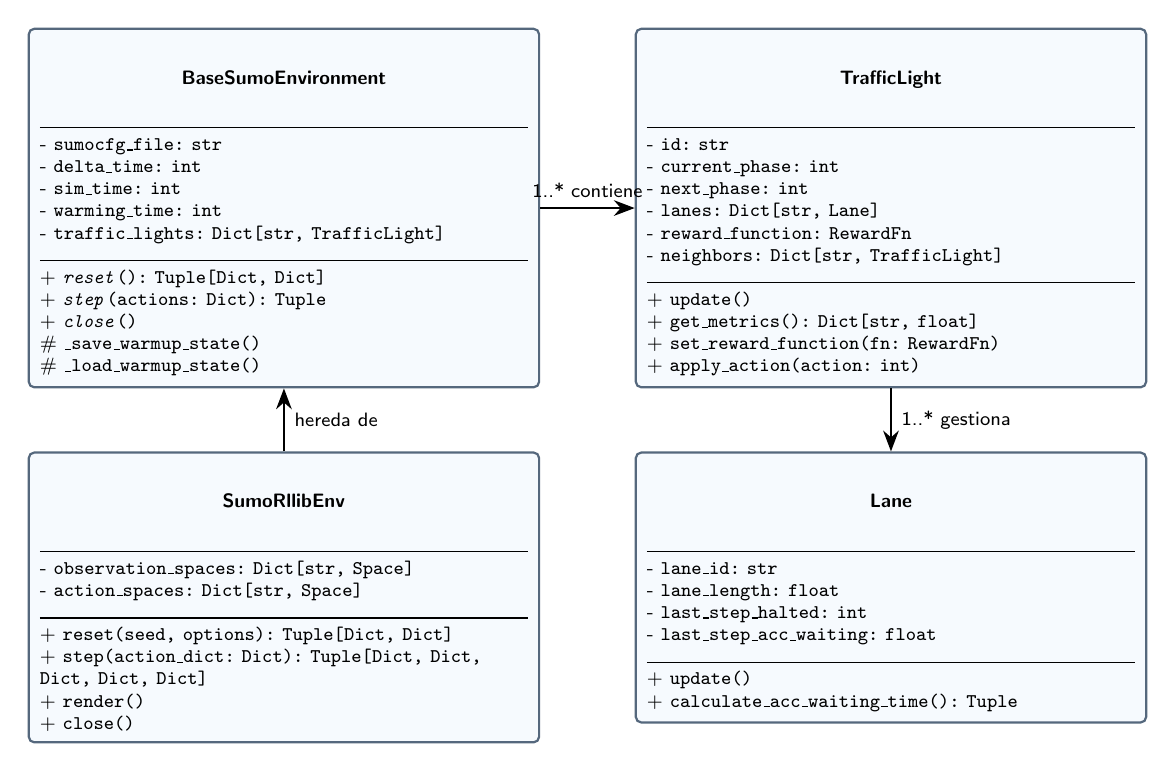
\begin{tikzpicture}[
  font=\sffamily\scriptsize,
  node distance=0.8cm and 1.2cm,
  >=Stealth,
  umlclass/.style={
    rectangle, draw=colDatoPrimario!65!black, fill=catAzulCielo!10,
    text width=6.2cm, inner sep=4pt,
    rounded corners=2pt, thick
  },
  abstractclass/.style={
    umlclass, fill=colEntorno!10
  }
]

  % BaseSumoEnvironment
  \node[abstractclass] (baseenv) {
    \begin{center}\textbf{\textit{BaseSumoEnvironment}}\end{center}
    \rule{\linewidth}{0.4pt}
    - \texttt{sumocfg\_file: str}\\
    - \texttt{delta\_time: int}\\
    - \texttt{sim\_time: int}\\
    - \texttt{warming\_time: int}\\
    - \texttt{traffic\_lights: Dict[str, TrafficLight]}\\
    \rule{\linewidth}{0.4pt}
    + \texttt{\textit{reset}(): Tuple[Dict, Dict]}\\
    + \texttt{\textit{step}(actions: Dict): Tuple}\\
    + \texttt{\textit{close}()}\\
    \# \texttt{\_save\_warmup\_state()}\\
    \# \texttt{\_load\_warmup\_state()}
  };

  % SumoRllibEnv
  \node[umlclass, below=of baseenv] (rllibenv) {
    \begin{center}\textbf{SumoRllibEnv}\end{center}
    \rule{\linewidth}{0.4pt}
    - \texttt{observation\_spaces: Dict[str, Space]}\\
    - \texttt{action\_spaces: Dict[str, Space]}\\
    \rule{\linewidth}{0.4pt}
    + \texttt{reset(seed, options): Tuple[Dict, Dict]}\\
    + \texttt{step(action\_dict: Dict): Tuple[Dict, Dict, Dict, Dict, Dict]}\\
    + \texttt{render()}\\
    + \texttt{close()}
  };

  % TrafficLight
  \node[umlclass, right=of baseenv] (tl) {
    \begin{center}\textbf{TrafficLight}\end{center}
    \rule{\linewidth}{0.4pt}
    - \texttt{id: str}\\
    - \texttt{current\_phase: int}\\
    - \texttt{next\_phase: int}\\
    - \texttt{lanes: Dict[str, Lane]}\\
    - \texttt{reward\_function: RewardFn}\\
    - \texttt{neighbors: Dict[str, TrafficLight]}\\
    \rule{\linewidth}{0.4pt}
    + \texttt{update()}\\
    + \texttt{get\_metrics(): Dict[str, float]}\\
    + \texttt{set\_reward\_function(fn: RewardFn)}\\
    + \texttt{apply\_action(action: int)}
  };

  % Lane
  \node[umlclass, below=of tl] (lane) {
    \begin{center}\textbf{Lane}\end{center}
    \rule{\linewidth}{0.4pt}
    - \texttt{lane\_id: str}\\
    - \texttt{lane\_length: float}\\
    - \texttt{last\_step\_halted: int}\\
    - \texttt{last\_step\_acc\_waiting: float}\\
    \rule{\linewidth}{0.4pt}
    + \texttt{update()}\\
    + \texttt{calculate\_acc\_waiting\_time(): Tuple}
  };

  % Relaciones
  \draw[->, thick, line width=1pt] (rllibenv) -- node[right] {hereda de} (baseenv);
  \draw[->, thick, line width=1pt] (baseenv) -- node[above] {1..* contiene} (tl);
  \draw[->, thick, line width=1pt] (tl) -- node[right] {1..* gestiona} (lane);

\end{tikzpicture}
\caption[Diagrama de clases del entorno de simulación y de sus relaciones principales.]{Diagrama de clases \acrshort{acr-uml} del entorno. \texttt{SumoRllibEnv} hereda la interfaz de \texttt{BaseSumoEnvironment}; el entorno contiene uno o más objetos \texttt{TrafficLight}, y cada controlador semafórico gestiona uno o más objetos \texttt{Lane}. En cada clase se muestran sus principales atributos y métodos.}
\label{fig:uml_entorno_agentes}
\end{figure}

La Figura \ref{fig:uml_entorno_agentes} se organiza desde la abstracción general hacia las entidades de la red. En la columna izquierda, \texttt{BaseSumoEnvironment} concentra el archivo de configuración, los parámetros temporales, los controladores y las operaciones generales de reinicio, avance y cierre. Debajo, \texttt{SumoRllibEnv} especializa esa clase para recibir un diccionario de acciones de los agentes y devolver las observaciones, recompensas y estados definidos por la interfaz de Ray RLlib. A la derecha, el diseño asigna a \texttt{TrafficLight} la fase actual, la siguiente fase, sus carriles, su función de recompensa y sus vecinos; también le asigna la actualización de métricas y la aplicación de acciones. Finalmente, \texttt{Lane} representa la longitud y las medidas recientes de detención y espera. Las flechas muestran las dependencias previstas entre la interfaz de aprendizaje, el entorno, los controladores y sus carriles.

\section{Jerarquía de Funciones de Recompensa y Patrón Strategy}
\label{sec:apendice_uml_recompensas}

En la especificación, el cálculo de la recompensa se desacopla mediante el patrón \textbf{Strategy}. Esta organización permite sustituir la métrica de optimización sin modificar el bucle principal de simulación.

La clase base abstracta \texttt{RewardFn} define la interfaz común \texttt{compute\_reward(tl\_id)}. En el diseño se contemplan formulaciones locales basadas en tres señales: demora acumulada, longitud de cola y presión de red. La coordinación distribuida se representa mediante el patrón \textbf{Composite}: una clase de recompensa compuesta combina la señal local y la señal promedio de los semáforos adyacentes.

La Figura \ref{fig:uml_recompensas} detalla las clases que intervienen directamente en la recompensa cooperativa. Las demás estrategias locales registradas en el sistema no se dibujan para conservar la legibilidad. Se mantienen las convenciones explicadas para la Figura \ref{fig:uml_entorno_agentes}; en este segundo diagrama, la flecha discontinua rotulada ``compone'' indica que una clase utiliza otra como parte de su cálculo, no que herede sus atributos y métodos.

\begin{figure}[H]
\centering
\resizebox{0.98\textwidth}{!}{%
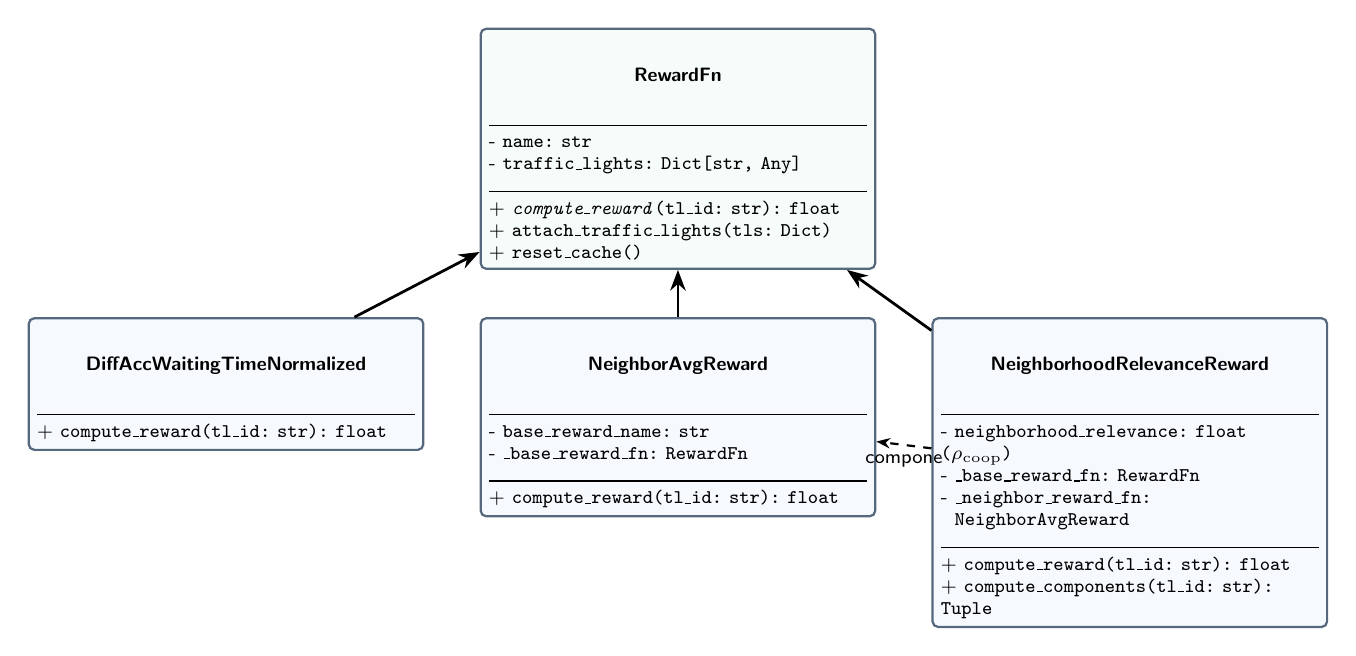
\begin{tikzpicture}[
  font=\sffamily\scriptsize,
  node distance=0.6cm and 0.5cm,
  >=Stealth,
  umlclass/.style={
    rectangle, draw=colDatoPrimario!65!black, fill=catAzulCielo!10,
    text width=4.8cm, inner sep=3pt,
    rounded corners=2pt, thick
  },
  abstractclass/.style={
    umlclass, fill=colInterfaz!10
  }
]

  % RewardFn (Abstract)
  \node[abstractclass] (rewardfn) {
    \begin{center}\textbf{\textit{RewardFn}}\end{center}
    \rule{\linewidth}{0.4pt}
    - \texttt{name: str}\\
    - \texttt{traffic\_lights: Dict[str, Any]}\\
    \rule{\linewidth}{0.4pt}
    + \texttt{\textit{compute\_reward}(tl\_id: str): float}\\
    + \texttt{attach\_traffic\_lights(tls: Dict)}\\
    + \texttt{reset\_cache()}
  };

  % DiffAccumulatedWaitingTimeReward
  \node[umlclass, below left=of rewardfn, xshift=-0.2cm] (diffacc) {
    \begin{center}\textbf{DiffAccWaitingTimeNormalized}\end{center}
    \rule{\linewidth}{0.4pt}
    + \texttt{compute\_reward(tl\_id: str): float}
  };

  % NeighborAvgReward
  \node[umlclass, below=of rewardfn] (neighavg) {
    \begin{center}\textbf{NeighborAvgReward}\end{center}
    \rule{\linewidth}{0.4pt}
    - \texttt{base\_reward\_name: str}\\
    - \texttt{\_base\_reward\_fn: RewardFn}\\
    \rule{\linewidth}{0.4pt}
    + \texttt{compute\_reward(tl\_id: str): float}
  };

  % NeighborhoodRelevanceReward
  \node[umlclass, below right=of rewardfn, xshift=0.2cm] (neighrel) {
    \begin{center}\textbf{NeighborhoodRelevanceReward}\end{center}
    \rule{\linewidth}{0.4pt}
    - \texttt{neighborhood\_relevance: float ($\rho_{\mathrm{coop}}$)}\\
    - \texttt{\_base\_reward\_fn: RewardFn}\\
    - \texttt{\_neighbor\_reward\_fn:}\\
    \phantom{- }\texttt{NeighborAvgReward}\\
    \rule{\linewidth}{0.4pt}
    + \texttt{compute\_reward(tl\_id: str): float}\\
    + \texttt{compute\_components(tl\_id: str): Tuple}
  };

  % Relaciones
  \draw[->, thick, line width=1pt] (diffacc) -- (rewardfn);
  \draw[->, thick, line width=1pt] (neighavg) -- (rewardfn);
  \draw[->, thick, line width=1pt] (neighrel) -- (rewardfn);
  \draw[-{Stealth[length=5pt]}, dashed, thick, line width=0.8pt] (neighrel) -- node[below, font=\sffamily\scriptsize] {compone} (neighavg);

\end{tikzpicture}%
}
\caption[Especificación UML del módulo de recompensas.]{Especificación \acrshort{acr-uml} del módulo de recompensas. Las clases inferiores se definen como realizaciones de \texttt{RewardFn}; la clase compuesta incorpora la señal promedio de los controladores vecinos.}
\label{fig:uml_recompensas}
\end{figure}

La Figura \ref{fig:uml_recompensas} sitúa a \texttt{RewardFn} en la parte superior porque define la operación común \texttt{compute\_reward}, que recibe el identificador de un controlador semafórico y devuelve un valor numérico. Las tres flechas ascendentes indican que las clases inferiores se especializan para proporcionar variantes de esa operación. \texttt{DiffAccWaitingTimeNormalized} representa una señal local normalizada a partir de la variación del tiempo de espera acumulado, mientras que \texttt{NeighborAvgReward} promedia la señal base de los controladores vecinos. \texttt{NeighborhoodRelevanceReward} conserva ambas funciones y las combina según $\rho_{\mathrm{coop}}$, el peso de cooperación vecinal. La flecha discontinua entre las dos últimas clases muestra esa relación de composición. Esta separación permite cambiar la formulación de la recompensa sin modificar el bucle que avanza la simulación.

\section{Patrones de Diseño Implementados}
\label{sec:apendice_patrones_diseno}

A continuación se resumen los patrones contemplados en la especificación de \texttt{marlTLC}. La lista describe responsabilidades y relaciones de diseño; no certifica la presencia de una implementación ejecutable de cada componente en el repositorio.

\begin{enumerate}
    \item \textbf{Patrón Strategy (Estrategia):}
    \begin{itemize}
        \item \textbf{Propósito:} encapsular los algoritmos de recompensa para intercambiarlos sin modificar los controladores semafóricos.
        \item \textbf{Rol en el diseño:} interfaz base \texttt{RewardFn} y variantes concretas de recompensa.
    \end{itemize}

    \item \textbf{Patrón Factory Method y Registry (Fábrica con Registro Dinámico):}
    \begin{itemize}
        \item \textbf{Propósito:} instanciar funciones de recompensa y módulos neuronales a partir de cadenas de configuración o especificaciones compuestas (\texttt{RewardSpec}). También permite registrar nuevas funciones sin modificar la fábrica, de acuerdo con el principio abierto/cerrado.
        \item \textbf{Rol en el diseño:} registro mediante \texttt{RewardFactory} y \texttt{@register\_reward}, que identifica el mecanismo previsto para asociar nombres de configuración con funciones de recompensa.
    \end{itemize}

    \item \textbf{Patrón Composite (Objeto Compuesto):}
    \begin{itemize}
        \item \textbf{Propósito:} combinar recompensas locales y vecinales mediante una interfaz uniforme.
        \item \textbf{Rol en el diseño:} clases de recompensa compuesta que agregan señales locales y vecinales.
    \end{itemize}

    \item \textbf{Patrón Protocol / Structural Subtyping (Tipado Estructural):}
    \begin{itemize}
        \item \textbf{Propósito:} desacoplar el proveedor de métricas vecinales del tipo concreto \texttt{TrafficLight}, facilitando las pruebas unitarias con objetos simulados (\textit{mocks}) y evitando dependencias circulares.
        \item \textbf{Rol en el diseño:} protocolo \texttt{NeighborInfoProvider} para describir la información vecinal requerida sin depender de una clase concreta. El detalle del decorador de comprobación en tiempo de ejecución no forma parte de la evidencia disponible en este repositorio.
    \end{itemize}

    \item \textbf{Patrón Adapter (Adaptador):}
    \begin{itemize}
        \item \textbf{Propósito:} traducir la \acrshort{acr-api} procedural y basada en comandos de \acrshort{acr-traci} / \texttt{libsumo} a la interfaz orientada a objetos de \texttt{MultiAgentEnv} (Ray RLlib).
        \item \textbf{Rol en el diseño:} \texttt{SumoRllibEnv} como punto de adaptación entre el simulador y la interfaz de aprendizaje.
    \end{itemize}

    \item \textbf{Patrón Decorator (Decorador):}
    \begin{itemize}
        \item \textbf{Propósito:} extender dinámicamente las capacidades de los módulos sin alterar su jerarquía de herencia.
        \item \textbf{Rol en el diseño:} decoradores de registro y una envoltura para los módulos de acción en PyTorch; los nombres concretos de esas piezas se mantienen como identificadores de la especificación.
    \end{itemize}
\end{enumerate}


% REFERENCES
\bibliographystyle{babalpha}
\bibliography{bibliografia}

\end{document}
